\begin{savequote}[10cm]

  ``I kind of lost track of time...''\newline
  ``For two hours?''\newline
  Elend nodded sheepishly. ``There were books involved.''
  
  \qauthor{--― Brandon Sanderson, \textit{The Well of Ascension}}
\end{savequote}

\chapter{Ancient Admixture into Africa from the Ancestors of non-Africans} \label{ch:aaa}

%Text and figures in this chapter have been largely adopted from:

%{\small \fullcite{Cole2020} }

%and 

%{\small \fullcite{10.1371/journal.pone.0247647}}



% \begin{quote}
%     \noindent \small Genetic diversity across human populations has been shaped by demographic history, making it possible to infer past demographic events from extant genomes. 
%     Next generation sequencing of diverse populations has allowed for the possibility of understanding foundational events in human evolution, however methodological barriers lie between these complex datasets and meaningful inference. 
%     In this chapter, I apply the extensions made to the SMCSMC framework to infer directional migration alongside population size in a poorly understood period of history, the Late Middle Paleolithic and the Out of Africa migration. 
%     I find evidence for substantial migration from the ancestors of present-day Eurasians into African groups between 40 and 70 thousand years ago, predating the divergence of Eastern and Western Eurasian lineages. In addition, I present suggestive evidence that this lineage diverged from the remainder of the migrants before their interbreeding event with Neanderthals. This migration event accounts for previously unexplained genetic diversity in African populations around this epoch, and supports the existence of novel population substructure in the Late Middle Paleolithic. Additionally, I demonstrate the importance of parameterizing the full migration matrix for the inference of other demographic parameters of interest. These results indicate that our species' demographic history around the out-of-Africa event is more complex than previously appreciated. 
% \end{quote}


\minitoc

% Sequencing data from diverse populations is allowing for equity surrounding the understanding of genetic disease, but has also opened the door for a nuanced exploration of the historical relationship between populations worldwide, allowing previously unknown interactions to be elucidated. 
% Why machine learning?
%   Traditionally, summary statistics have been used to aggregate over information provided by polymorphisms. The famous F_st measure being one of the most widely known, and more modern adaptations such as drift statistics provide a formal framework for quantifying shared genetic drift given the assumption of no selection. 
%   However, these methods are not able to capture the variation encoded in one of the fields most enigmatic data structures, the ancestral recombination graph. the search space here is too large for any analytical inference, even when using diffusion based appraoches. 
%   The main motivation for using machine learning, here more specifically stochastic inference, is to learn simultaneously realistic recombination breakpoints (the points at which a geneological tree in the genome transforms into another) and the individual trees. This is a task which must be approached through stochastic inference, as inferring these data structures 


\section{Introduction}

The history of a population shapes its patterns of genetic diversity. A nuanced understanding of the historical relationships between global populations has been hindered by both the lack of availability genomic sequencing data and methodological barriers. With the recent completion of several repositories of genomic variation across the globe, and the advances presented in the previous chapter allowing for tractable inference of directional migration rates, here I aim to investigate ancient contributors to extant genomic variation using machine learning and sequence data. 

Before the era of \gls{ngs}, an understanding of diverse populations was mostly based on combinations of variants in Y chromosome and \gls{mtDNA}. Genotype frequency data from microarrays has been used more recently, and will be discussed in the following section. As the Y chromosome and mtDNA do not recombine, each comprise a single genealogical tree dating back to a common ancestor. This attractive analytical property allowed geneticists in the late twentieth century to study the evolution of these two lineages in great depth, leading to an extensive catalog of variation within so-called haplogroups (see \url{https://isogg.org/tree/index.html}). As \gls{mtDNA} is inherited maternally and Y chromosome DNA is inherited paternally, they represent unique viewpoints into sexually dimorphic anthropological processes (for a review, see \textcite{Kivisild2015}). Results from haplogroup analyses have motivated many important discoveries, however caution must be taken when interpreting the results of a single tree in light of the whole of human history \cite{Rubinoff2005}. While these single trees are constrained by the overall demographic process, they are not representative of it due to incomplete lineage sorting. With recent access to high quality \gls{wgs} data, we are able to efficiently sample many more of the marginal trees along the genome. Therefore, for the general case of investigating population structure across the globe in light of human history, the nuclear genome must be focus of our study.

Before the advent of \gls{ngs}, patterns in genomic diversity have been investigated through differences in allele frequencies between subpopulations. 
Metrics such as the fixation index are often used to summarize differences between subsets of the population, either in terms of their relative variances, their probability of \gls{ibd} or their \gls{tmrca} \cite{Holsinger2009}. 
Modern adaptations and extensions of Wright's F statistics include so-called drift statistics, which quantity the degree to which two populations share genetic drift \cite{Patterson2012}. These statistics can be built up to create intricate descriptions and statistical tests for shared drift, ($f_3$) admixture ($D$, $f_4$), number of introgression events ({\tt qpWave}) and even entire global topologies of population differentiation with branch lengths ({\tt qpAdm}) \cite{Petr2019}. These approaches form a highly useful toolkit for studying easy to gather polymorphism data, but do not attempt to recapitulate the processes by which this variation is produced. Critically, they do not attempt to reconstruct demographic parameters over time. In order to explore this much larger parameter space, machine learning is necessary. 

How a given set of individuals are related at a particular locus is represented by a phylogenetic tree.  Because of past recombination events, this tree changes along the genome, resulting in a series of trees that may be represented in a data structure known as the ancestral recombination graph. \cite{Rasmussen2014}. 
All information about the genealogical history of a set of individuals can be encoded in their ARG, and having access to the ARG would help immensely when making statements of a population’s demographic history.  However, the ARG cannot be observed directly \cite{Speidel2019}. 
Recently, methods which use stochastic inference techniques have been able to directly sample from the posterior distribution of marginal genomic trees and produce representations of probable ancestral recombination graphs \cite{Speidel2019, Kelleher2019, Rasmussen2014}.

%Methods for doing this inference analytically are currently outside the scope of the field, so machine learning based approaches which learn probable representations from data represent a crucial element of \gls{arg} inference. 
Currently, no analytical methods for inferring ARGs are known, and it seems likely that none exist.  
Therefore, several researchers have developed approximate statistical inference techniques, such as ArgWeaver-D, tsInfer, Relate, and \gls{smc2} \cite{Speidel2019,Kelleher2019,Rasmussen2014,10.1371/journal.pone.0247647}.
I extend the approach taken by \gls{smc2} to infer directional migration rates simultaneously with effective population size, enabling a unique viewpoint into the ancient past.


%Methods to characterize demographic history from genetic data alone form a useful and independent complement to archaeological approaches \cite{Nielsen2017a}, and many methods have been developed for this purpose \cite{Li2011,Pickrell2012,Rasmussen2014,Schiffels2014,Mathieson2014,Steinrucken2015,Malaspinas2016,Chikhi2018,Speidel2019,Kelleher2019,Wang2019a,Albers2019}. 
A particularly interesting time in human history is the end of the Middle Paleolithic approximately $\sim$60 ka BP, which saw the divergence of the most deeply sampled lineages of human genetic variation, introgression from multiple archaic sources, and the expansion of anatomically modern humans Out of Africa. 
As archaeological evidence and ancient DNA from this period are scarce, inference of demography from present-day genetic data is potentially very informative, though technically challenging. Here, we use the previously developed approach, SMCSMC, to infer population size and directional migration in a unique and dynamic period of ancient human development.

This chapter is structured as follows. Firstly, I give an introduction to pertinent historical and anthropological theories relating to this period of time to orient the reader. Secondly, I introduce competing approaches for the inference of ancestral recombination graphs and motivate the usage of SMCSMC for this application. Following this, I outline my contributions to this area of research, which involve the identification and characterization of a putative directional migration from the ancestors of modern day Eurasians to the ancestors of modern day Africans. 


\subsection{Out of Africa and the peopling of Eurasia}

An abundance of archaeological and genetic evidence has shown that the continent of Africa is the historical source of all modern humans \cite{Lopez2015}. It contains more genetic sequence diversity than any other region of the world, so much so that on average, the two haplotypes that comprise a single African genome are less similar than two haplotypes taken anywhere outside the continent. \cite{Mallick2016}. Evidence from climate science suggests that a combination of a gradual shift away from aridity in Northern Africa as well as short term dry-wet cycles may have motivated both global and local range expansions \cite{Schaebitz2021, Timmermann2016}. The most pertinent of these range expansions is the migration Out of Africa and into Eurasia, an event which has formed the basis of modern population structure around the globe. 
The individual migrants involved in this event probably diverged from sister populations within the continent for many tens of thousands of years before their eventual dispersal into the Levant and beyond \cite{Bergstrom2019, Schiffels2014}. The population which formed this successful range expansion out of Africa experienced at least one, and potentially multiple, breeding events with Neanderthals \cite{Sankararaman2012}. Eventually, the group split into two distinct subpopulations around the time of the Ust'-Ishim individual, approximately 45 ka BP \cite{Fu2014}. One of these populations went East, forming the basis of for East Asians and Aboriginal Australians, while the other went West, forming the initial Upper Paleolithic European hunter-gatherers \cite{Skoglund2017,Lipson2017}. These were not the only derivative groups from the original Out of Africa, as another earlier diverged population popularly known as ``Basal Eurasians'' are thought to have branched before the initial contact with Neanderthal populations and contribute to later European population structure \cite{Lazaridis2014}. From this point on, diversification occurred on a highly regional basis, beyond the scope of this brief review. 

% Extinct populations
% Former evidence of back migration
Little is known about population structure within Africa prior to the expansion of agriculturalists and pastoral groups \cite{Busby2016, Patin2017}. Recent evidence from the handful of successfully sequenced ancient African genomes hint at large-scale population movements and admixture from multiple highly divergent, extinct populations, with complex affinities to current groups \cite{Skoglund2018, Lipson2019, GallegoLlorente2015a}. The majority of structure in the continent is derived from events in the Holocene, including the spread of Bantu languages from Western Central Africa both East and South, as well as admixture from pastoralists in the Near East and Western Eurasia \cite{Busby2016}. Eastern Africans are the most closely related group to the ancestral Out of Africa migrants, though they show particularly high levels of ancestry related to neolithic populations from Iran and the Levant consistent with multiple waves of back-migration in the Holocene \cite{Skoglund2017}.  
Evidence for recent admixture from Eurasian sources is well established, however the lack of ancient African DNA from the Pleistocene has confounded efforts to uncover interactions between the earliest inhabitants of the continent.
While the migration event associated with establishing current global population structure has been confidently dated between 60-80 ka BP, \gls{cahg} and \gls{sahg} such as the Mbuti and KhoeSan (without implying linguistic unity, defined as southern African hunter-gatherers who speak non-Bantu languages which include a click consonant) may have diverged from other groups 200-250 ka BP \cite{Lipson2019, Schlebusch2017}. 
In the intervening millennia, fossils identified as AMH have been found in China about 80-120kya, Sumatra about 63-73 ka BP, and artifacts from Australia 65 ka BP \cite{Clarkson2017, Liu2015, Westaway2017}.
Support for multiple migrations across Eurasia additionally comes from climate science, where four distinct periods of warming may have provided vegetated migration routes out of Africa (OoA) as early as 120 ka BP \cite{Timmermann2016}.
The extent of contributions to modern day populations from ``ghost'' populations is unknown, though controversially suggested in Australasia and South East Asia \cite{Malaspinas2016, Mallick2016, Pagani2016, Rasmussen2011, Skoglund2015} and Africa  \cite{Durvasula2019, Speidel2019, Lipson2019, Hammer2011, Plagnol2006, Ragsdale2019}.
To a large degree, the fate of these anciently diverged populations and their contributions, if any, to modern day populations remains an open question. 
Using an extension to \gls{smc2}, I aim to use machine learning to investigate ancient contributions to modern day population structure within global \gls{ngs} datasets.



\section{Methods}

\subsection{A Particle Filter for Demographic Inference} Details of the Sequential Monte Carlo for the Sequentially Markovian Coalescent (SMCSMC) algorithm have been previously published \cite{Henderson2018} (see the URLs for an implementation). 
Briefly, SMCSMC builds an approximation of the posterior distribution of genealogical trees conditional on observed mutations along the genome using a particle filter, a method also known as sequential Monte Carlo sampling. It does so by simulating a number of sequences of genealogical trees (particles) under a fixed set of demographic parameters $\theta$ using the sequential coalescent sampler {\tt SCRM} \cite{Staab2015}. Simulated recombination events may change the local trees along the sequence. Particles are then weighted according to their conditional likelihood given observed polymorphisms.  To avoid sample depletion, the set of particles is regularly resampled, which tends to remove and duplicate particles with low and high weight respectively.  To further increase the efficiency of the procedure, the resampling procedure targets not the partial posterior distribution that includes polymorphisms up to the current location, but also includes a "look-ahead likelihood" term that approximates a particle's likelihood's dependence on subsequent polymorphisms, while ensuring that the estimate of the posterior tree distribution remains asymptotically exact.  From a sample of trees from the posterior distribution, Variational Bayes (VB) or Stochastic Expectation Maximization (SEM) is used to update the estimates of demographic parameters $\hat{\theta}$. This is repeated over a given number of iterations, or until the estimate of $\theta$ has converged.

To add the ability to infer time-varying migration rates, we exploit the capabilities of SCRM to simulate ARGs under complex demographic scenarios, and collect sufficient statistics (migration opportunity, and number, time and direction of simulated migration events) for each particle. 

We use SMCSMC to infer effective population sizes and migration matrices in pairs of unrelated individuals from the phased release of the Simons Global Diversity Panel. We set a uniform recombination rate of $3\times10^{-9}$ and a neutral mutation rate of $1.25\times10^{-8}$, both in units of events per nucleotide per generation; previous results indicate that modeling recombination
hotspots minimally affects results \cite{Li2011}. To reduce the number of iterations to convergence, we initialise the particle filter with an approximation of human demographic history (\Cref{fig:smc2demog}).
We seed the model with an initial constant symmetric  migration rate of 0.0092 ($M_{i,j}$; proportion per generation of the sink population replaced by migrants from the source backwards in time). We arrive at this value through simulation (data not shown).

\begin{figure}
	\centering
	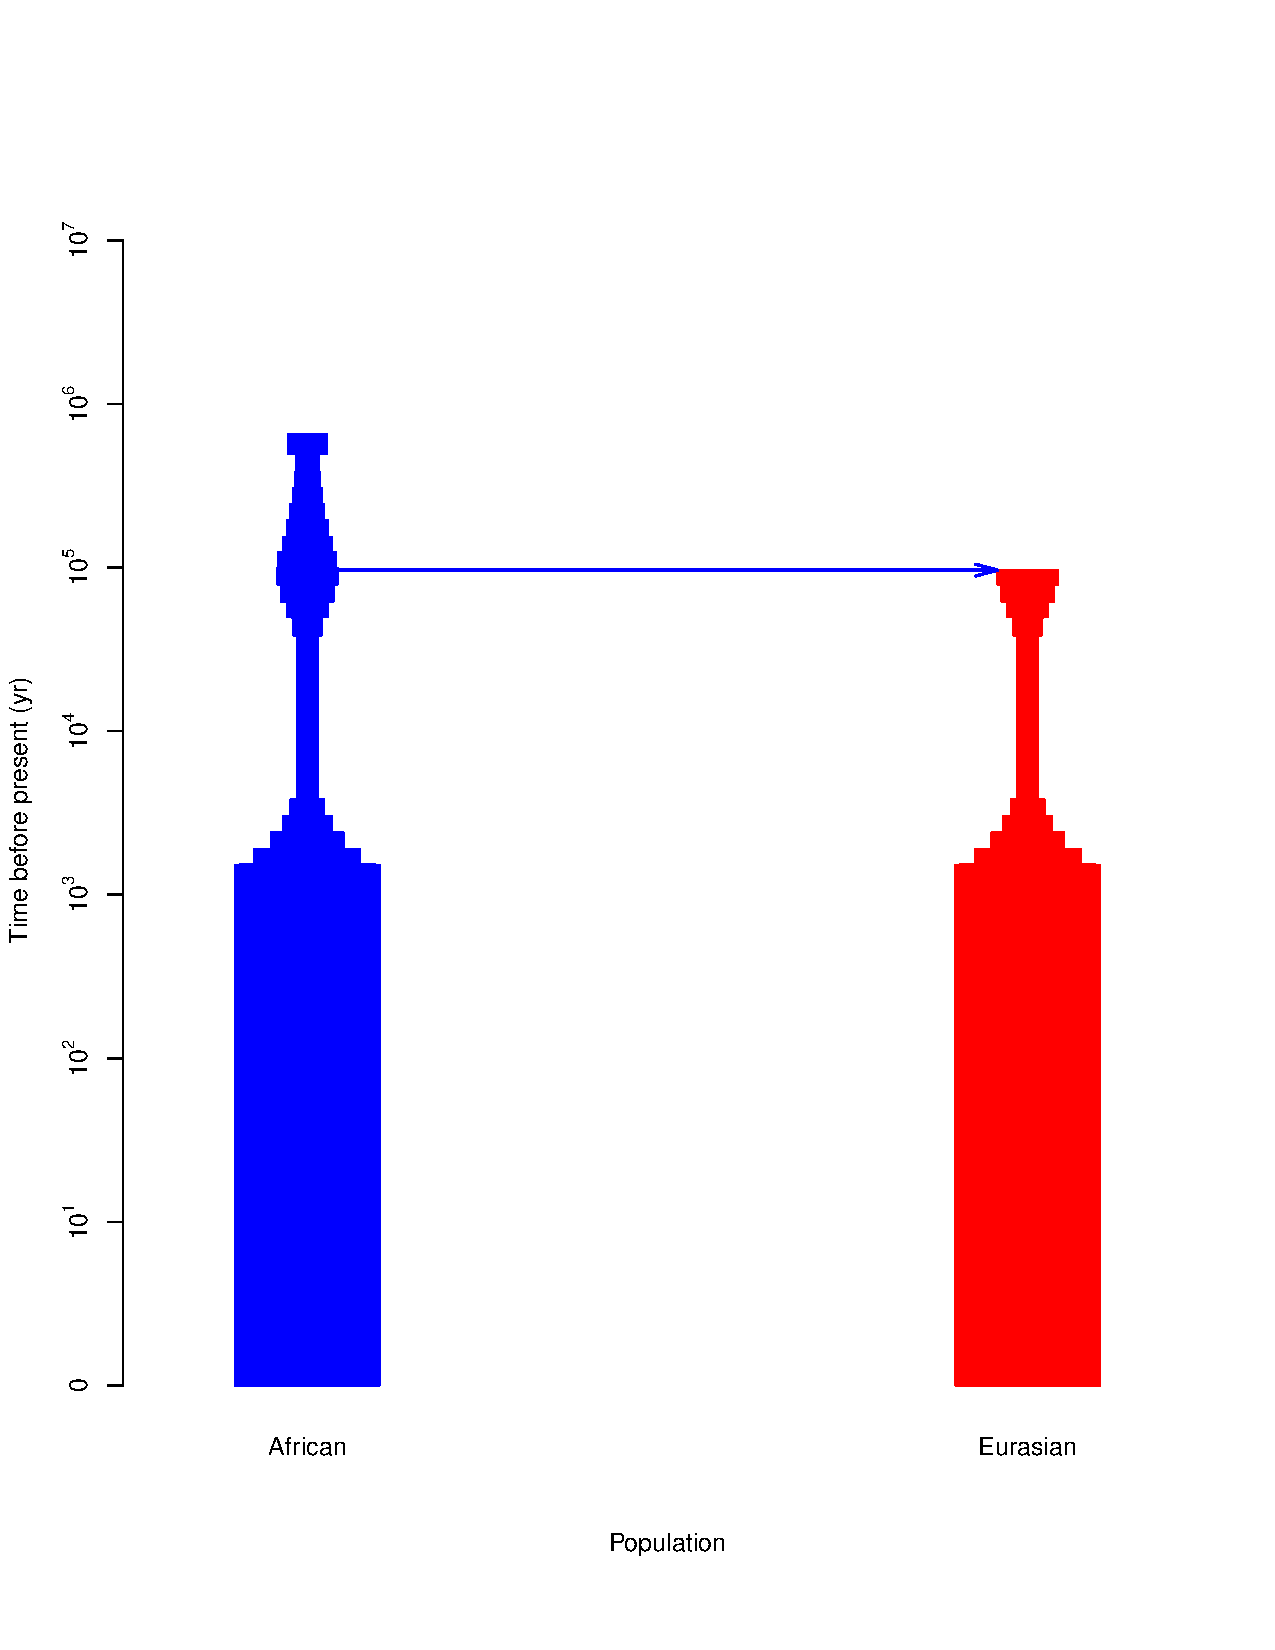
\includegraphics[width=0.5\textwidth]{plot/dem_smc2.pdf}
	\caption[SMCSMC seed demographic model]{Demographic model used as initialisation for SMCSMC analysis visualised using PopDemog \cite{Zhou2018}. The width of the coloured blocks represents the effective population size at that time.}
	\label{fig:smc2demog}
\end{figure}

Unless otherwise noted, the directionality of migration is given forwards in time. That is, from population A in the past to population B in the future. 


\subsection{Multiply Sequential Markovian Coalescent} We use MSMC2 to estimate the effective population size of pairs of African and Eurasian individuals using default configurations and scripts provided in {\tt msmc-tools} (see URLs) \cite{Schiffels2014, Wang2019a}. We use a fixed recombination rate in line with our SMCSMC analysis and skip ambiguously phased sites. Twenty iterations are performed by default. We additionally compute the relative cross-coalescent rate to examine relative gene flow by transforming the coalescent rates generated by MSMC2 as indicated in the software documentation.

A brief example is given below, where I estimate coalescence rates within population 1 (Eurasians), population 2 (Africans), and between them given properly formatted input. 

\begin{lstlisting}[language=Bash]
  msmc2 -I 0,1 --fixedRecombination --skipAmbiguous -t 1 -o {output_prefix} {input_string}
  msmc2 -I 2,3 --fixedRecombination --skipAmbiguous -t 1 -o {output_prefix} {input_string}
  msmc2 -I 0-2,0-3,1-2,1-3 --fixedRecombination --skipAmbiguous -t 1 -o {output_prefix} {input_string}
  python combineCrossCoal.py {input[2]} {input[0]} {input[1]} > {output[0]}
\end{lstlisting}

In order to convert between SMCSMC style input (seg files) and MSMC style input files, we use a custom script found \href{https://github.com/Chris1221/ancient_african_admixture/blob/master/pipelines/real_data/py/smc2-to-msmc.py}{here}.

\subsection{Inferring population size and migration rates in the Simons Genome Diversity Panel}

This section describes analysis of the SGDP with both SMCSMC and MSMC. SMCSMC version 1.0.1 was installed from the conda package manager (also found at \url{https://github.com/luntergroup/smcsmc/releases/tag/v1.0.2}), MSMC2 version 2.1.2 was installed from GitHub (found at \url{https://github.com/stschiff/msmc2/releases/tag/v2.1.2}) and all analyses were performed on the Oxford Biomedical Research Computation cluster. 

We download pre-phased sequencing data from \url{https://sharehost.hms.harvard.edu/genetics/reich_lab/sgdp/phased_data/} and mask for the strict accessibility mask from the 1000 genomes project. 
We additionally mask for any sites absent Chimpanzee ancestry due to a known issue with the phasing algorithm \cite{Wang2019a}. 
We perform this masking in {\tt vcftools}. We use the \gls{smc2} python package function {\tt smcsmc\.vcf\_to\_seg} to convert the sequence data from VCF to seg file format, a format very similar to MSMC format. 
Furthermore, we provide a script to convert from seg file format to MSMC file format as well. 
Unless otherwise noted, the names of individuals used in this paper are the first in their population (i.e. an individual named Yoruban is {\tt S\_Yoruba\-1} in the SGDP nomenclature, full list in \Cref{samples}).  
We select two diploid individuals from each population in Africa  and infer piece wise constant population size and directional migration rates. Specifically, we use the following options for SMCSMC:

\begin{lstlisting}[language=Bash]
smc2 -c -chunks 100 -no_infer_recomb -nsam 4 -I 2 2 2 -mu 1.25e-8 
  -rho 3e-9 -calibrate_lag 1.0 -EM \${EM} -tmax 3.5 -alpha 0.0 \
  -apf 2 -N0 14312 -Np ${Np} -VB ${DEMOGRAPHIC_MODEL} 
  -P 133 133016 31*1 -arg -o ${OUTPUT} -segs ${SEGS}
\end{lstlisting}

In order, we invoke the use of a QSUB cluster with {\tt -c} and split our analysis into 100 chunks. We do not infer recombination sites along with the demographic model in order to reduce runtime. Four haploid samples, two from each population, are analyzed with a fixed mutation rate of 1.25 $\times 10^{-8}$, a fixed recombination rate of 3 $\times 10^{-9}$, and accumulating events for one unit of survival time along the sequence. We use a given number of epochs for parameter units, and bound the upper limits of the trees at 3.5 times the effective population size (set to 14312). We use the look-ahead likelihood to guide the resampling process for a given number of particles {\tt Np} and use variational Bayes in place of the default stochastic expectation maximization algorithm. Parameters are inferred over 31 equally spaced intervals from 133 to 133016 generations in the past, and the sampled posterior ARGs are reported. The choice of these parameters is discussed in depth in \cite{10.1371/journal.pone.0247647}. 

The demographic model used to seed inference is given on page~\pageref{app:dem_model:seed}. We visualise this demographic model in the POPdemog package in \Cref{fig:smc2demog} \cite{Zhou2018}. This demographic model has been designed to roughly mimic human population size history without overly biasing the results from inference. 

Each SMCSMC analysis gives a final output file detailing migration and coalescent events, their rates, and their opportunities which denote the total opportunity for an event to occur during a particular epoch. Output files are trimmed to only visualise the final iteration of variational Bayes inference and assessed for convergence. Times and rates are interpreted differently than {\tt scrm} output. Rates are in units of $4N_0$ per generation (defined here as 29 years as per \cite{Fenner2005}), while times are given in generations. 

We implement the above in a {\tt Snakemake} pipeline. Sample size and relative cross-coalescent rates are transformed as described in the documentation using the same parameter values for mutation rate and generation time used for SMCSMC analysis.


Migration during the last 100ky is integrated into a metric we call the \gls{imf}. This is related to the cumulative migration fraction (CMF) as introduced in MSMC-IM \cite{Wang2019a}, except the quantity is integrated in a particular epoch. IMF is calculated as a function of time $F(t) = e^{- \int_{t=0}^T \rho(t) dt}$ given an upper bound $T$. A practically identical solution can be found from first principles. Consider $p$ proportion of the population are replaced every generation. Start with 0 individuals from the source $N_{source}$ population in the sink population $N_{sink}$, each generation replace $p$ proportion of the sink population with the source. We track the proportion of the population which are replaced by the source $P$.  


$$ \begin{aligned} P_0 &= 0 \\ P_1 &= pN_{sink} \\ P_2 &= pN_{sink} + p(N_{sink} - pN_{sink}) \\ &= pN_{sink} + pN_{sink}(1-p) \\ P_3 &= pN_{sink} + pN_{sink}(1-p) + p((N_{sink}-pN_{sink}) - p(N_{sink}-pN_{sink})) \\ &= pN_{sink} + pN_{sink}(1-p)+p(N_{sink}(1-p)-pN_{sink}(1-p)) \\ &= pN_{sink}+pN_{sink}(1-p)+pN_{sink}(1-p)(1-p) \\ &\dots \\ P_n &=N_{sink}p(1-p)^n \end{aligned} $$

In practice, both methods give essentially identical proportions for all considered questions. 

\begin{table}[ht]
    \centering
    \begin{tabular}{lll}
      \hline
    Name & ID & Source \\ 
      \hline
    French & S\_French-1 & SGDP \\ 
      Han & S\_Han-1 & SGDP \\ 
      Papuan & S\_Papuan-1 & SGDP \\ 
      BantuHerero & S\_BantuHerero-1 & SGDP \\ 
      BantuKenya & S\_BantuKenya-1 & SGDP \\ 
      BantuTswana & S\_BantuTswana-1 & SGDP \\ 
      Biaka & S\_Biaka-1 & SGDP \\ 
      Dinka & B\_Dinka-3 & SGDP \\ 
      Esan & S\_Esan-1 & SGDP \\ 
      Gambian & S\_Gambian-1 & SGDP \\ 
      Ju hoan North & S\_Ju\_hoan\_North-1 & SGDP \\ 
      Khomani San & S\_Khomani\_San-1 & SGDP \\ 
      Luhya & S\_Luhya-1 & SGDP \\ 
      Luo & S\_Luo-1 & SGDP \\ 
      Mandenka & S\_Mandenka-1 & SGDP \\ 
      Masai & S\_Masai-1 & SGDP \\ 
      Mbuti & S\_Mbuti-1 & SGDP \\ 
      Mende & S\_Mende-1 & SGDP \\ 
      Mozabite & S\_Mozabite-1 & SGDP \\ 
      Saharawi & S\_Saharawi-1 & SGDP \\ 
      Somali & S\_Somali-1 & SGDP \\ 
      Yoruba & S\_Yoruba-1 & SGDP \\ 
      Druze & HGDP00562 & HGDP \\ 
      Han & HGDP00774 & HGDP \\ 
      Karitiana & HGDP01013 & HGDP \\ 
      PapuanHighlands & HGDP00549 & HGDP \\ 
      PapuanSepik & HGDP00542 & HGDP \\ 
      Pathan & HGDP00224 & HGDP \\ 
      Pima & HGDP01043 & HGDP \\ 
      Sardinian & HGDP00670 & HGDP \\ 
      Yakut & HGDP00946 & HGDP \\ 
      Yoruba & HGDP00930 & HGDP \\ 
      San & HGDP01029 & HGDP \\ 
      Mbuti & HGDP00450 & HGDP \\ 
      Biaka & HGDP00460 & HGDP \\ 
      Vindija & Vindija.DG & Prufer et al. 2017 \\ 
      Altai & Altai\_published.DG & Pruefer et al. 2013 \\ 
      Denisovan & Deniosva\_published.DG & Myers et al 2012 \\ 
       \hline
    \end{tabular}
    \caption[Sample identifiers]{Sample IDs of the individuals used in this article and relevant resources.} 
    \label{samples}
    \end{table}
    

    \subsection{Statistical Analysis of Migrated Segments} \label{dstats_section}

    We run SMCSMC with the {\tt -arg} flag to report the posterior estimate of the ancestral recombination graph. We use this to isolate segments of the African genome where predicted migration events occurred between 50 and 70kya and used these segments to calculate drift statistics. The isolation procedure is implemented in {\tt smcsmc.find\_segments}, and involves sequentially reconstructing marginal trees and keeping track of which contain migration events in a particular epoch. We isolate segments from the marginal trees of all SGDP comparisons. 

\subsection{Length Distribution of Isolated Segments}


 Under the Markovian model of the SMC', the length of admixed tracts $L$ is an exponential process with scale factor $2N (1 - m ) \left( 1 - e^{-T / 2N} \right)$, with a proportion $m$ of the sink population being replaced with the source $T$ generations in the past and an effective population size of $N$ \cite{Marjoram2006,Liang953}. This gives an approximate mean length $\left[ (1 -m)r(T-1) \right]^{-1}$ with recombination rate $r$ in units of Morgans, which is well approximated
by  $(rT)^{-1}(1-m)$ \cite{Racimo2015}; we use this approximation to derive expected distribution of fragment sizes. When analysing populations with SMCSMC, we fix the recombination rate at $3 \times 10^{-9}$ uniformly across the genome, in line with that used by {tt MSMC} in simulations \cite{Schiffels2014}.
This value is a conservative underestimate, accounting for the presence of recombination hotspots and SMCSMC's inability to deconvolve recombinations in these areas, effectively underestimating the true $r$.  For estimates of ancestral tract lengths, we use the more universally accepted value of $1 \times 10^{-8}$, equivalent to a one percent chance of a cross-over per megabase and per generation \cite{Dumont2008}. 
%\todo{better reference for recombination rate value}


\subsection{Drift Statistics}

Patterson's drift statistics were calculated with {\tt ADMIXTOOLS} \cite{Patterson2012} and the {\tt admixr} package \cite{Petr2019} in {\tt R}. We converted the above sequence data to Eigenstrat format with {\tt vcf2eigenstrat} %\url{https://github.com/bodkan/vcf2eigenstrat} 
formerly distributed with {\tt admixr}. We merged SGDP and archaic Eigenstrat datasets with {\tt convertf} and {\tt mergeit} implemented in {\tt ADMIXTOOLS}. 

Here, Yoruba-1 is used as a representative of Western African groups, and used for ascertaining putatively migrated segments. Yoruba-2 is used as a comparison individual from the same populations. In this way, we look for evidence above another individual in the same population of similarity to Eurasians.

\subsection{Simulation procedure} \label{methods:simproc}

Coalescent simulations were performed under the sequential coalescent with recombination model ({\tt SCRM}) \cite{Staab2015}. 1 gigabase (Gb) of sequence was simulated.  In addition to branches in local genealogical trees, {\tt SCRM} retains non-local branches in the ancestral recombination graph (ARG) within a user-specified sliding window.  In the limit of a chromosome-sized windows {\tt SCRM} is equivalent to the coalescent with recombination, while for a zero-length window it is equivalent to the sequentially Markovian coalescent (SMC') \cite{McVean2005,Marjoram2006}; we use a $100$kb sliding window to approximate the CwR and improve accuracy over SMC' while retaining tractable inference.

We modelled migration as a 10ky pulse of constant migration rate resulting in an integrated migration fraction (IMF) of 0 to 0.593. The migration pulse was centered at various times between 40 and 70 kya.  Due to the amount of compute required, we then used SMCSMC to infer the demographic parameters using a reduced set of 5000 particles and 5 iterations of the VB procedure. To aid convergence, we started inference at a reasonable approximation of human demographic history (\Cref{fig:dem}). We modelled $N_e$ and migration rates as piece-wise continuous functions and set 32 exponentially spaced epochs from 133 to 133016 generations in the past. To convert evolutionary rates to years we set a generation time of 29 years \cite{Fenner2005}.  For computational efficiency, individual genomes were split into 120 chunks and processed in parallel, with sufficient statistics collected and processed together in the VB steps.


\begin{figure}[hb]
  \centering
  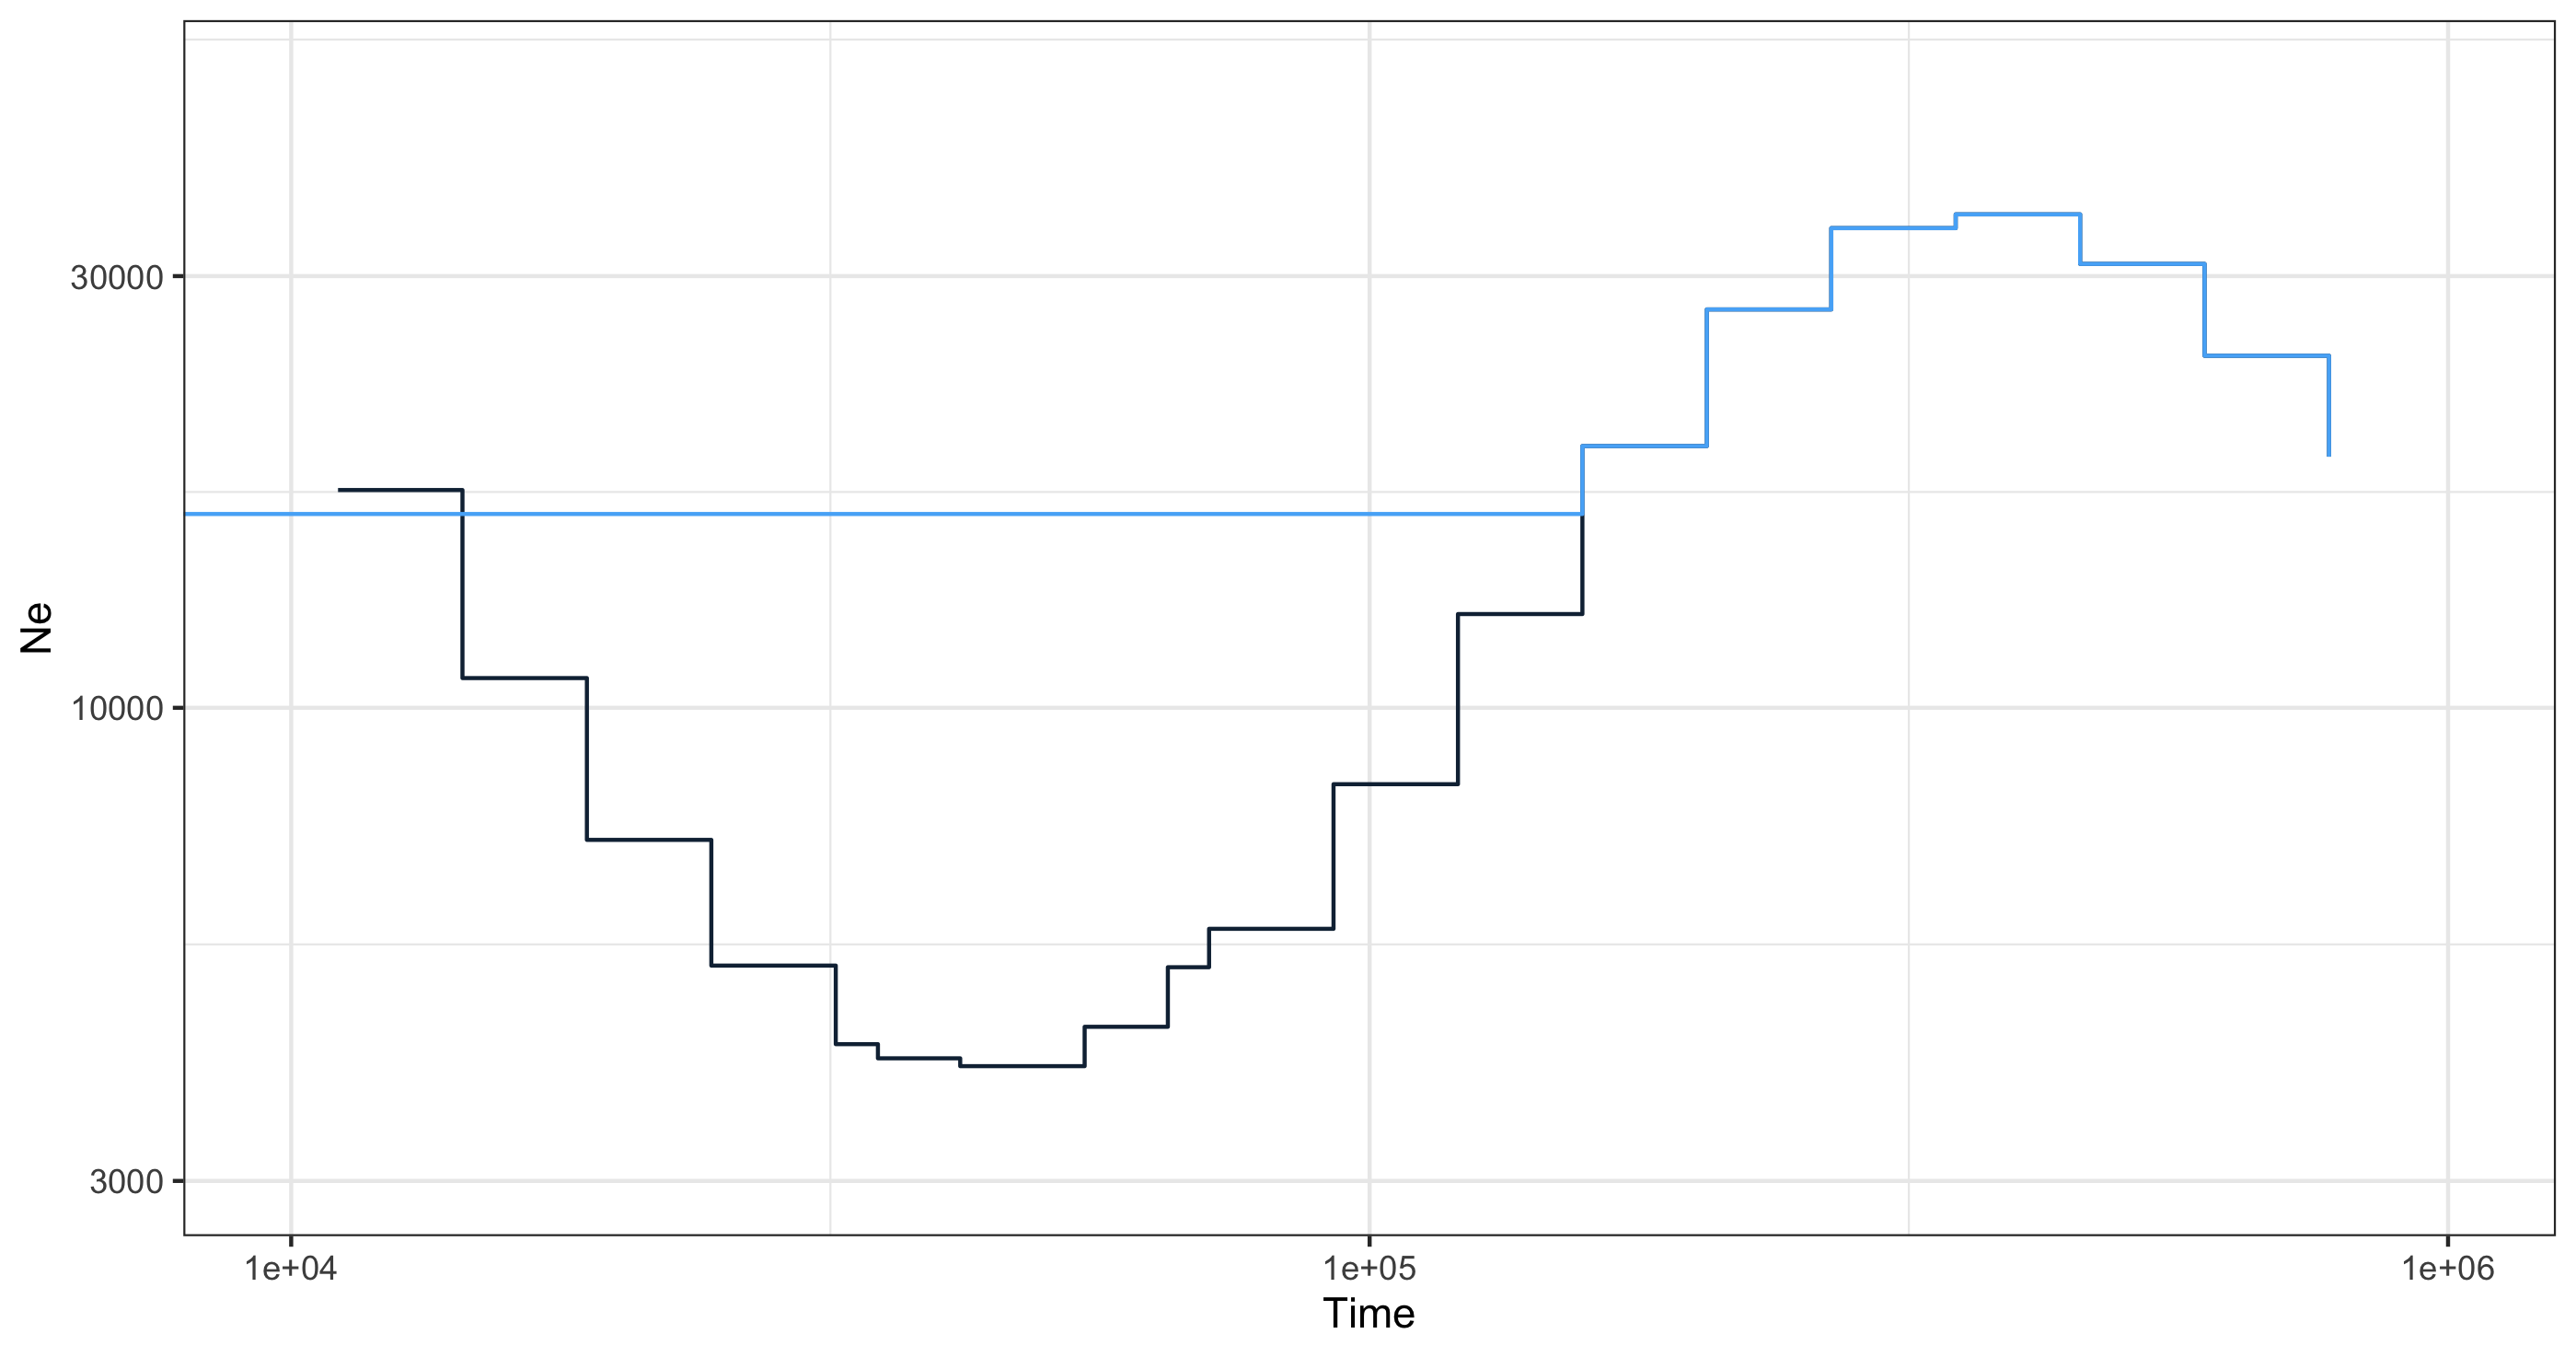
\includegraphics[width = 0.5\linewidth]{plot/demographic_model.png}
  \slcaption{Effective Population size model used for simulations. Following the simulation procedure in \Cref{methods:simproc}, the population size model is plotted per epoch, with the effectively African population plotted in blue and the effectively non-African population in black. }
  \label{fig:dem}
\end{figure}

Times are in units of $4N_0g$ while population sizes are in units of $N_0$. For $g=29, N_0 = 14312$, the demographic model is as shown in \Cref{fig:dem}.  Exact specifications are given in \Cref{app:dem_model}

The demographic model which we have assumed for both population's effective sizes has been shown to recapitulate similar inference to real data (data not shown). The migration parameter must be initiated at a given magnitude; further back in time, the particle filter is less able to identify lineage's true populations, and the inference of migration rates becomes essential uniform. Thus, we see a ``drop-off'' effect, where in the ancient past, the inference remains at the initiation value, and as more certainty about different histories is obtained, the migration values recapitulate real information. Thus, the choice of an appropriate parameter for the initial migration rate is a crucial step in SMCSMC analysis, and here we chose to arrive at this value through simulation.

We simulate back-migration scenarios of varying total migration proportions from 0 (no migration) up to 60\% population replacement. For each simulation, we initiate the particle filter at either 0, 1, or 5 units of $\frac{1}{4 N_0}$ proportion replaced per generation (which are the units used internally by {\tt scrm} and {\tt ms} for simulation).  SMCSMC is then used to infer effective population size and migration histories in five iterations with 5000 particles. As a cautionary note, these simulations are almost certainly not fully converged, and are used as an indication of power. However, these low resolution attempts are indicative of a ``quick'' overview of the abilities of the algorithm. With 600 cores available, each of the cases (forward, backward, or bidirectional) was able to run in approximately 20 hours. 

Generally, beginning with a higher migration rate seems to recover a higher proportion of the simulated migration. However, as in the case of a 60\% replacement simulated 40kya, beginning with 5 4$N_0$ rather than 1 4$N_0$ recovers similar proportions of backwards migration (0.502 vs 0.52) yet the higher migration rate finds 0.301 Eurasian migration rather than 0.195. The higher initial migration rates thus slightly reduce power (though, not in all cases, and for fully converged solutions, we would expect both proportions to be similar up to noise) while additionally finding an increased migration in the opposite direction.  Beginning with a zero rate leads to highly unstable estimates of the migration rate and effective population size, and we exclude it from our analysis.




\subsection{Isolating Anciently Admixed Segments} 


To investigate shared genetic drift in sequences putatively inherited from an ancient migration, we study a single sample from the posterior in detail. We sample genealogical trees with migration events from the posterior distribution estimated by the particle filter under the final, converged, demographic parameters.  With the caveat that no single instance of an evolutionary history will be definitively ``true'', inferred coalescence and migration events within inferred marginal trees are representative of the underlying demographic processes \cite{Hubisz2020}. This makes individual events in segments of the genome good candidates for analysis in aggregate. 
We scan along the sequence and identified marginal trees with migration events from the source (Eurasian) population to the sink (African) population (forward in time) within the desired time period along with the beginning and end position of that tree in the genome sequence. In this process, we ignore recombination events that alter a tree in such a way that the migration event is retained.  

\subsection{Sequence Data and Preparation}  We downloaded whole genome sequence (WGS) data from the phased release of the Simons Genome Diversity Panel and converted it to {\tt .seg} file format using scripts provided (See URLs). We apply two masks to the data. First, we mask the data with the strict accessibility mask provided by the 1000 genomes project (see URLs). Second, we mask any sites absent chimpanzee ancestry, to address a known variant issue in the data that resulted in artificially long runs of homozygosity \cite{Wang2019a}. We develop a {\tt Snakemake} \cite{Koster2012} pipeline for efficiently analysing sequence data with both SMCSMC and MSMC2. We assume a mutation rate of $1.25\times10^{-8}$ and a recombination rate of $3\times10^{-9}$ (events per nucleotide per generation), in line with recent literature \cite{Scally2012, Schiffels2014a}. The number of particles, and the number of VB iterations, are set per analyses, and are reported in figure captions. Unless otherwise noted, the names of individuals used in this paper are the first in their population (e.g.\ an individual named Yoruban is {\tt S\_Yoruba-1} in the SGDP nomenclature); a complete list of sample identifiers is provided in \Cref{samples}. 



\subsection{Integrated Migration Fraction}
The IMF, the total fraction of a particular population $A$ replaced during a particular time period from $T_0$ to $T_1$ generations in the past is found as follows. Let $\rho(t)$ be the instantaneous rate of migration out of $A$ per unit of time in the backward direction (i.e.\ into $A$ forwards in time), and $F(t)$ the fraction not migrated in the epoch $[T_0,t]$, then $\frac{d}{dt} F(t) = -\rho(t) F(t)$ with solution $F(t) = e^{- \int_{T_0}^{T_1} \rho(t) {\mathrm{d}t}}$, so that the IMF is given by $1-F(T_1)$.  The integral is calculated as a finite sum since $\rho$ is piece-wise constant.




\section{Results}

\subsection{Substantial Migration from Eurasian to African Ancestors} We use SMCSMC to analyse pairs of individuals from the SGDP and simultaneously infer migration rates and effective population sizes ($N_e$) under a two-island model with directional migration.  Population sizes and migration rates are modeled as piece-wise constant across 32 exponentially spaced epochs from 133 to 133016 generations in the past, corresponding to 3.8 thousand to 3.8 million years ago (3.8kya--3.8Mya) using a generation time $g=29$ years \cite{Fenner2005}.  We find that the method infers high rates of migration from descendants of the OoA event ('non-Africans') to Africans, but not in the opposite direction, in the period $30$--$70$kya corresponding to the Late Middle Paleolithic (\Cref{fig:migrationplot}). In populations from the Niger-Kordofanian and Nilo-Saharan language groups, comprising the majority of the population on the African continent, the peak inferred migration rate from Eurasian populations ($2.5$--$3.0\times 10^{-4}$ and $3.5$--$4.0\times 10^{-4}$, in units of proportion of the target (ancestral African) population replaced per generation) most frequently falls in the epochs spanning 35--45kya, while peak migration rates in the opposite direction are substantially lower ($0.5$-$1.0\times 10^{-4}$) and occur earlier, in the epochs spanning $55$--$70$kya (\Cref{fig:peaks}). Populations in the Afroasiatic language group show evidence of large amounts of directional migration in the Holocene (\Cref{fig:sgdp_mig}), which is consistent with previous findings of relatively recent European introgression into these populations \cite{Busby2016, Fan2019}. 

%Inferred migration varies across language groups (\Cref{fig:migrationplot}, \Cref{table:sgdp_pairwise}). Afroasiatic groups show high migration from Han and French populations, with a lower proportion deriving from Papuans. Niger-Kordofanian and Nilo-Saharan groups show an intermediate magnitude, between 50 and 60 percent replacement, though also significantly (P < 0.05, two-tailed paired $T$ test) closer to French and Han sources than Papuans. The Khoesan show the lowest migration, consistent with their early diversification from the remainder of African groups and the relative lack of gene-flow from Western African populations \cite{Lipson2019}. This is contrasted with the Mbuti and Biaka, Central African Hunter Gatherer populations who have historically received substantial amounts of gene flow from Western African sources. Both of these populations show the lowest migration in their language group (\Cref{average_sgdp_migration_table}).  

\begin{table}[ht]
  \centering
  \begin{tabular}{llrr}
    \hline
  Language Family & Comparison Family & Mean Difference (95\% CI) & Adjusted P \\ 
    \hline
  Niger-Kordofanian & Nilo-Saharan & -0.053 (-0.081--0.025) & 1.11e-03 \\ 
    Niger-Kordofanian & Khoesan & 0.143 (0.125-0.161) & 4.39e-14 \\ 
    Niger-Kordofanian & Afroasiatic & -0.125 (-0.142--0.107) & 1.67e-15 \\ 
    Nilo-Saharan & Niger-Kordofanian & 0.053 (0.025-0.081) & 1.11e-03 \\ 
    Nilo-Saharan & Khoesan & 0.196 (0.169-0.223) & 6.91e-09 \\ 
    Nilo-Saharan & Afroasiatic & -0.072 (-0.098--0.045) & 1.23e-04 \\ 
    Khoesan & Niger-Kordofanian & -0.143 (-0.161--0.125) & 4.39e-14 \\ 
    Khoesan & Nilo-Saharan & -0.196 (-0.223--0.169) & 6.91e-09 \\ 
    Khoesan & Afroasiatic & -0.268 (-0.284--0.252) & 3.62e-13 \\ 
    Afroasiatic & Niger-Kordofanian & 0.125 (0.107-0.142) & 1.67e-15 \\ 
    Afroasiatic & Nilo-Saharan & 0.072 (0.045-0.098) & 1.23e-04 \\ 
    Afroasiatic & Khoesan & 0.268 (0.252-0.284) & 3.62e-13 \\ 
    CAHG & Niger-Kordofanian & -0.084 (-0.119--0.049) & 1.18e-03 \\ 
     \hline
  \end{tabular}
  \caption[Tests for significance between integrated migration fractions within African populations in the SGDP]{ Differences in African IMF in the SGDP. The integrated migration fraction (IMF) in the epoch 30--70kya is calculated as per the Methods section for all comparisons in the Simons Genome Diversity Project (SGDP), and a two tailed $t$-test is used to statistically test for differences between the inferred migration in African language groups. Averaged over three technical replicates to account for the influence of stochastic sampling variation. P values corrected for multiple testing using the Bonferroni method. Abbreviations: CAHG, Central African Hunter-Gatherers (include Mbuti and Biaka); CI, Confidence Interval.} 
  \label{table:sgdp_pairwise}
  \end{table}


\begin{table}[ht]
\centering
\begin{tabular}{llll}
  \hline
Language Family & Partner Population & Mean AFR IMF (SD) & Mean EUR IMF (SD) \\ 
  \hline
Afroasiatic & All & 0.477(0.015) & 0.176(0.038) \\ 
  Afroasiatic & French & 0.477(0.006) & 0.207(0.044) \\ 
  Afroasiatic & Han & 0.492(0.01) & 0.168(0.032) \\ 
  Afroasiatic & Papuan & 0.462(0.011) & 0.153(0.024) \\ 
  Khoesan & All & 0.209(0.013) & 0.044(0.006) \\ 
  Khoesan & French & 0.217(0.007) & 0.051(0.003) \\ 
  Khoesan & Han & 0.217(0.002) & 0.042(0) \\ 
  Khoesan & Papuan & 0.193(0.006) & 0.04(0) \\ 
  Niger-Kordofanian & All & 0.352(0.04) & 0.088(0.017) \\ 
  Niger-Kordofanian & French & 0.36(0.039) & 0.102(0.015) \\ 
  Niger-Kordofanian & Han & 0.363(0.04) & 0.083(0.013) \\ 
  Niger-Kordofanian & Papuan & 0.334(0.038) & 0.078(0.013) \\ 
  Nilo-Saharan & All & 0.405(0.033) & 0.107(0.016) \\ 
  Nilo-Saharan & French & 0.414(0.037) & 0.123(0.016) \\ 
  Nilo-Saharan & Han & 0.417(0.036) & 0.106(0.01) \\ 
  Nilo-Saharan & Papuan & 0.385(0.029) & 0.093(0.008) \\ 
   \hline
\end{tabular}
\caption[Tests for difference between integrated migration fractions in the SGDP averaged over African language families]{Integrated Migration Fraction (IMF) in either direction averaged over African language groups. SMCSMC was used to infer directional migration and effective population size between populations in the Simons Genome Diversity Project. The total migration between each African and non-African population was integrated in the epoch 30--70kya (see Methods) and averaged over language family. Abbreviations: Integrated Migration Fraction (IMF), Standard Deviation (SD), EUR (Eurasian), AFR (African)} 
\label{table:average_sgdp_migration_table}
\end{table}

  

We track the overall peak of migration rate in different populations (\Cref{fig:peaks}a,b). The most common backwards migration peak falls in the epoch between 35--45kya in the Nilo-Saharan and Niger-Kordofanian groups. Forwards migration has an earlier peak, in the epoch spanning 55--70kya. This result must be interpreted in light of the simulation results presented below.  

We model the migration adjusted $N_e$ in Eurasian populations, averaged over African partners, and African populations averaged over Eurasian partners (\Cref{fig:individual_pop_sizes}). The resulting curves largely represent our prior knowledge of world history, with an early divergence of Papuans consistent with the timing proposed in \cite{Malaspinas2016}, and a second bottleneck of populations inhabiting North America such as the Karitiana and Pima. Because we do not explicitly infer population split times, and there is no clear summary metric as proposed by MSMC2 in the case of directional migration, more fine-scale trends are difficult to identify. The African population size models show more discrepancy between populations, including an OoA-like bottleneck in Afroasiatic populations, and a large historical population size in hunter-gatherer groups such as proposed in \cite{Lipson2019}. 


\begin{figure}
	\centering
	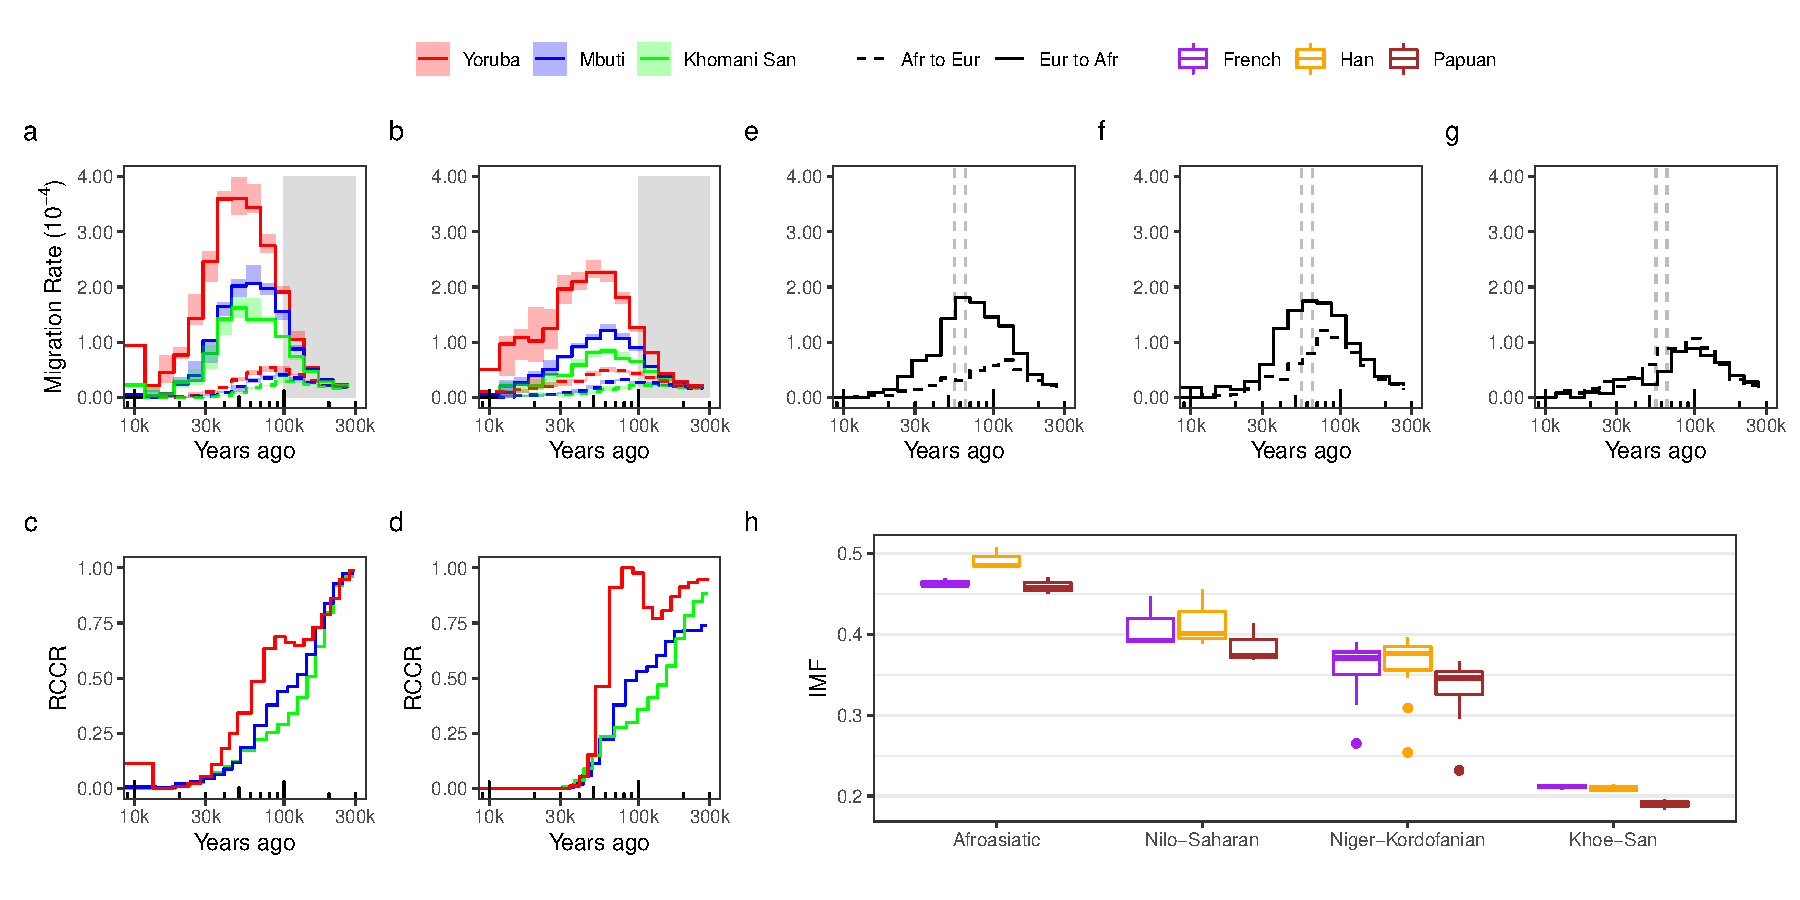
\includegraphics[width=\textwidth]{plot/new_mig_plot.pdf}
	\caption[SMCSMC finds directional migration from the ancestors of Eurasians to the ancestors of Africans]{Migration rate inference. {\bf a}. Inferred migration between an African individual and a Han Chinese individual in the SGDP. Three replicates were performed, with the median estimate plotted and the range shaded. Solid lines show inferred migration from Eurasians to Africans (forward in time) while dotted lines show the reverse migration. The SMCSMC analysis used 10000 particles to estimate the posterior distribution of marginal trees, and 25 iterations of variational Bayesian inference to achieve converged parameter estimates. The shaded grey regions represent a time period where simulation shows SMCSMC has very little power to infer migration (details found in \Cref{methods:simproc}).  {\bf b}. The same analysis as in a. except using individuals from the physically phased subset of the HGDP, showing similar differences between populations but systematically lower migration overall. Three replications were performed to estimate error and the standard deviation is shaded. The same SMCSMC settings were used as in a. {\bf c}. Relative cross-coalescence rate (RCCR) estimated by MSMC in three different populations in the SGDP, supporting gene flow between Eurasians and Yorubans not shared by Mbuti or Khoe-San. 40 iterations were used to achieve parameter convergence. {\bf d}. The same analysis as in c. but performed on individuals in the physically phased subset of the HGDP, similarly supporting shared gene flow between the Yoruban and Eurasians not shared by Mbuti or Khoe-San. {\bf e}, {\bf f} and {\bf g}. Inferred migration rates from data simulated under a two-island model with, from left to right, a backward Eurasia-to-Africa, a bidirectional, and a forward migration pulse lasting 10 ka BP (dashed vertical lines) and replacing 40\% of the recipient population(s) approximately 60kya. The migration rate from Africa to Eurasia is not well estimated by SMCSMC (\Cref{fig:backsim}--\Cref{fig:fwdsim} and \Cref{methods:simproc}), but SMCSMC is well powered to infer migration from Eurasia to Africa in this period. {\bf h}. Integrated total migration fraction (IMF) over the last 100 thousand years stratified by language phyla in the SGDP and comparison Eurasian population used to estimate migration. Afroasiatic (Mozabite, Saharawi, and Somali), Nilo-Saharan (Dinka, Luo, and Masai), Niger-Kordofanian (BantuHerero, BantuKenya, BantuTswana, Biaka, Esan, Gambian, Luhya, Mandenka, Mbuti, and Mende), and San (Khomani San and Ju hoan North) are grouped as in \cite{Fan2019}. Similar levels of migration are inferred from French and Han Chinese to all language groups, with significantly less migration from Papuan groups ($p\leq 0.05$, two-tailed paired t-test, \Cref{table:average_sgdp_migration_table}). Outliers in the Niger-Kordofanian group are the Mbuti. }
	\label{fig:migrationplot}
\end{figure}

\begin{figure}[h]
  \centering
  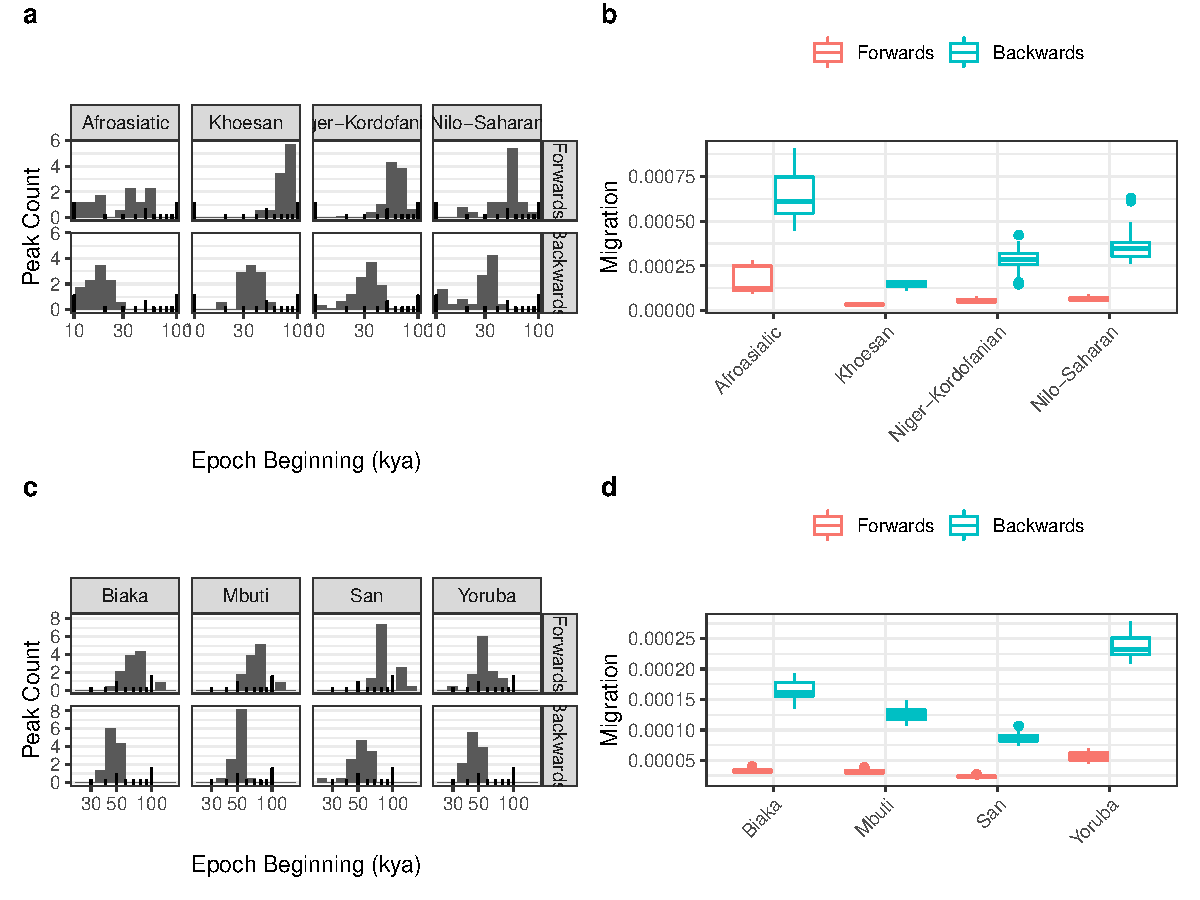
\includegraphics[width=\textwidth]{plot/peaks.pdf}
  \caption[Timing and average maximum rate of directional migration in HGDP and SGDP]{Timing and average maximum rate of directional migration in HGDP and SGDP. {\bf a} Migration is inferred in evenly spaced epochs on the log scale from 3.8 thousand to 3.8 million years ago. For each population in the SGDP, we record the epoch with the highest inferred directional migration rate (the ``peak'' of migration) and plot this as a histogram. Backwards migration refers to migration from Eurasians to Africans, whilst forward represents the reverse. {\bf b} In the epochs of highest migration identified in a., we record the inferred rate per population and plot these as a boxplot. Whiskers represent 1.5 times the interquartile range. The migration rate is given in proportion of the population replaced per generation. {\bf c} and {\bf d} represent the same analyses as in a. and b. calculated for the Human Genome Diversity Panel, rather than the SGDP.}
  \label{fig:peaks}
\end{figure}

\begin{figure}
	\centering
	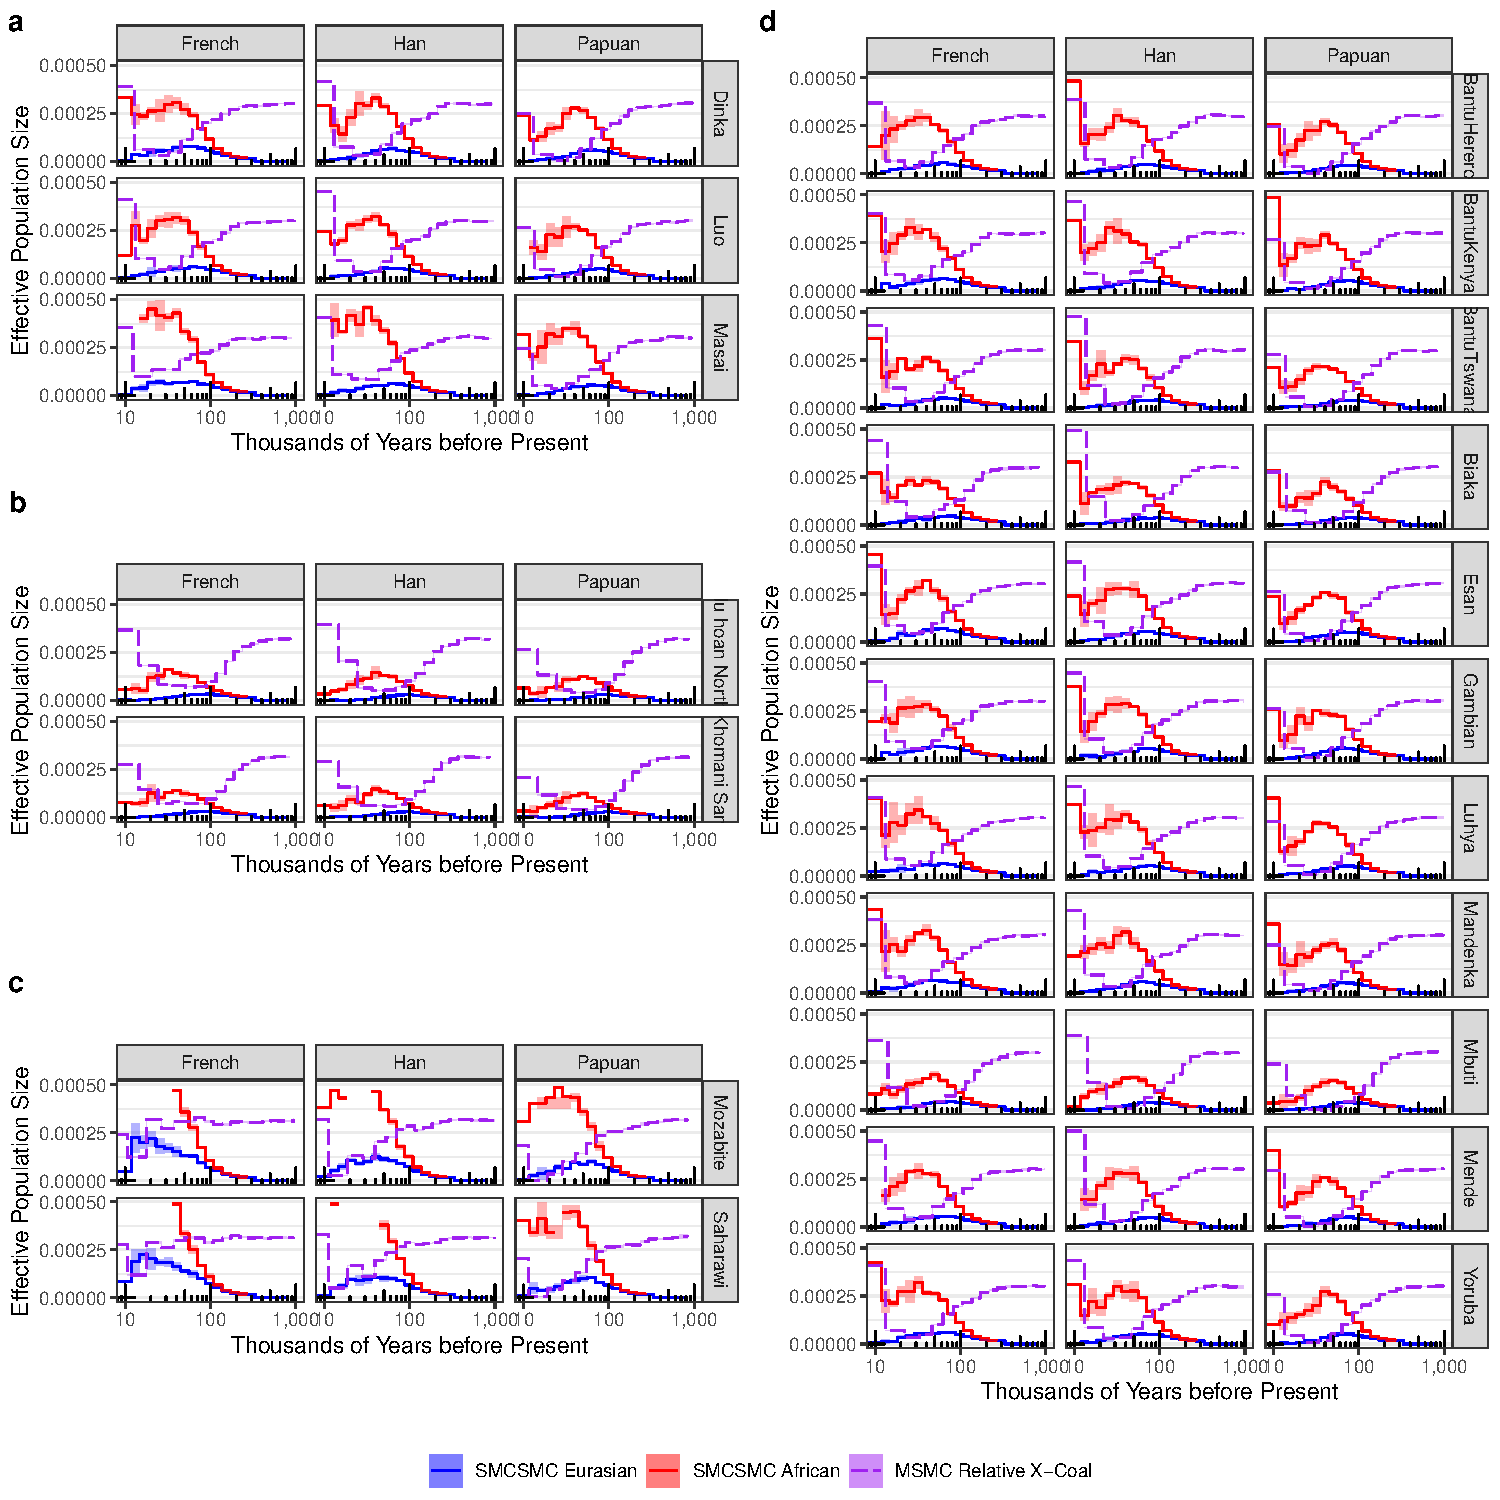
\includegraphics[width=0.95\linewidth]{plot/sgdp_mig_new.pdf}
	\caption[Full directional migration inference results from SGDP]{{\bf Inference of directional migration in the Simons Genome Diversity Project.} The SMCSMC particle filter was used to infer directional migration rates in both directions from one of three Eurasian populations (French, Han, and Papuan) to one of 18 African populations. 5000 particles were used to approximate the ancestral recombination graph with 10 iterations of variational Bayesian inference to update demographic parameter values. Panels represent a. Nilo-Saharan, b. KhoeSan, c. Afroasiatic, and d. Niger-Kordofanian language families. Alongside the SMCSMC inference, we use MSMC2 to infer the relative cross coalescent rate (RCCR) with default settings and 20 iterations for convergence.}	
	\label{fig:sgdp_mig}
\end{figure}


To assess the impact of errors introduced by statistical phasing, as is the case for the SGDP, we repeated the analyses above on a subset of physically phased individuals from the Human Genome Diversity Project (HGDP) \cite{Mallick2016} 


\subsection{Validation in a physically phased subset of the Human Genome Diversity Panel (HGDP)} \label{hgdp_section}

Phased data is not essential for demographic inference using SMCSMC; however, the use of phase alongside the look-ahead likelihood allows for more efficient convergence. The Human Genome Diversity Project collected 929 genomes from a diverse collection of human populations \cite{Bergstrom2019}. 36 of these genomes, two each from nine Eurasian and four African populations, were physically phased by use of linked-read sequencing technologies. This resource allows us to validate our inference both in an independent dataset, and evaluate the effect of phasing errors on SMCSMC inference.   

To analyse these data, the same {\tt Snakemake} pipeline was used with minor adjustments in wildcard constrains to account for differences in sample names. 120 chunks of the genome were run in parallel for reasons of computational efficiency, while fixed recombination rate and mutation rates were held at the same values as the SGDP analysis, and an identical demographic model was used to initiate the analysis. Three replicates of the analysis were performed to assess the impact of stochastic sampling variation on inference. We infer both effective population size and directional migration in each of these 9x4 comparisons between Eurasian and African populations (\Cref{fig:both}a). The resulting inference allows us to verify and validate many observations from the SGDP.

Firstly, we calculate the timing of the migration peak and its magnitude, and find the estimates largely in line with the SGDP inference (\Cref{fig:peaks}c,d). For instance, inferred backwards migration in the Yoruban and Biaka populations peak at 40-50kya, while the Mbuti and San show earlier migration peaks around 50-60kya (\Cref{fig:peaks}c). The migration rate at the peak shows the same qualitative trends as the SGDP, with the peak in the Yoruban (approximately $2.5\times10^{-4}$) far exceeding the peaks in the Biaka, Mbuti, or San (between $0.1-0.175\times10^{-4}$) (\Cref{fig:peaks}d). This replication in the HGDP confirms the presence of a large directional migration in the Late Middle Pleistocene, and demonstrates that statistical errors in phasing the SGDP are not large contributors to the qualitative trends observed. 

We integrate migration between 40--70kya to obtain the inferred IMF for each of the comparisons in the HGDP (\Cref{fig:both}b). Differences amung the African populations mirror those in the SGDP, though the proportions are uniformly smaller (main text). However, the migration rates backwards into Africa are apparent in all comparisons, and the order of populations IMF remains the same. Differences between individual Eurasian donor populations are small and, with the exception of the Papuan, insignificant. A discussion of the Papuan comparisons appears in the subsequent section.  

To compare the HGDP inference with the SGDP inference, we construct a set of the SGDP with the same donor populations as the HGDP.



%For the SMCSMC algorithm, the use of phased data is not necessary but does help with efficient convergence by assisting the lookahead-likelihood-guided resampling. Therefore, we do not expect errors made during statistical phasing to significantly impact the inferred parameters. However, to test this, we replicate the above analysis in a physically phased subset of the HGDP downlaoded from \url{ftp://ngs.sanger.ac.uk/production/hgdp/hgdp_wgs.20190516/}. The same {\tt snakemake} pipeline is used as in the analysis of the SGDP data. Data is additionally masked for the filters provided with the data. 

%We first asked if we could replicate the inflated African $N_e$ estimates from the main text in this new, high quality, data set. To do this, we infer effective population size with SMCSMC and MSMC.  The full inference from both algorithms is shown in \Cref{fig:hgdp_ne} and \Cref{fig:hgdp_mig}. For SMCSMC, we use 10,000 particles and 15 iterations to achieve convergence, with the same recombination and mutation rates as in the SGDP analysis.  The source populations here are more diverse than in the main text, comprising a sample of global diversity including Druze, Han, Karitiana, two Papuans, Pathan, Pima, Sardinians, and Yakut. To obtain a comparable sample from the SGDP, we select populations matching those in the HGDP. We match each of the source and sink populations, and similarly infer their effective population size and migration histories. The full inference is shown in \Cref{hgdp_sgdp_ne} and \Cref{fig:hgdp_sgdp_mig}.


\subsection{Comparisons between the HGDP and a subset of the SGDP}

Previously, inference in the SGDP has relied on three candidate Eurasian donor populations. However, the physically phased subset of the HGDP provides a higher resolution view into global migration patterns with nine Eurasian populations represented. In order to compare effectively between the inferences made in these two datasets, we find representatives from these nine Eurasian populations in the SGDP dataset and use them as donor populations to the same four African populations (Yoruban, San, Mbuti, and Biaka), effectively recreating the analysis done in the physically phased subset of the HGDP. We select the Khomani San as a representative of the San, and only use one of the Papuan populations in the HGDP to compare (Highlands, as opposed to Sepik), creating the same 8x4 analysis table for both data sets. We infer the effective population sizes and migration rates using both SMCSMC and MSMC, with analysis details effectively identical to the original comparisons listed above (\Cref{fig:hgdp_sgdp}). We average over inferences to visually compare trends between the two datasets, in the same populations and compute the inferred IMF between 40--70kya (\Cref{fig:both}).  

In both the HGDP and the SGDP, MSMC estimates of African population size are higher than SMCSMC estimates in the ancient past (80 -- 300kya) (\Cref{fig:both}a). By modelling directional migration, we are able to account for excess genetic diversity in the ancestral African population in both datasets. Uncertainty in the estimates increases substantially nearer to the present, as would be expected with the SMCSMC method. 

We summarise migration from 40--70kya in the HGDP similarly to the SGDP. The total inferred migration is lower in the HGDP than in the SGDP (\Cref{fig:both}b). We use this comparison setup to additionally test the differences between Papuan donors and the remainder of Eurasians. We construct a linear model predicting IMF based on an indicator variable of Papuan/not Papuan and the receptor donor population, and find that in both the SGDP and the HGDP, Papuans show approximately 2\% less IMF than other donor populations (\Cref{table:hgdp:papuan_imf}, \Cref{table:sgdp:papuan_imf}). While this difference is small, it is highly significant. However, the demographic scenario causing this difference in inferred IMF is not obvious; it is possible that the Papuan group had begun to diverge from the donating population prior to the admixture event, or alternatively that differences in archaic admixture between Eurasian and Papuan groups make up the difference in affinity. 



However, the qualitative patterns in inferred directional migration rates between populations are similar in both datasets (\Cref{fig:both}c). In both datasets, the highest rates are found in the Yorubans, follow by the Biaka, then the Mbuti and San. The MSMC curves are interestingly dissimilar between the different data sets, with a much steeper ascent around the period of our inferred migration in the HGDP than the SGDP. 



%This data set comprises individuals from four African (Yoruban, San, Mbuti, and Biaka) and nine non-African populations (Druze, Han, Karitiana, two Papuan populations, Pathan, Pima, Sardinian, and Yakut). SMCSMC results in the HGDP are qualitatively similar to those in the SGDP (\Cref{fig:migrationplot}b, \Cref{fig:peaks}a). Inferred migration rates are, in general, lower in HGDP data than when using matched SGDP samples (\Cref{fig:migrationplot}a,b and \Cref{fig:both}, demographic inference in matched sampled in \Cref{fig:hgdp_sgdp}), but in all cases, the migration rates from Eurasia to Africa are substantially higher than in the opposite direction, consistent with the findings in the SGDP (Supplemental Fig.\ \Cref{fig:both}). 

\begin{figure}
  \centering
  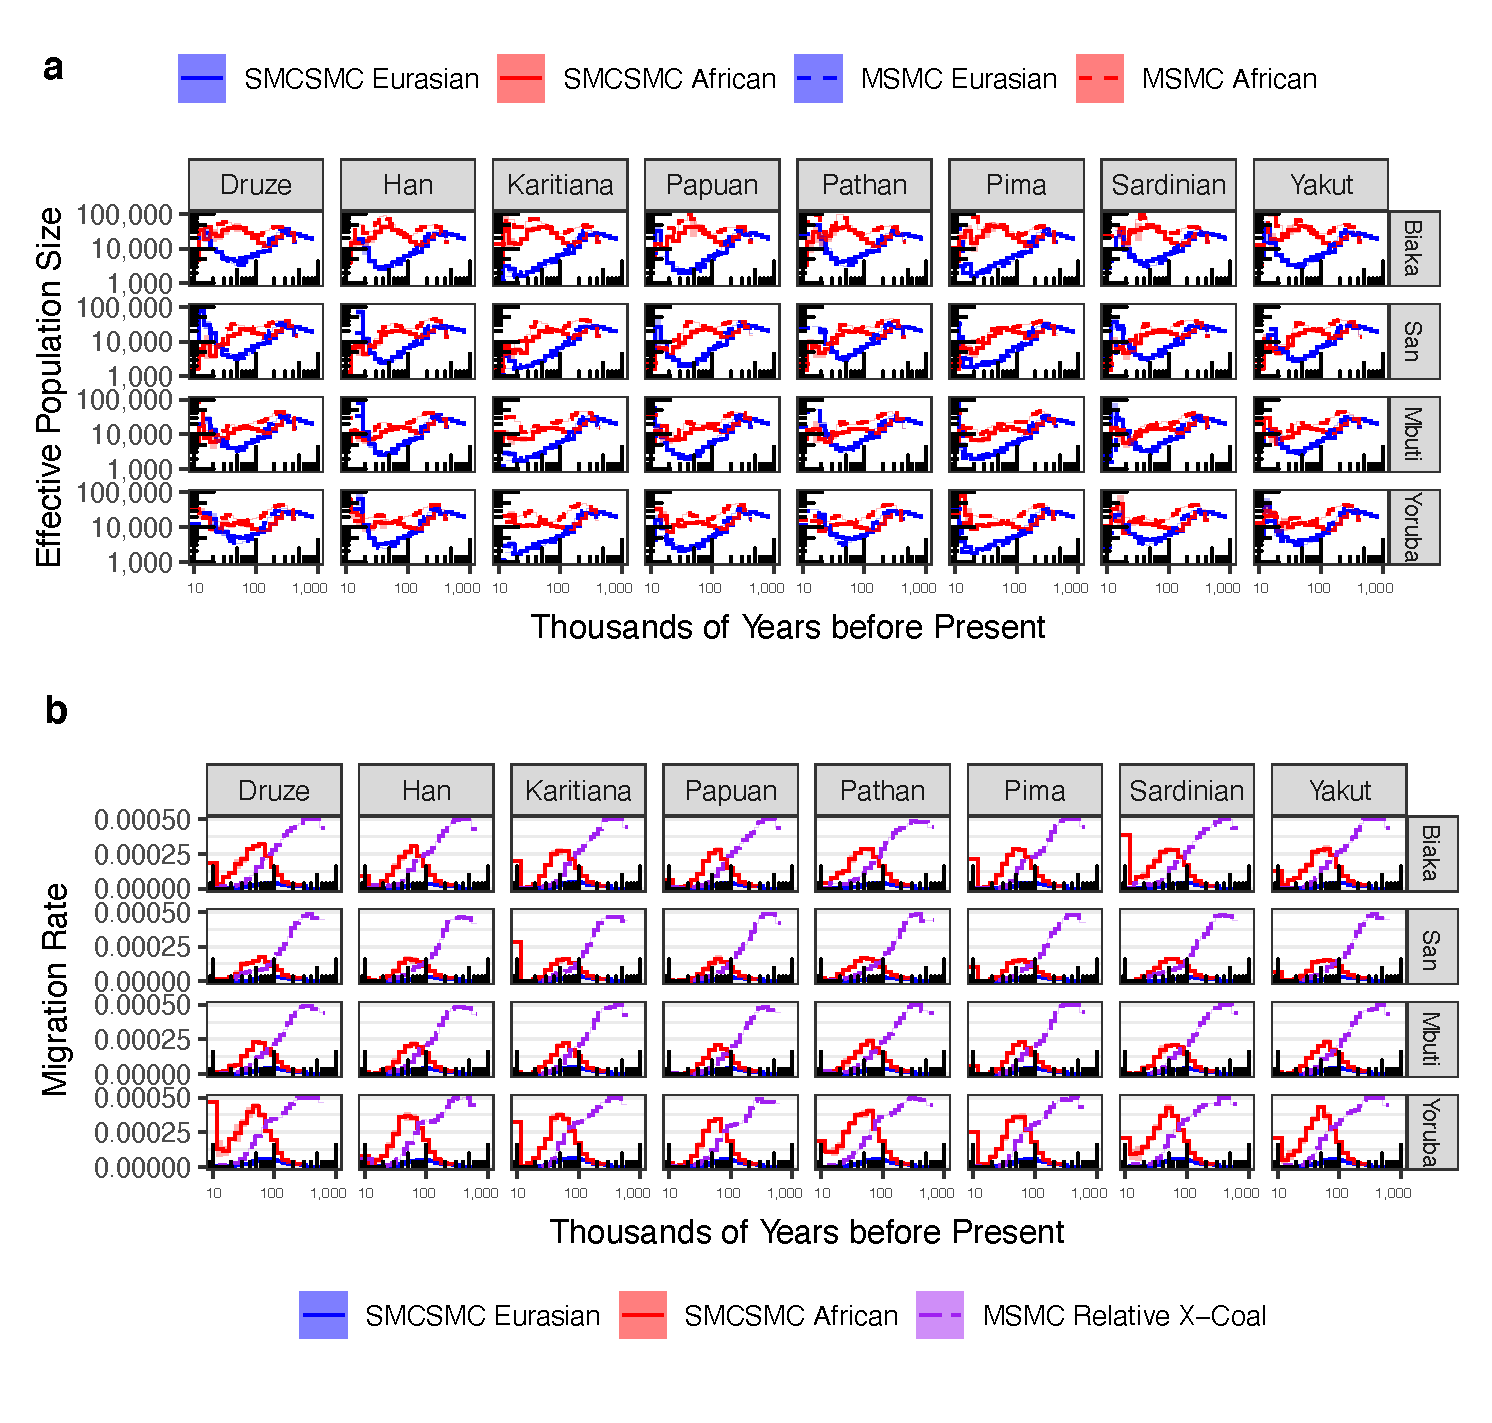
\includegraphics[width=0.9\textwidth]{plot/subset_ne_mig.pdf}
  \caption[Demographic inference in a matched subset of the SGDP]{ Demographic inference in a matched subset of the Simons Genome Diversity Panel. {\bf a.} SMCSMC and MSMC2 inferred effective population size of several populations in the Simons Genome Diversity Panel. These samples were selected to match, as closely as possible, those in the physically phased subset of the Human Genome Diversity Project panel. {b.} Inferred migration using SMCSMC in the Simons Genome Diversity Panel along with the scaled relative cross-coalescent rate estimated by MSMC2.  10,000 particles were used to approximate the ancestral recombination graph in the SMCSMC particle filter and 25 iterations were used to update demographic parameters. 20 iterations were used for MSMC2.}
  \label{fig:hgdp_sgdp}
\end{figure}

\subsection{Simulation demonstrates power to infer large directional migration pulses}

We asked whether SMCSMC has power to detect a large back-migration event in the Late Middle Paleolithic and distinguish it from other demographic scenarios. To answer this we used {\tt SCRM} \cite{Staab2015} to simulate a gigabase of sequence data under a two-island demographic model,
with effective population sizes chosen to be comparable to typical African and Eurasian populations as inferred from real data. 
To this we added a $10$ky pulse of forward, backward or bidirectional migration of varying strengths, with the midpoint of the migration pulse within the range $40$ to $70$kya.  To quantify the inferred amount of migration we calculate the integrated migration fraction (IMF), defined as one minus the probability that a lineage in the destination (e.g.\ African) population traced backwards in time remains in that population across a given epoch according to the migration model (see Methods).  For the simulations, we chose the most recent 100kya as epoch, and used scenarios with IMFs ranging from $0$ to $0.593$. For each simulation we report the inferred IMF in both the forward and backward direction (\Cref{fig:sim}). We find that SMCSMC has good power to detect backward migration pulses up to $60$kya (median ratio of inferred and true IMF, $0.91$), while power drops off at $70$kya (IMF ratio $0.46$). In the pure backward migration case, some forward migration is falsely inferred, but this is always substantially less than the inferred backward migration (median ratio inferred forward to true backward IMF, $0.37$; true migration peak $\leq 60$kya).  However, in the case of true forward migration as well as bidirectional migration, roughly equal mixtures of forward and backward migration are inferred (\Cref{fig:sim}). We conclude that in the epoch $40$--$70$kya the forward and bidirectional scenarios are difficult to distinguish from each other, but both can be distinguished from backward migration, the only scenario resulting in substantially different inferred backward and forward migration.

\begin{figure}
  \centering
  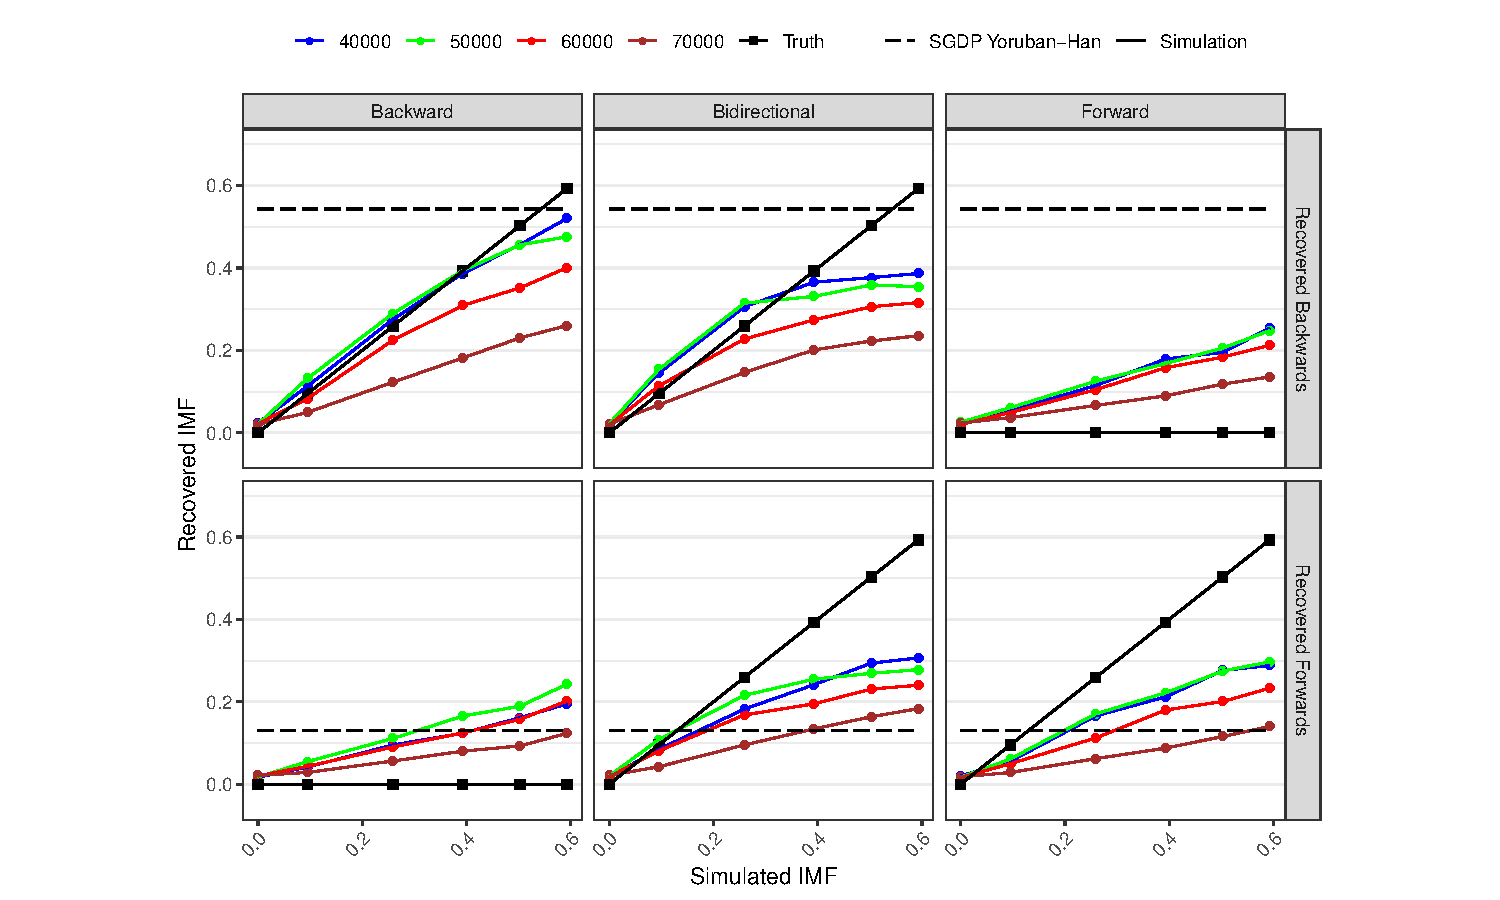
\includegraphics[width=\textwidth]{plot/sim_line_plot.pdf}
  \caption[Simulation Study]{\textbf{Simulation study}. {\tt SCRM} was used to simulate 1 gigabase sequence data for two diploid individuals under three different migration models. Migration was simulated backwards (from a Eurasian-like population to an African-like population), forward (the reverse), and symmetrically (equal migration in both directions). The amount of migration indicates the proportion of the sink population replaced by the source over a 10ky period centered at 40, 50, 60, or 70kya. The total IMF inferred by {\tt SMCSMC} over the last 100ky is plotted and compared to the true simulated amount. For reference, the inferred IMF in either direction across 0-100kya for a Yoruban and Han individual is given in dashed lines.  5 iterations of variational Bayes and 5000 particles were used for inference. The effective population size model and additional details are given in \Cref{methods:simproc}.}
  \label{fig:sim}
\end{figure}


To validate the existence of the migration pulse, though not its direction, we next analyzed the same data using MSMC, which is widely used to estimate gene flow in the ancient past by estimating the relative cross-coalescent rate (RCCR) between two populations \cite{Schiffels2014,Fan2019, Pagani2015, Raghavan2015}. We use the updated implementation MSMC2 recommended by the authors and first published in \cite{Malaspinas2016}. Each of the SMCSMC analyses are repeated using MSMC2 to estimate effective population size and RCCR (\Cref{fig:sgdp_mig}, \Cref{fig:both}, \Cref{fig:sgdp_ne}). Consistent with previous analyses conducted with MSMC2, our estimates show high RCCR in the Late Middle Pleistocene in both the SGDP and the HGDP (\Cref{fig:migrationplot}c,d) \cite{Fan2019, Bergstrom2019}. These observations confirm the existence of a substantial pulse of ancient gene flow between Eurasians (Han Chinese) and Africans.


\begin{figure}
	\centering
	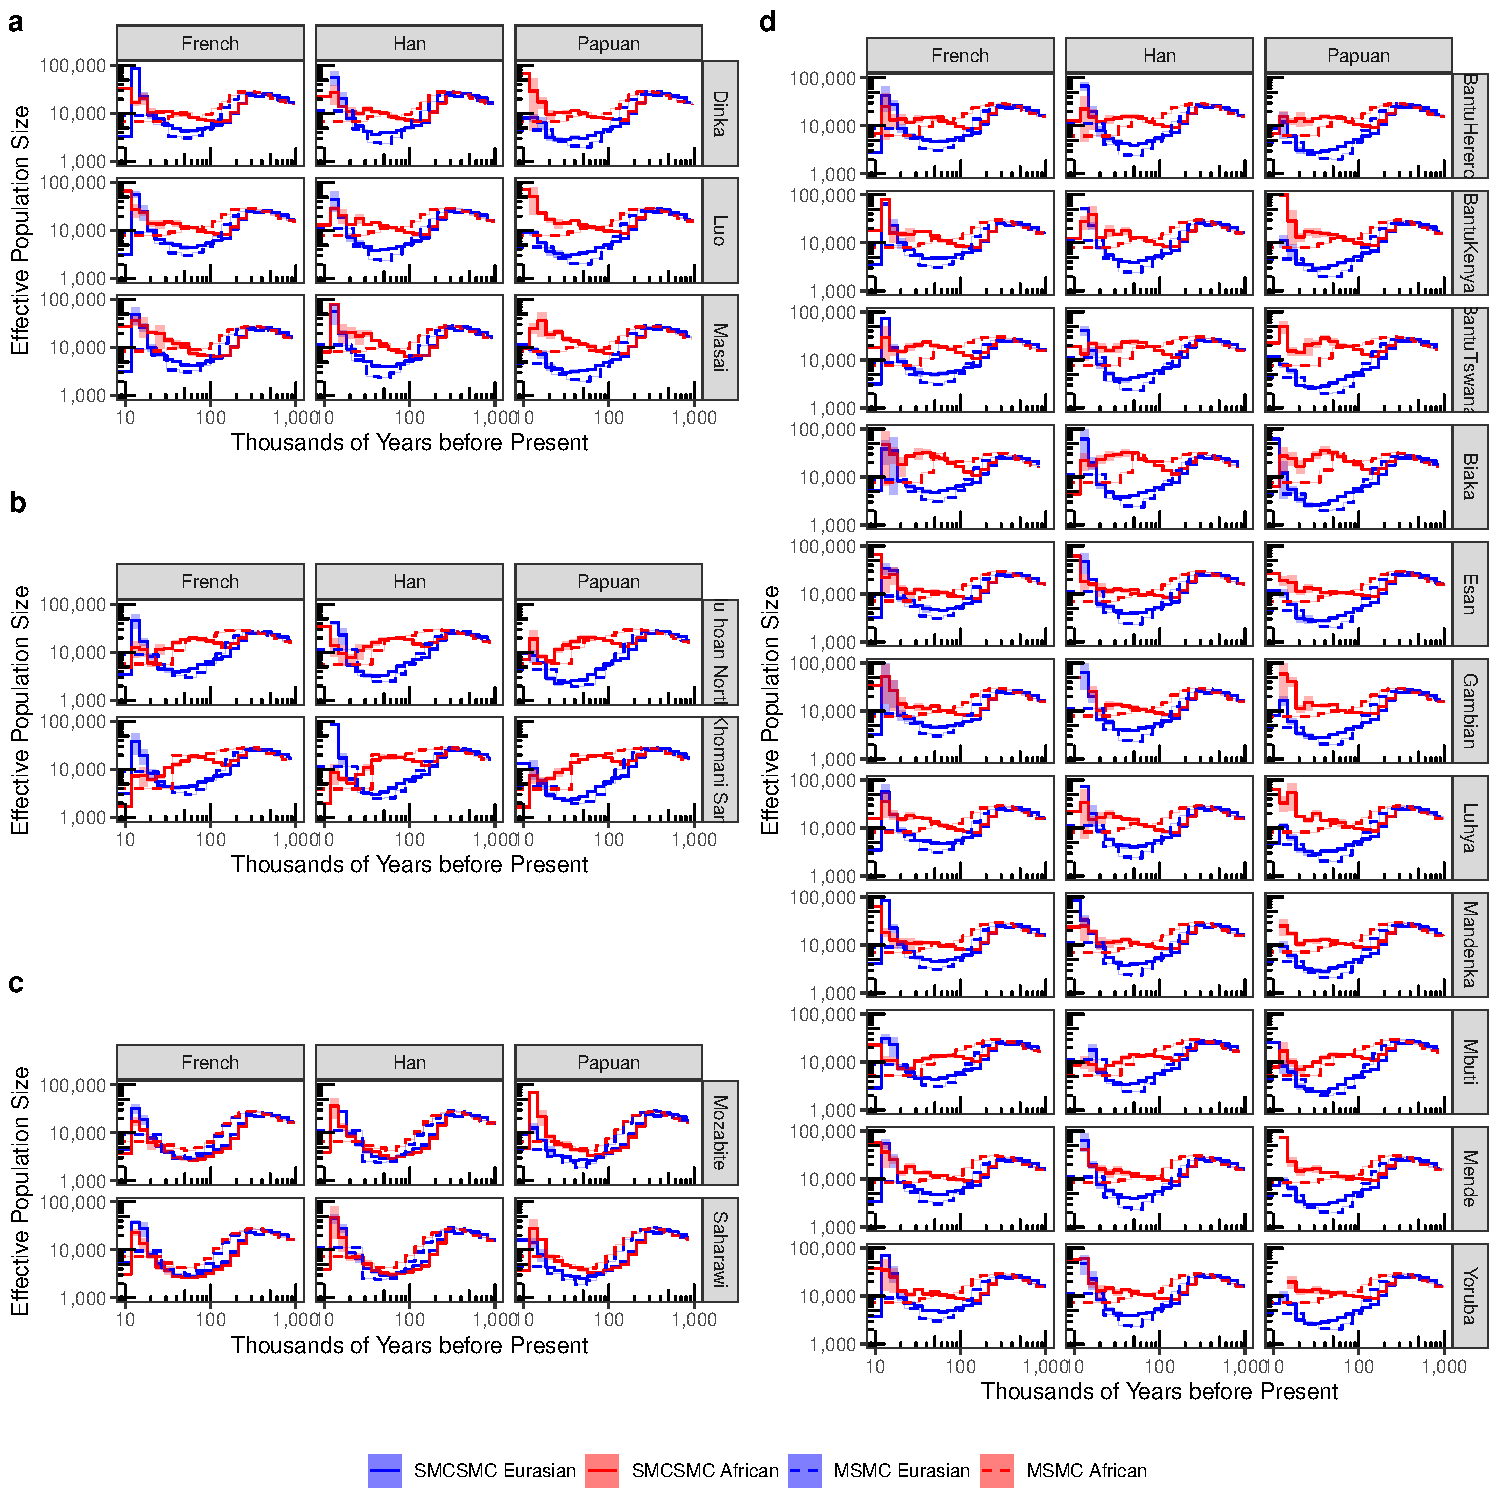
\includegraphics[width=0.95\linewidth]{plot/sgdp_ne_new.pdf}
	\caption[Effective population size inference in the Simons Genome Diversity Project from SMCSMC and MSMC2]{Inference of historical effective population size in the Simons Genome Diversity Project. The SMCSMC particle filter was used to infer directional migration rates and effective population size in both directions from one of three Eurasian populations (French, Han, and Papuan) to one of 18 African populations. 5000 particles were used to approximate the ancestral recombination graph with 10 iterations of variational Bayesian inference to update demographic parameter values. Panels represent a. Nilo-Saharan, b. KhoeSan, c. Afroasiatic, and d. Niger-Kordofanian language families. Alongside the SMCSMC inference, we use MSMC2 to infer the same values with default settings and 20 iterations for convergence.}	
	\label{fig:sgdp_ne}
\end{figure}

\begin{figure}
	\centering
	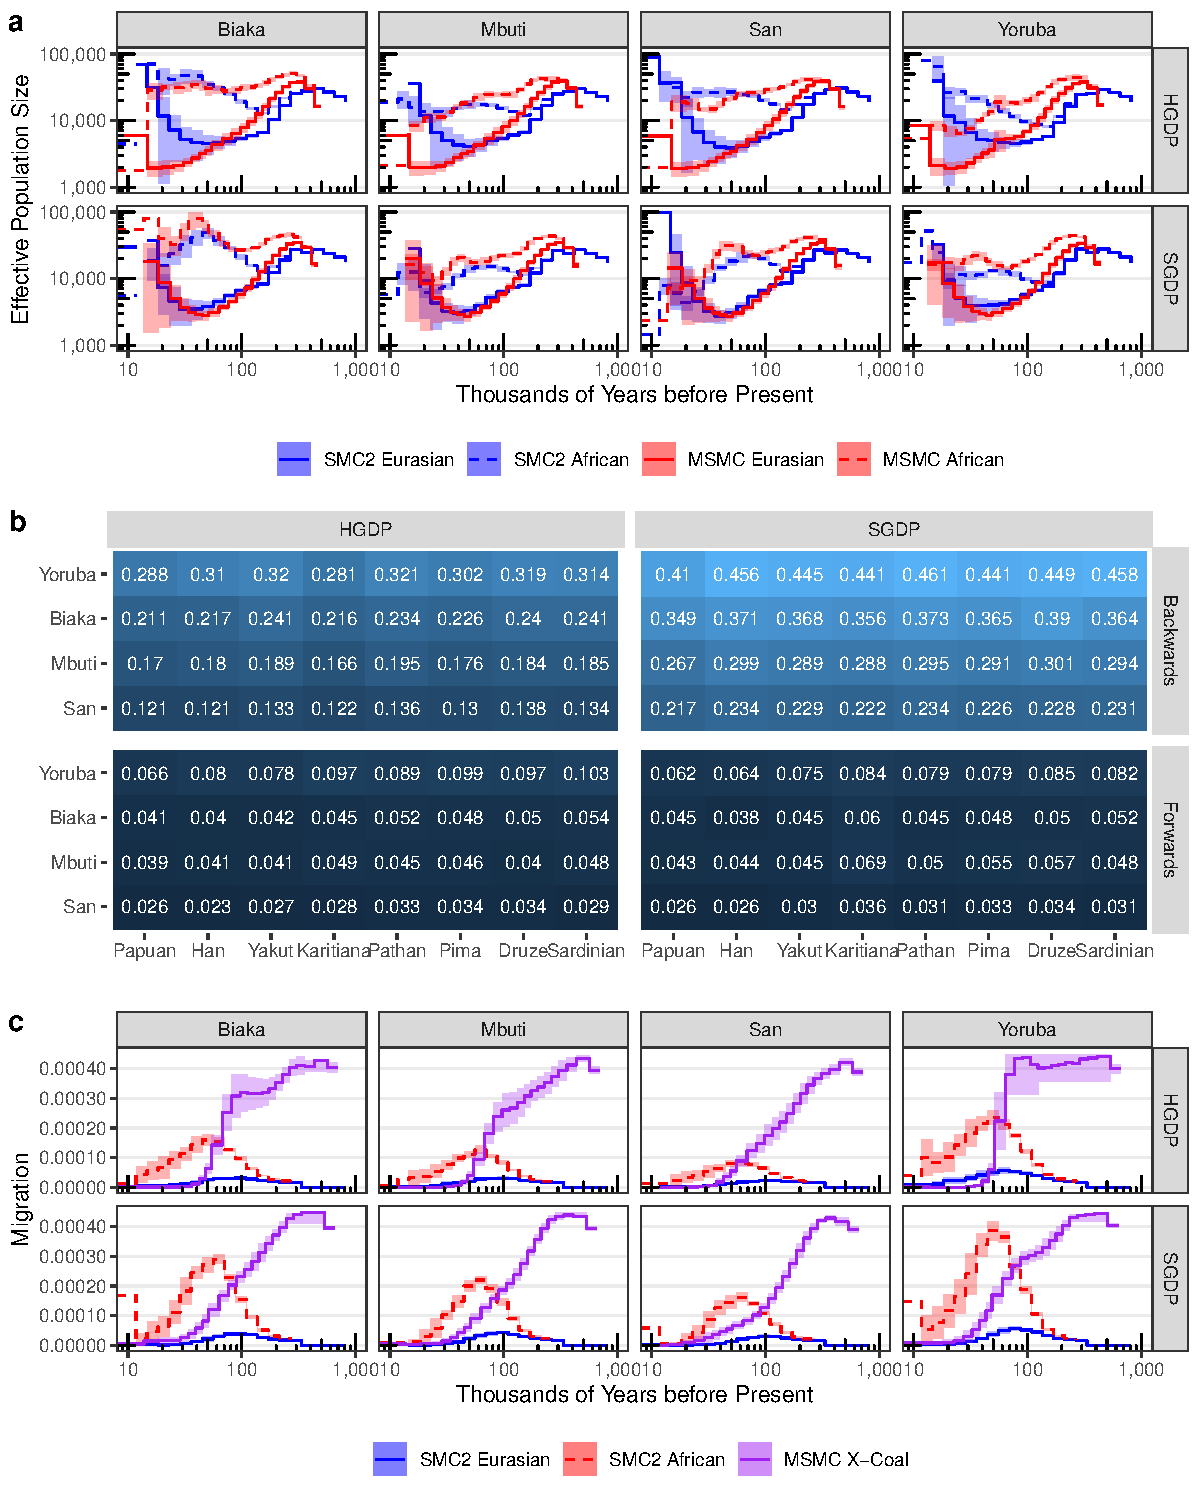
\includegraphics[width=0.7\textwidth]{plot/both_figure.pdf}
	\caption[Migration inference is comparable between phasing strategies]{Inference of directional migration is comparable between data sets and phasing strategies. We used SMCSMC to simultaneously infer directional migration rates and effective population size in the 36 genome physically phased subset of the Human Genome Diversity Panel. We match these 36 genomes with comparable individuals in the Simons Genome Diversity Panel (with the exception of one Papuan population, which has no comparable population in the SGDP) and perform an identical analysis. {\bf a.} Average $N_e$ estimate across four populations in the physically phased subset of the HGDP and the subset of SGDP used to compare with HGDP inference. Inference of population size is averaged over eight Eurasian populations, with the bars representing standard deviation. For MSMC2, the time indexes were averaged to have consistent start and stop times for the steps. {\bf b.} Inferred integrated migration fraction (IMF) from Africa to Eurasians (forwards) and from Eurasians to Africans (backwards) between 40 and 70 kya (see Methods). {\bf c.} Directional migration inference in African populations averaged over Eurasian partners in the two data sets. Shaded regions denote standard deviations. For MSMC, the time indexes were averaged to have consistent start and stop times for plotting.}
	\label{fig:both}
\end{figure}

\subsection{Migration Pre-dates East-West Eurasian Divergence}

To assess whether the inferred back-migration shows variation across the descendants of the OoA event, we repeated the analyses using three representative non-African groups in the SGDP: Han Chinese, French European, and Papuans.  Since simulations show that SMCSMC has little power to detect migration predating 70kya, and to exclude Holocene migration, the epoch we use to calculate real-data IMFs comprise the period of peak inferred migration up to the period of diminishing power (30--70kya); we use this epoch for all subsequent analyses. Inferred IMFs are not significantly different between Han Chinese and European populations in non-Afroasiatic populations (p=0.14, two-tailed paired t-test; \Cref{fig:migrationplot}h and \Cref{fig:sgdp_heatmap}, \Cref{table:average_sgdp_migration_table}), consistent with migration occurring before the European-East Asian split approximately 40kya \cite{Mathieson2014}.  The contribution of this admixture event to extant African genetic variation is substantial; the estimated IMFs indicate that for individuals in the major African language groups, approximately a third of ancestral lineages trace their ancestry through the proto-Eurasian population (Niger-Kordofian group, $0.35\pm 0.04$; Nilo-Saharan groups, $0.41\pm 0.03$; \Cref{table:average_sgdp_migration_table}). When we estimate these proportions using a Papuan sample to represent non-African descendants we find slightly but significantly smaller values compared to estimates using either the Han Chinese or European populations (mean difference of $0.029 \pm 0.002$, p=9.2$\times$10$^{-15}$, and $0.025 \pm 0.004$, p=$2.3\times 10^{-10}$, paired t-tests, \Cref{table:average_sgdp_migration_table}, \Cref{table:sgdp:papuan_imf}). Similarly, in the HGDP, inferred migration in both Papuan groups (Sepik and Highlands) was 0.025 $\pm$ 0.004 (p=$1.4\times10^{-6}$) lower than French and Han (\Cref{table:hgdp:papuan_imf}).  We comment on this observation in the Discussion. 



\begin{figure}
	\centering
	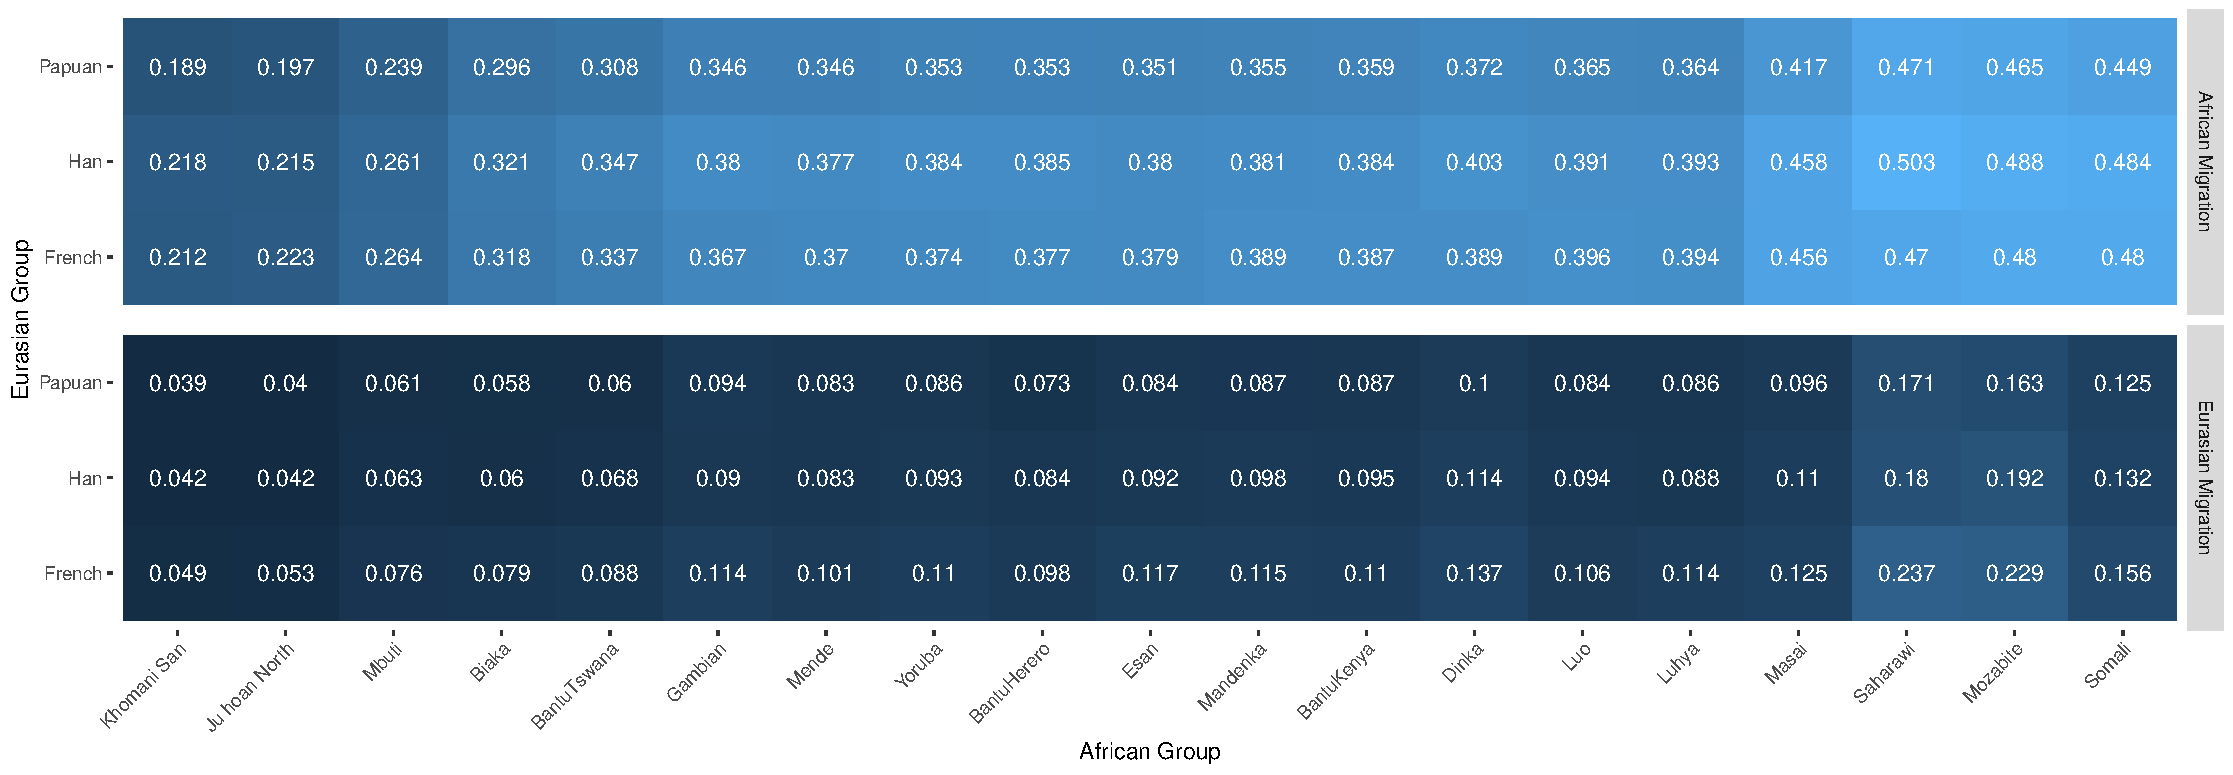
\includegraphics[width=\textwidth]{plot/integrated_sgdp.pdf}
	\caption[Integrated Migration Fraction in the SGDP]{Integrated migration fraction 40--70kya in {\tt SMCSMC} analysed SGDP populations. Directional migration was integrated by finding the cumulative probability of an individual migrating during the specified epoch. Directional migration backwards from Eurasia to Africa and forwards from Africa to Eurasia (both forward in time) are reported separately. Displayed is the average values from three technical replicates.}
	\label{fig:sgdp_heatmap}
\end{figure}

\begin{table}[ht]
  \centering
  \begin{tabular}{rrrrr}
    \hline
   & Estimate & Std. Error & t value & Pr($>$$|$t$|$) \\ 
    \hline
  (Intercept) & 0.3807 & 0.0036 & 105.42 & 1.79e-47 \\ 
    Papuan & -0.0271 & 0.0017 & -15.60 & 7.44e-18 \\ 
    BantuKenya & 0.0051 & 0.0050 & 1.02 & 3.16e-01 \\ 
    BantuTswana & -0.0410 & 0.0050 & -8.13 & 9.49e-10 \\ 
    Biaka & -0.0598 & 0.0050 & -11.87 & 3.53e-14 \\ 
    Dinka & 0.0160 & 0.0050 & 3.17 & 3.05e-03 \\ 
    Esan & -0.0016 & 0.0050 & -0.32 & 7.51e-01 \\ 
    Gambian & -0.0073 & 0.0050 & -1.44 & 1.58e-01 \\ 
    Ju hoan North & -0.1603 & 0.0050 & -31.79 & 1.82e-28 \\ 
    Khomani San & -0.1653 & 0.0050 & -32.80 & 5.96e-29 \\ 
    Luhya & 0.0118 & 0.0050 & 2.34 & 2.46e-02 \\ 
    Luo & 0.0123 & 0.0050 & 2.45 & 1.94e-02 \\ 
    Mandenka & 0.0032 & 0.0050 & 0.63 & 5.34e-01 \\ 
    Masai & 0.0719 & 0.0050 & 14.25 & 1.32e-16 \\ 
    Mbuti & -0.1171 & 0.0050 & -23.22 & 1.17e-23 \\ 
    Mende & -0.0071 & 0.0050 & -1.42 & 1.65e-01 \\ 
    Mozabite & 0.1060 & 0.0050 & 21.02 & 3.63e-22 \\ 
    Saharawi & 0.1097 & 0.0050 & 21.75 & 1.12e-22 \\ 
    Somali & 0.0995 & 0.0050 & 19.73 & 3.12e-21 \\ 
    Yoruba & -0.0013 & 0.0050 & -0.26 & 7.97e-01 \\ 
     \hline
  \end{tabular}
  \slcaption{Linear model predicting integrated migration fraction in the SGDP. The integrated migration fraction (IMF) in the epoch 30--70 kya is obtained as per the Methods section in the Simons Genome Diversity Project.  A binary variable representing Papuan / not Papuan Eurasian donor and categorical variable representing African population were used to predict the IMF in a simple linear model. When adjusted for the different African populations, Papuans contribute less IMF than do other Eurasian partners (French and Han).} 
  \label{table:sgdp:papuan_imf}
  \end{table}
  
  \begin{table}[ht]
  \centering
  \begin{tabular}{rrrrr}
    \hline
   & Estimate & Std. Error & t value & Pr($>$$|$t$|$) \\ 
    \hline
  (Intercept) & 0.3392 & 0.0037 & 92.92 & 1.72e-39 \\ 
    Papuan & -0.0252 & 0.0042 & -5.95 & 1.43e-06 \\ 
    San & -0.1942 & 0.0050 & -38.94 & 6.85e-28 \\ 
    Mbuti & -0.1410 & 0.0050 & -28.27 & 1.07e-23 \\ 
    Biaka & -0.0883 & 0.0050 & -17.69 & 9.33e-18 \\ 
     \hline
  \end{tabular}
  \slcaption{ Linear model predicting integrated migration fraction in the HGDP. The integrated migration fraction (IMF) in the epoch 30--70 kya is obtained as per the Methods section in the physically phased subset of the Human Genome Diversity Project.  A binary variable representing Papuan / not Papuan Eurasian donor and categorical variable representing African population were used to predict the IMF in a simple linear model. When adjusted for the different African populations, Papuans contribute less IMF than do other Eurasian partners (French and Han). } 
  \label{table:hgdp:papuan_imf}
  \end{table}
  

\subsection{Directional Migration Explains Excess Inferred African Genetic Diversity 100kya} 

Previous studies looking at \gls{ne} in human ancestral populations have consistently reported inflated inferences in African populations approximately 100kya, often hypothesized to be due to unaccounted-for population substructure within Africa \cite{Li2011,Schiffels2014}. We use SMCSMC to analyze African individuals paired with an individual from one of three non-African populations (Han Chinese, French European, and Papuans) and infer \gls{ne} for the African ancestral population under a two-island model with directional migration.  Each analysis was repeated three times to assess the contribution of stochastic sampling to the inferences (\Cref{fig:neplot}, \Cref{fig:sgdp_ne}, per population $N_e$ in \Cref{fig:individual_pop_sizes}). SMCSMC infers substantially lower African $N_e$ than MSMC in the period $80$kya--$300$kya.  In addition, while MSMC inferences show convergence of African and Eurasian ancestral $N_e$ estimates only around $300$kya, inferences from SMCSMC indicate convergence at $150$kya (Fig.\ \Cref{fig:neplot}a), closer to the hypothesized time of the diversification of the ancestral lineages prior to the main out-of-Africa migration episode \cite{Timmermann2016, Malaspinas2016}. The same analysis on physically phased samples from HGDP show that these results are not driven by errors due to statistical phasing (\Cref{fig:both} and \Cref{hgdp_section}). When we used SMCSMC to infer both African and European $N_e$ under a single-population model without migration, $N_e$ estimates were comparable to those from MSMC (\Cref{fig:neplot}b), indicating that the SMCSMC inferences are not driven by methodological biases particular to SMCSMC.

\begin{figure}
  \centering
  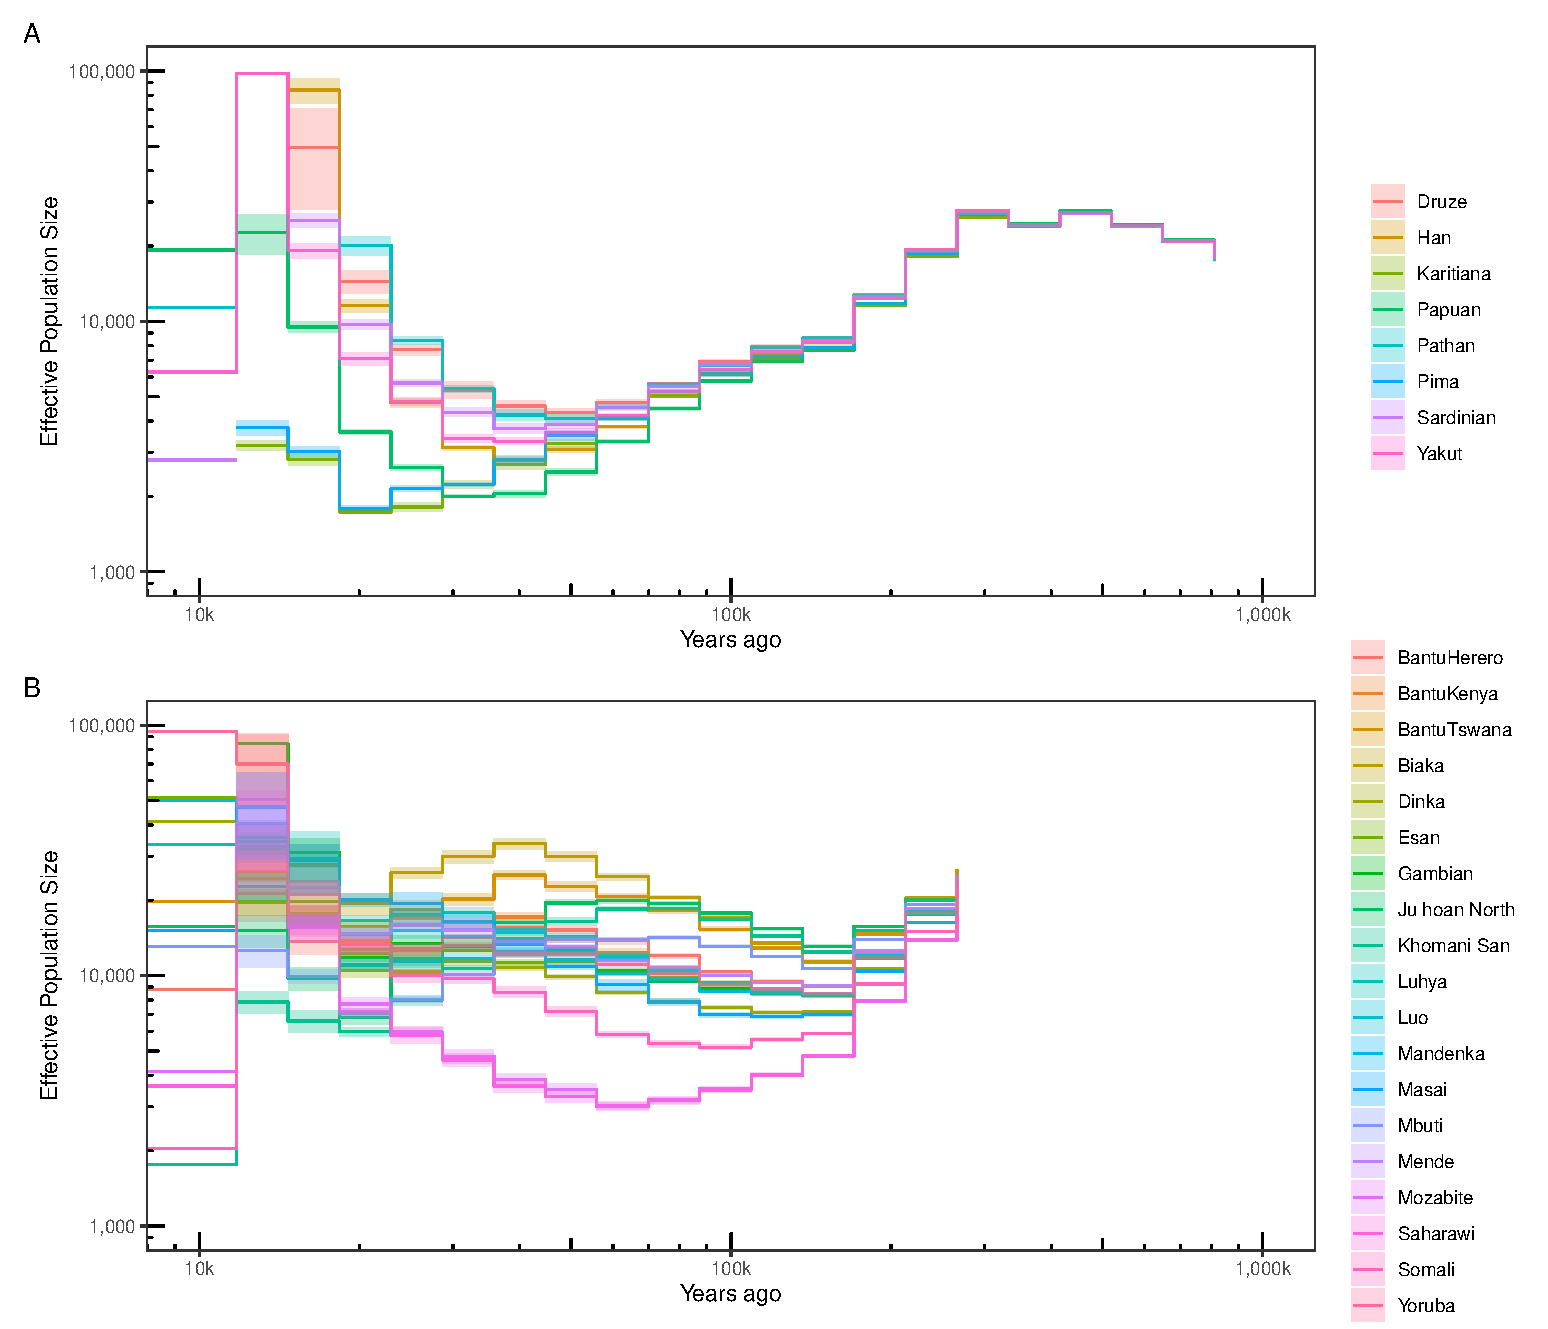
\includegraphics[width=\textwidth]{plot/individual_populations_averaged.pdf}
  \slcaption{\textbf{Estimates of individual population sizes incorporating directional migration.} Using {\tt SMCSMC} the effective population size of global populations in the Simons Genome Diversity Panel is inferred while simultaneously fitting directional migration estimates. Averages are plotted by epoch, with shaded regions denoting the standard deviation. {\bf a.} Estimates of Eurasian population sizes when averaged over Eurasian donor populations. This analysis uses the eight Eurasian populations matched to HGDP populations averaged over the four matched African populations. B. Estimates of African population sizes when averaged over Eurasian recipient populations. This analysis uses the three donor Eurasian populations used for the majority of the analyses in the main text (French, Han, and Papuan) along with the given African populations. Before approximately 250kya, the populations share the same population size within the model, and are not plotted. 10,000 particles are used to approximate the ancestral recombination graph in the SMCSMC particle filter and 15 iterations are used to update demographic parameter values. }
  \label{fig:individual_pop_sizes}
\end{figure}
\newpage


\begin{figure}
	\centering
	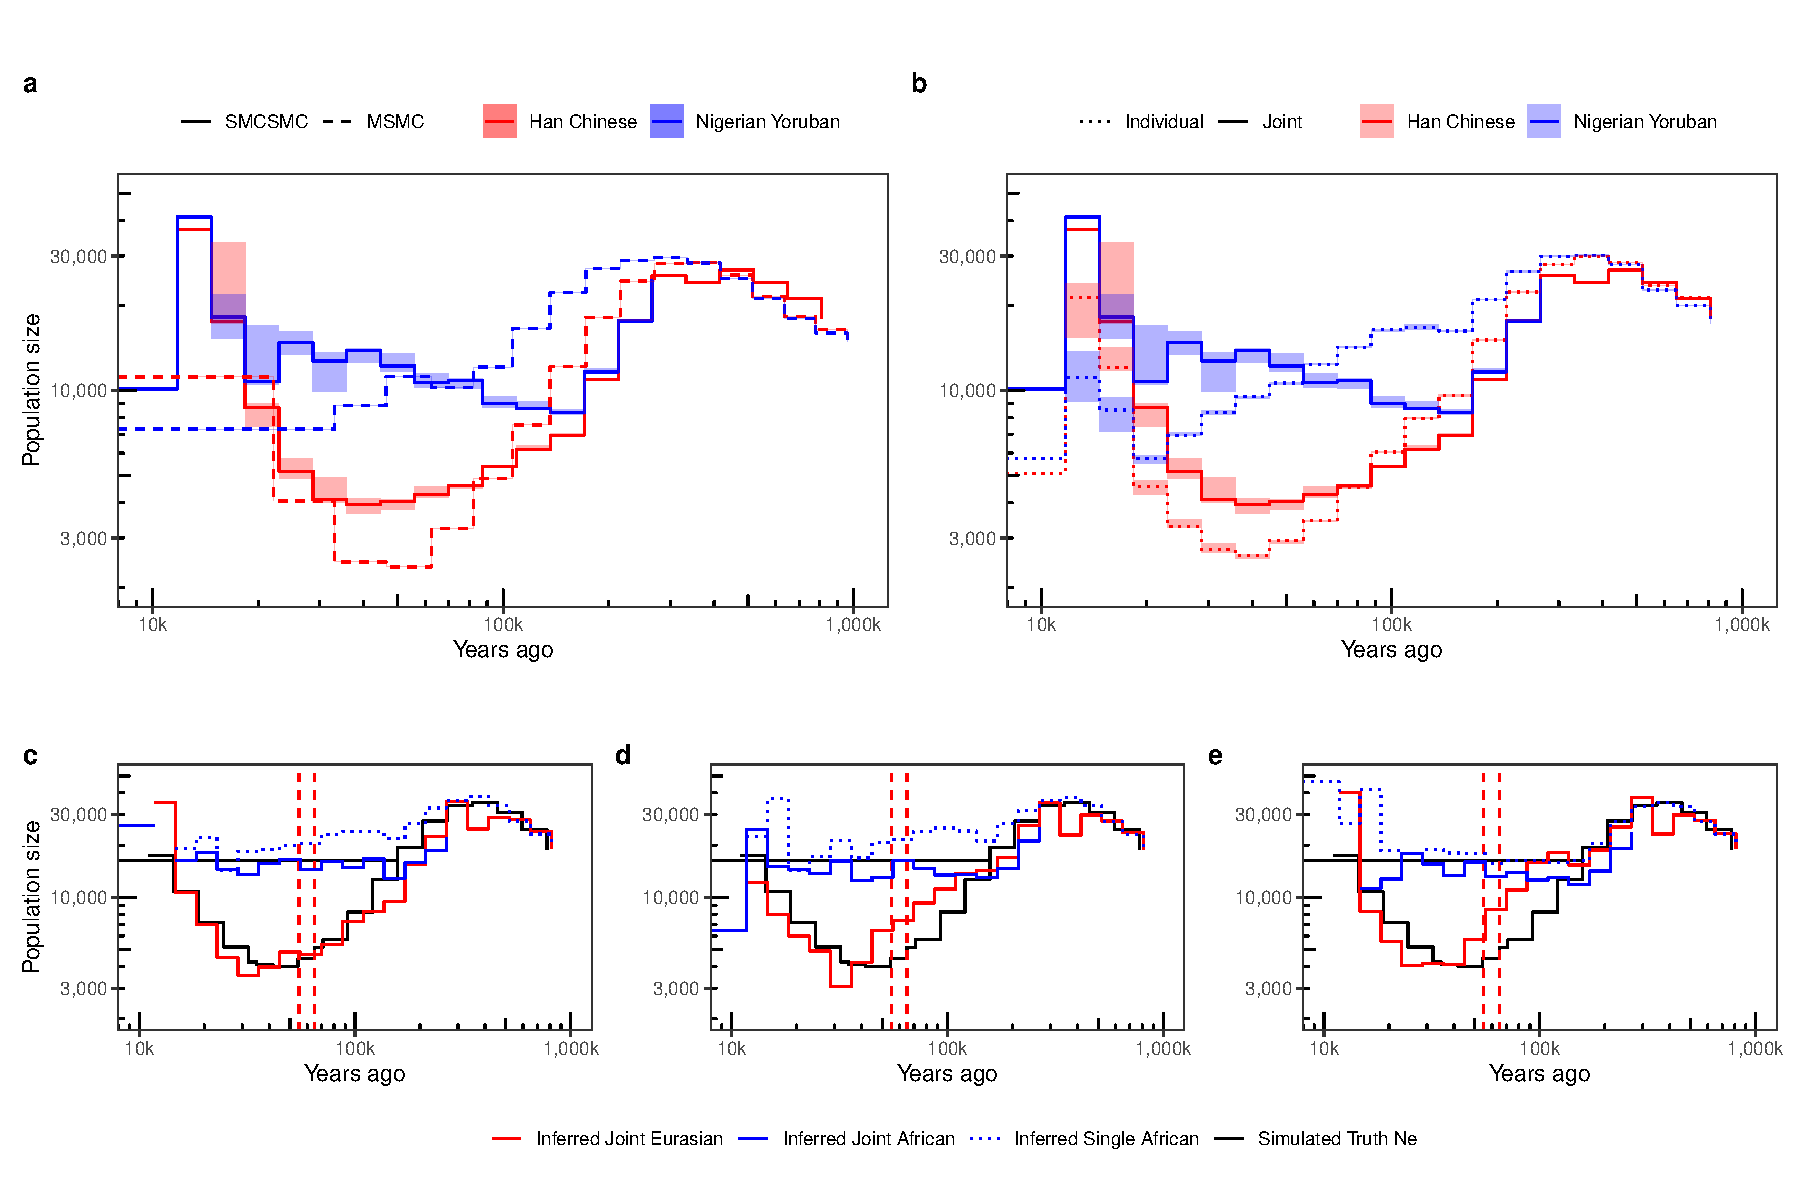
\includegraphics[width=\textwidth]{plot/new_ne_figure.pdf}
	\caption[Effective Population Size Inference]{Effective population size inference. {\bf a.} Analyzing a Nigerian Yoruban and a Han Chinese individual from the Simons Genome Diversity Panel jointly in a two-island model with directional migration using {\tt SMCSMC} yields markedly lower $N_e$ estimates and a more recent apparent split time, than when the same data are analyzed using {\tt MSMC} with a model that does not explicitly include migration. Analyses for {\tt SMCSMC} repeated three times; range of the estimates shaded. {\bf b.} When each individual is analysed separately, using a model not including migration, $N_e$ estimates from {\tt SMCSMC} are similar to those of {\tt MSMC2}. (Joint estimate from {\bf a} included for comparison.) {\bf c, d,} and {\bf e.} 
	Inferred Eurasian and African $N_e$ from data simulated under a two-island model with, from left to right, a backward Eurasia-to-Africa, a bidirectional, and a forward  migration pulse lasting $10$ky (dashed vertical lines; same data as for  \Cref{fig:migrationplot}{\bf e}-{\bf g}).  Particularly for the backward migration case, inferred $N_e$ under a two-island model tracks the true values (black) well, while inferred $N_e$ under a single-population model are inflated around the split time.
 All {\tt SMCSMC} analyses used 10000 particles and 25 variational Bayesian iterations; {\tt MSMC} analyses used 40 iterations (\Cref{methods:simproc}).}
\label{fig:neplot}
\end{figure}

To more directly support the interpretation that the lower African $N_e$ inferred by SMCSMC is due to appropriate modeling of directional migration, we again used coalescent simulation with {\tt SCRM} to investigate various migration scenarios and their effects on inferred African $N_e$. Using the simulation framework as above, we examine $N_e$ estimates inferred under a two-island model with migration, and in addition $N_e$ separately inferred for each of the two simulated populations under a single-population model (\Cref{methods:simproc}).  Focusing on single-population inferences, we found that for simulated African populations that had received substantial migration from the simulated Eurasian population either through backward or bidirectional migration, inferred $N_e$ values indeed were substantially inflated compared to true values (Fig.\ \Cref{fig:neplot}c,d), while this effect was not seen when forward (African-to-Eurasian) migration was simulated (Fig.\ \Cref{fig:neplot}e).  
Similarly, single-population Eurasian $N_e$ estimates were inflated in the presence of forward and bidirectional migration, but not backward migration (\Cref{fig:backsim}--\Cref{fig:fwdsim}).
In contrast, when using a model that includes migration, inferred African $N_e$ do not show inflation in any of the three scenarios (Fig.\ \Cref{fig:neplot}c-e). We conclude that the inferences from SMCSMC and MSMC are compatible with substantial back-migration from ancestral Eurasians into Africans, but not substantial bidirectional or forward migration.

\begin{figure}
	\centering
	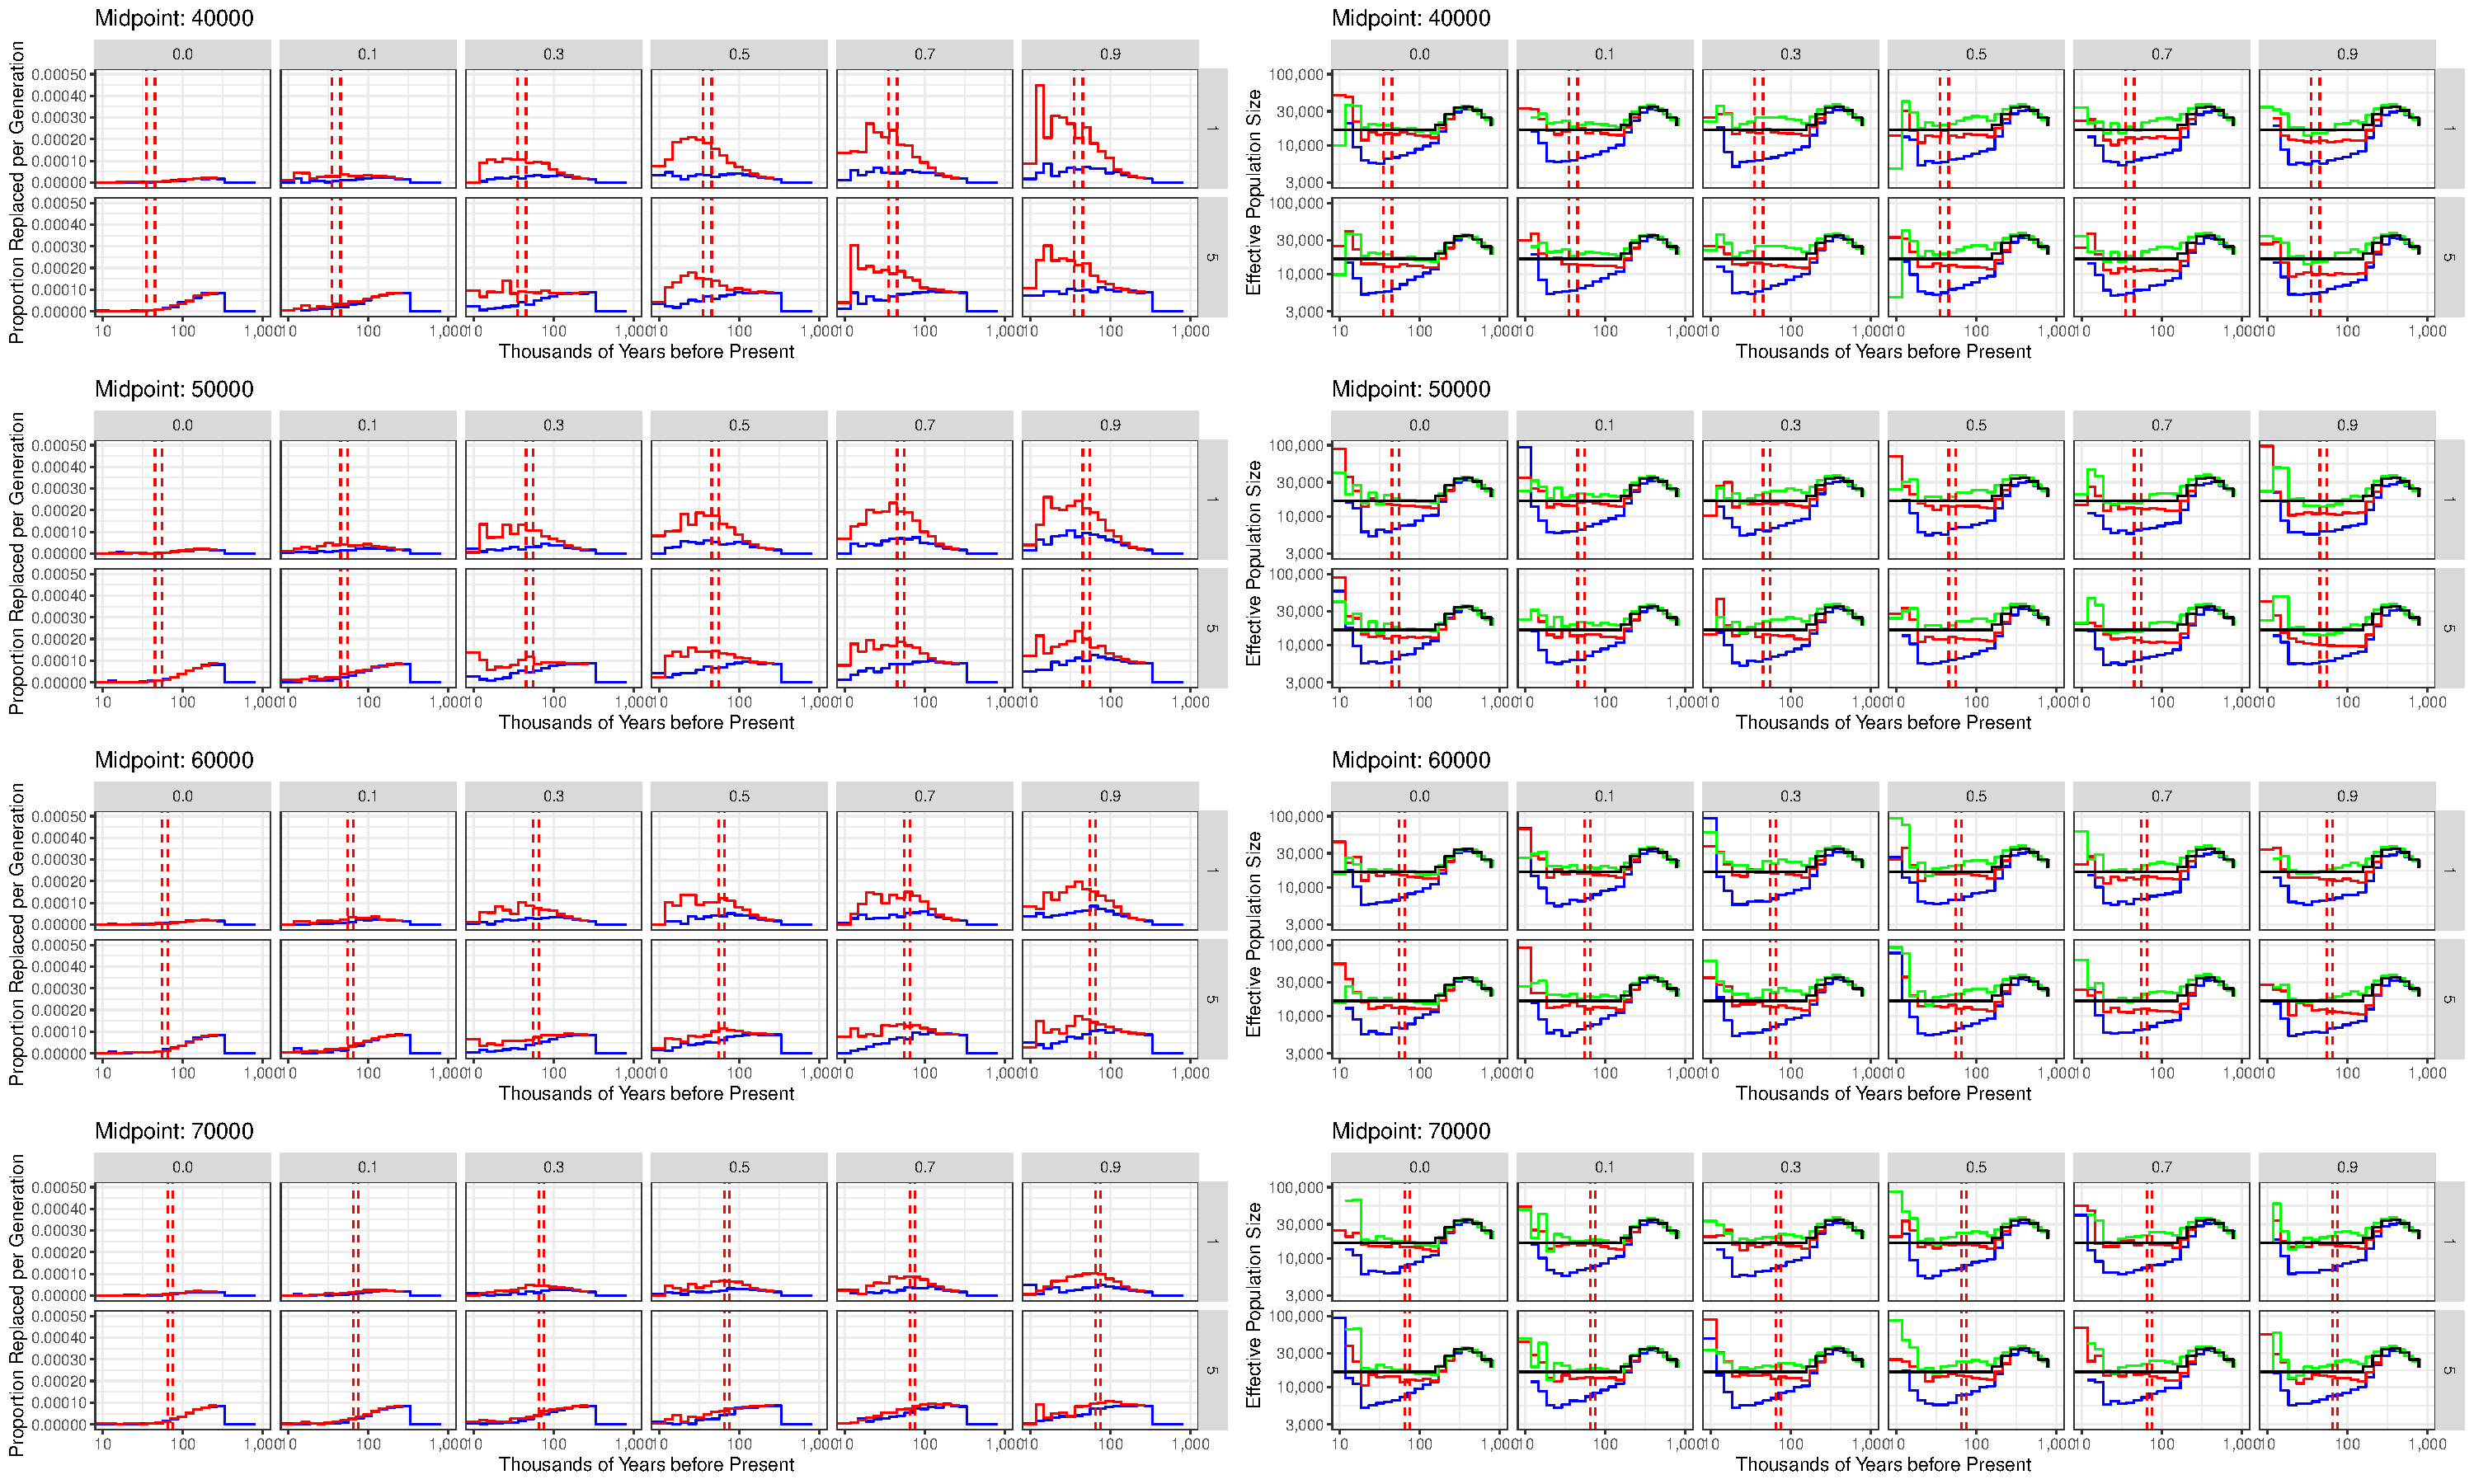
\includegraphics[width=\textwidth]{plot/backward_different_starts.pdf}
	\caption[Simulated migration backwards from effectively Eurasian to effectively African populations]{Simulated migration backwards from effectively Eurasian to effectively African populations. One gigabase of simulated sequence data was generated with {\tt SCRM} for two diploid individuals from different populations using a 100kb sliding window approximation of the coalescent with recombination and a demographic model similar to Eurasians and Africans specified in \Cref{methods:simproc}. The timing, representing the midpoint of a 10ky migration episode, and the integrated migration fraction (IMF) were systematically varied. In this scenario, only backwards migration was simulated. The left panel displays the recovered directional migration, with red lines representing migration backwards from Eurasia and blue representing migration forwards to Eurasia. The timing of the migration episode is demarcated with dotted red lines. The right panel displays the inferred effective population size of both populations. Additionally, the effective population size of the African-like population was modelled separately, without simultaneously inferring migration. 5000 particles were used in the SMCSMC particle filter to approximate the ancestral recombination graph and 5 iterations of variational Bayesian inference were used to updated demographic parameter values.}
	\label{fig:backsim}
\end{figure}

\begin{figure}
	\centering
	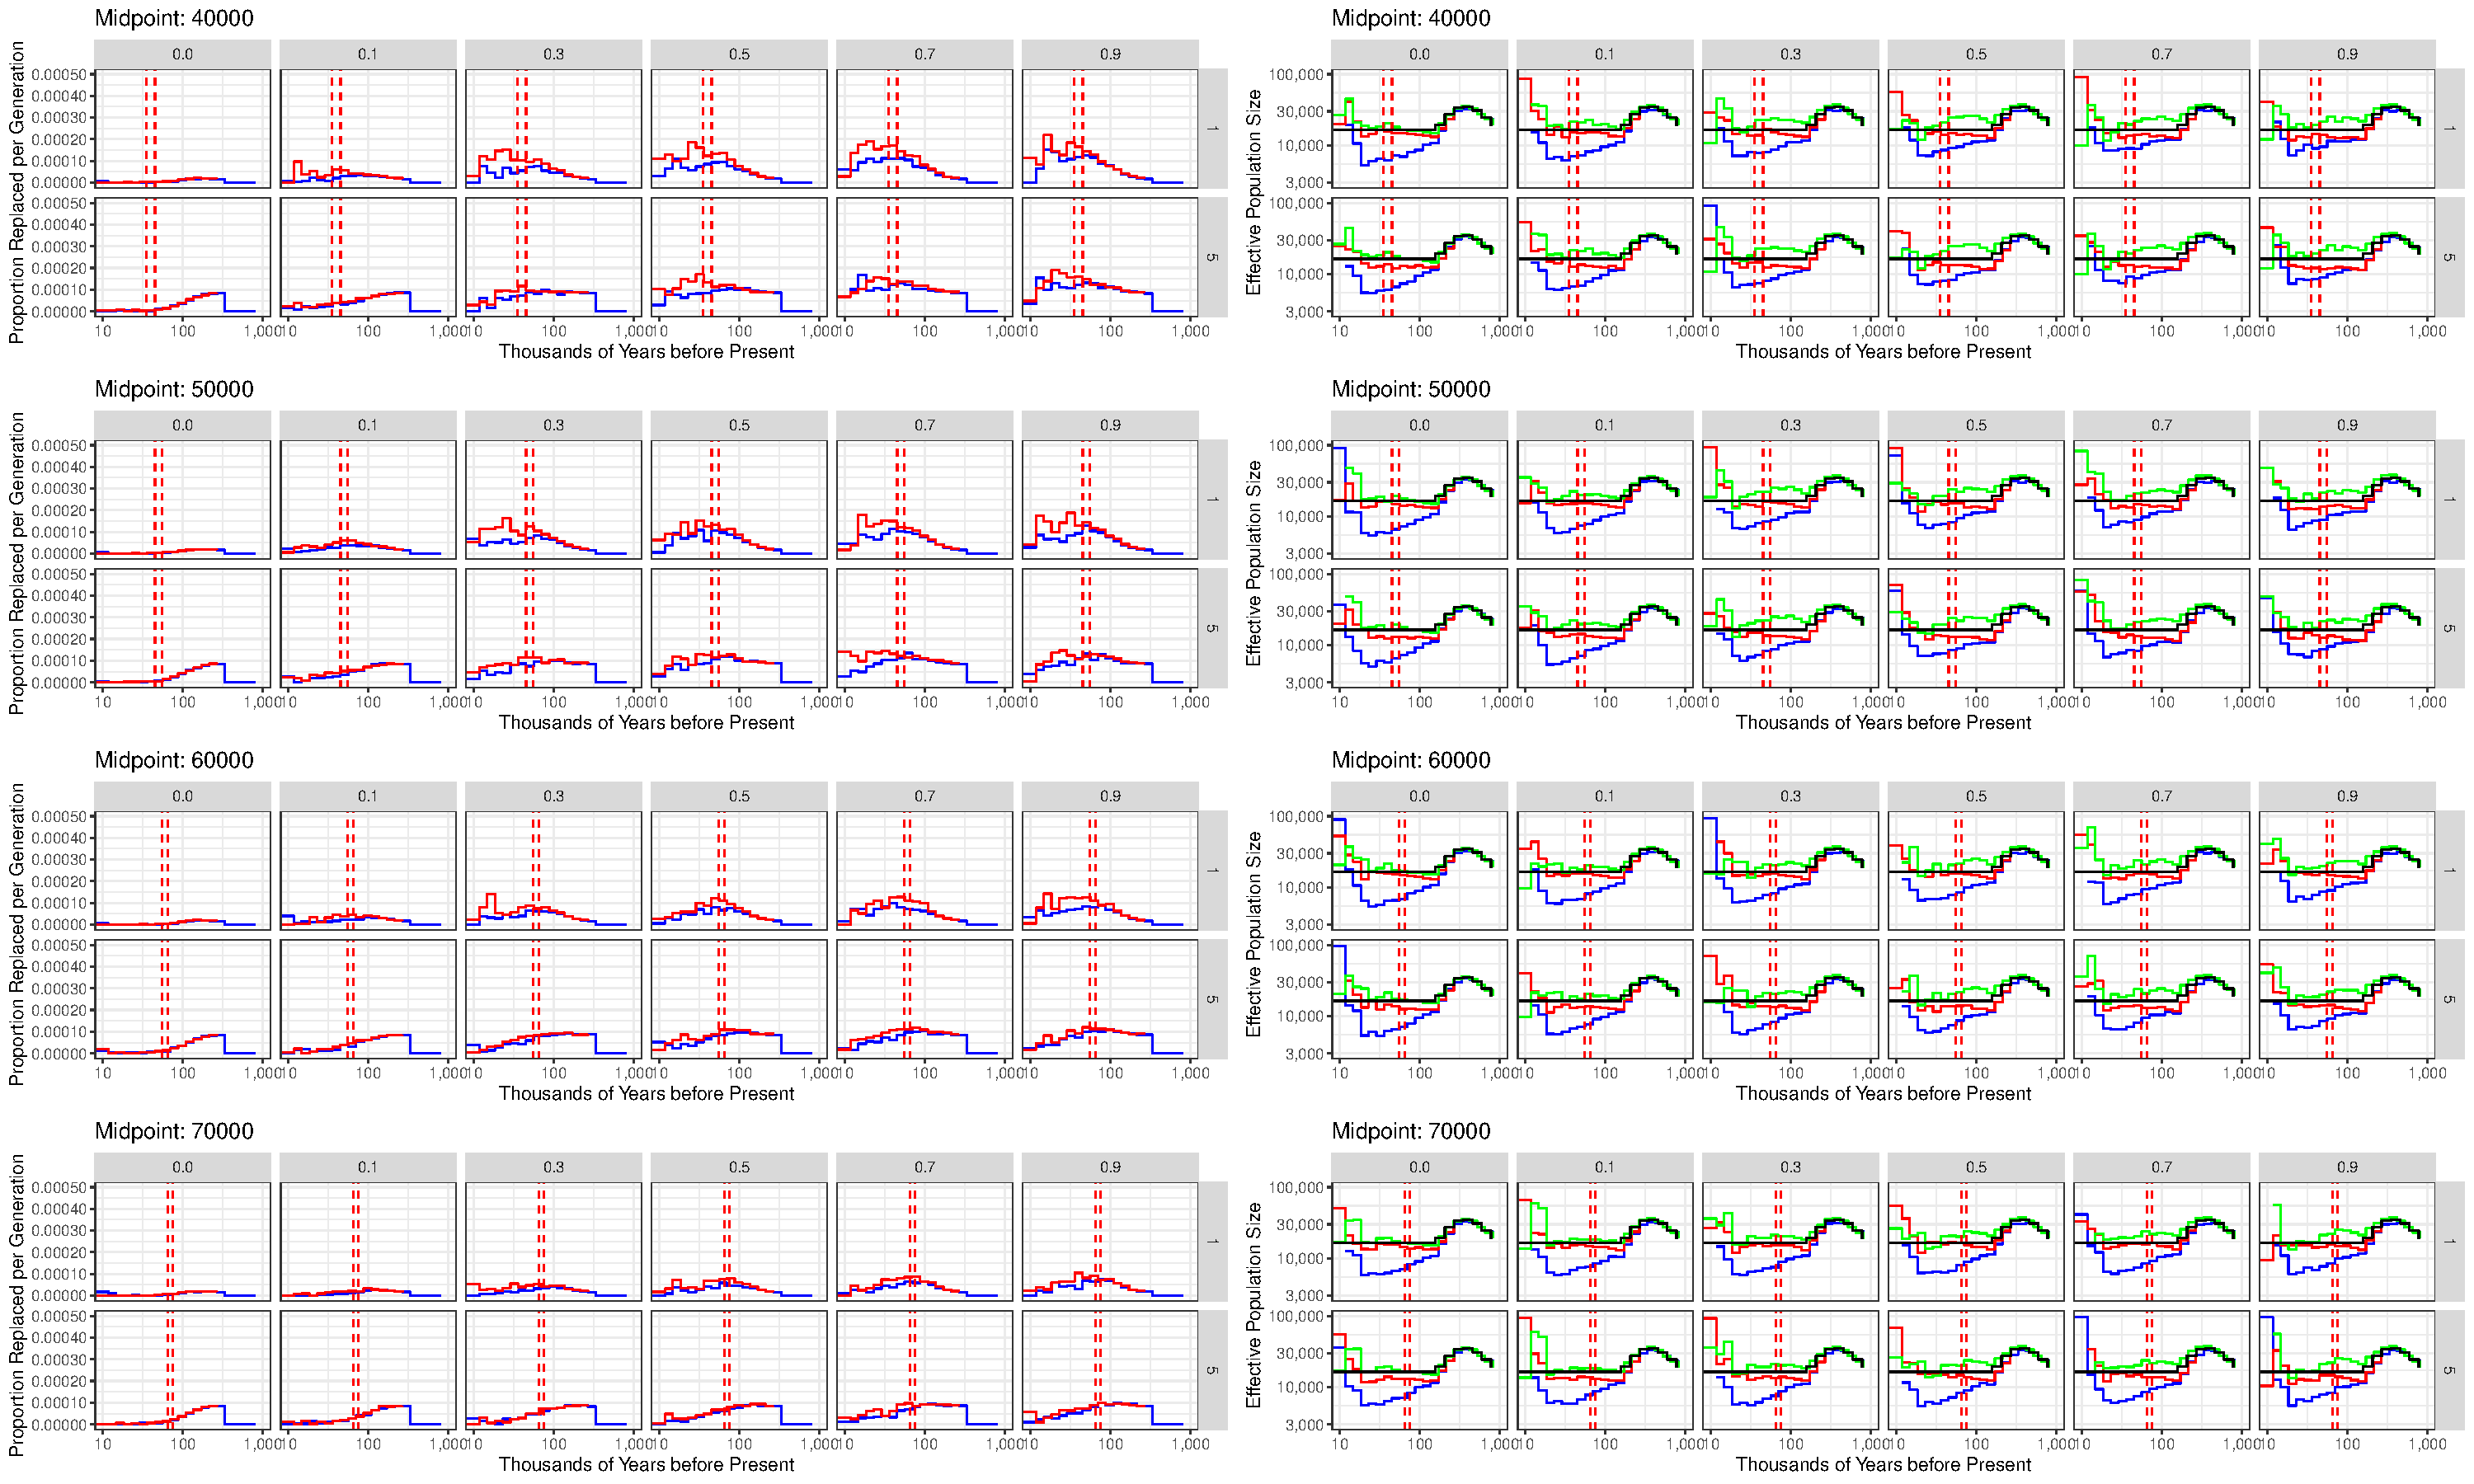
\includegraphics[width=\textwidth]{plot/bidirectional_different_starts.pdf}
	\caption[Simulated bidirectional migration between effectively Eurasian and effectively African populations]{Simulated bidirectional migration between effectively Eurasian and effectively African populations. One gigabase of simulated sequence data was generated with {\tt SCRM} for two diploid individuals from different populations using a 100kb sliding window approximation of the coalescent with recombination and a demographic model similar to Eurasians and Africans specified in \Cref{methods:simproc}. The timing, representing the midpoint of a 10ky migration episode, and the integrated migration fraction (IMF) were systematically varied. In this scenario, migration between these two populations was simulated with equal rates. The left panel displays the recovered directional migration, with red lines representing migration backwards from Eurasia and blue representing migration forwards to Eurasia. The timing of the migration episode is demarcated with dotted red lines. The right panel displays the inferred effective population size of both populations. Additionally, the effective population size of the African-like population was modelled separately, without simultaneously inferring migration. 5000 particles were used in the SMCSMC particle filter to approximate the ancestral recombination graph and 5 iterations of variational Bayesian inference were used to updated demographic parameter values.}
	\label{fig:bisim}
\end{figure}


\begin{figure}
	\centering
	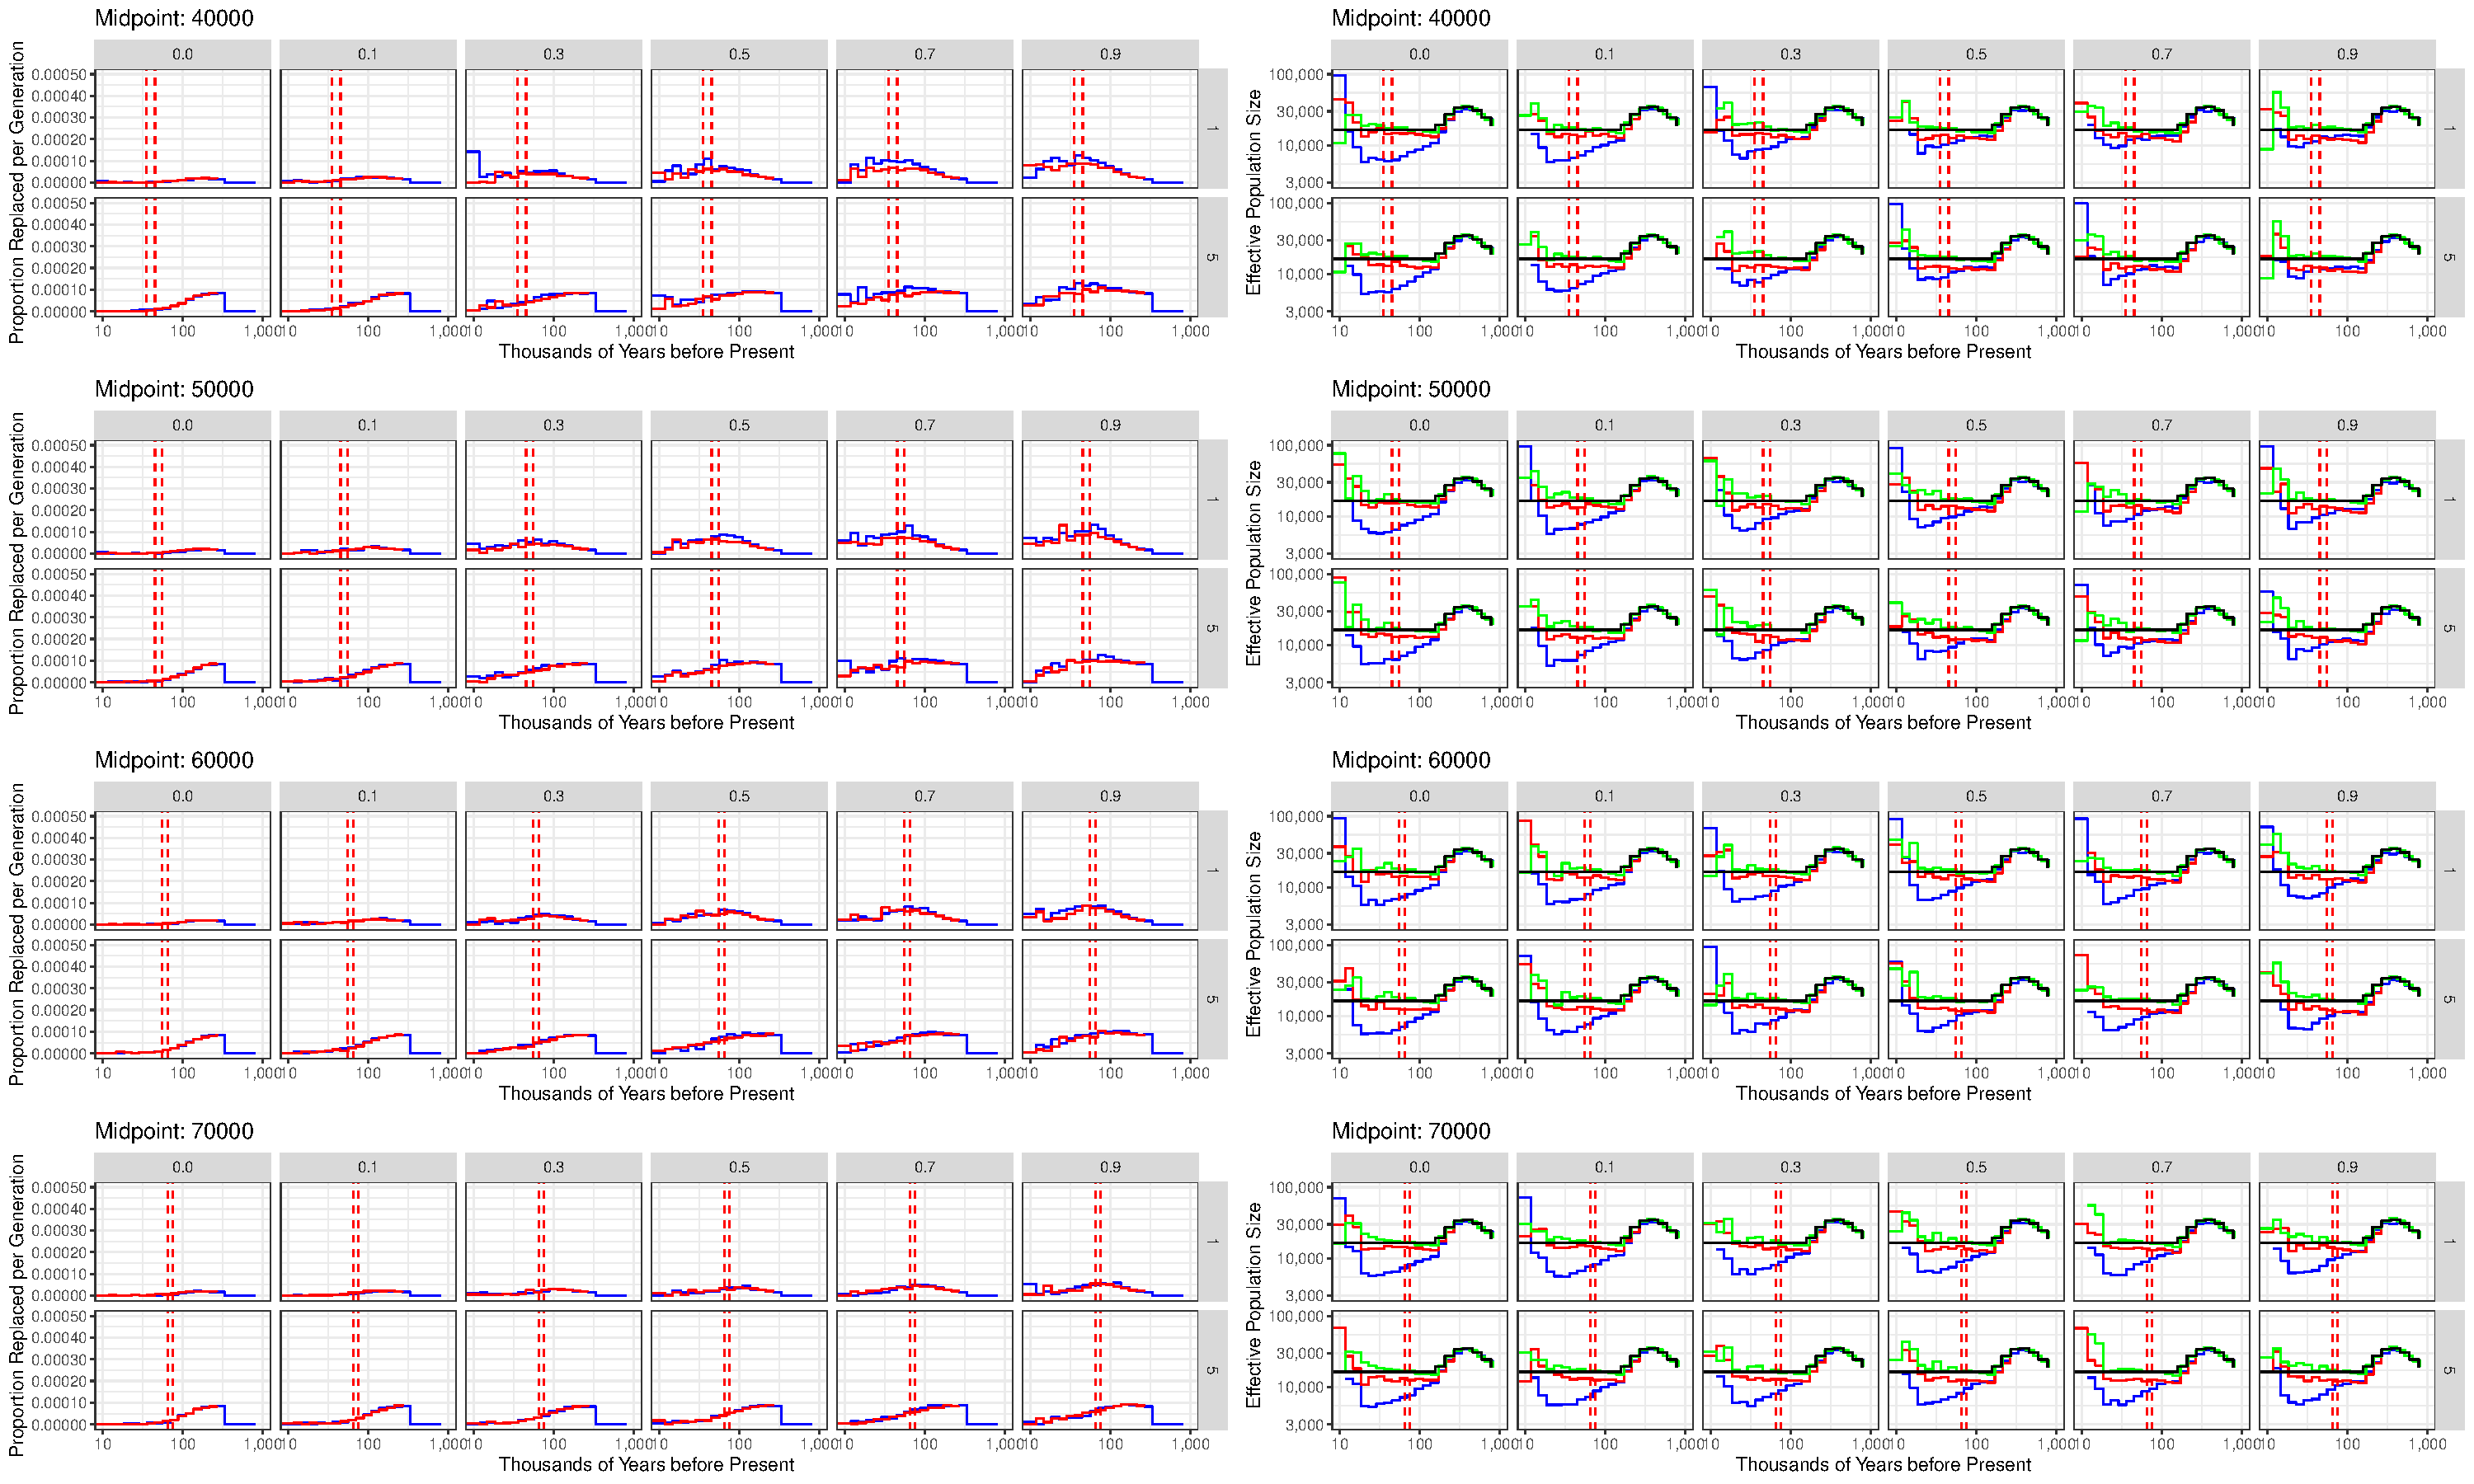
\includegraphics[width=\textwidth]{plot/forward_different_starts.pdf}
	\caption[Simulated migration forwards from effectively African to effectively Eurasian populations]{Simulated migration forwards from effectively African to effectively Eurasian populations. One gigabase of simulated sequence data was generated with {\tt SCRM} for two diploid individuals from different populations using a 100kb sliding window approximation of the coalescent with recombination and a demographic model similar to Eurasians and Africans specified in \Cref{methods:simproc}. The timing, representing the midpoint of a 10ky migration episode, and the integrated migration fraction (IMF) were systematically varied. In this scenario, only forwards migration was simulated. The left panel displays the recovered directional migration, with red lines representing migration backwards from Eurasia and blue representing migration forwards to Eurasia. The timing of the migration episode is demarcated with dotted red lines. The right panel displays the inferred effective population size of both populations. Additionally, the effective population size of the African-like population was modelled separately, without simultaneously inferring migration. 5000 particles were used in the SMCSMC particle filter to approximate the ancestral recombination graph and 5 iterations of variational Bayesian inference were used to updated demographic parameter values.}
	\label{fig:fwdsim}
\end{figure}


\subsection{Less Gene Flow to Central and South African Hunter-Gatherers} We infer substantial Eurasian back-migration into all African groups, however the inferred IMFs for individuals from Khoe-San populations are significantly lower than for any other group (difference with Niger-Kordofians, $0.14 \pm 0.02$, $p = 4.4 \times 10^{-14}$; difference with Nilo-Saharans, $0.20 \pm 0.03$, $p = 6.9 \times 10^{-9}$, two-tailed t-test, \Cref{table:sgdp_pairwise}). To further support this observation we used MSMC to estimate the relative cross-coalescent rate (RCCR) for several populations, and find evidence for gene flow between Yorubans and Eurasians that is not shared with the Khoe-San individuals in either the SGPD and the HGDP (\Cref{fig:migrationplot}c,d). These results are consistent across Eurasian donor populations (\Cref{fig:hgdp_sgdp}). The Khoe-San individuals are particular outliers, whose ancestors are inferred to have experienced approximately half the amount of admixture seen in Nilo-Saharan and Niger-Kordofanian groups (\Cref{fig:sgdp_heatmap}). 
In addition, we find that the Mbuti and Biaka, both Central African hunter-gatherer populations, show levels of Eurasian gene flow that are intermediate between levels observed in the Khoe-San and Yorubans (\Cref{fig:migrationplot}a,b, \Cref{table:average_sgdp_migration_table}).  This is mirrored by inferred IMFs for Central African Hunter Gatherers, which are significantly lower than other Niger-Kordofanian groups (difference $-0.08 \pm 0.03$, $p = 1.2 \times 10^{-3}$, Table \Cref{table:sgdp_pairwise}), possibly reflecting the proposed early split times of the Mbuti and Biaka from the remainder of ancestral African populations between 60 and 200kya \cite{Patin2017, Lipson2019}. 

\subsection{No Evidence for Excess Neanderthal Ancestry} Previous studies have proposed that a backflow from Eurasia may have brought Neanderthal ancestry into African populations \cite{Chen2020}. To assess whether the proposed Late Middle Paleolithic back migration might have introduced Neanderthal material, we analyzed a Yoruban and a French individual using SMCSMC to draw a sample from the posterior distribution of ARGs, isolated the marginal trees containing an inferred back-migration event in the epoch $30$--$70$ \gls{kya}, and reported the inferred admixture tracts. This analysis relies on a sample from the distribution of likely ancestral events, which makes interpreting particular genomic segments challenging. However, along the genome we expect that segments which contain inferred migration events in this period will be enriched for segments truly descended from ancient admixture. Here we study drift within these segments across global populations. 

To assess whether the identified segments are plausible under the demographic model in question, we confirmed that their length distribution is consistent with the IMF and timing of the migration inferred by SMCSMC. We take the isolated segments (\Cref{fig:length}a) and compute the mean track length (\Cref{table:lengths}). We use the approximation that the mean segment length should be approximately equal to $((1-m)r(T-1))^{-1}$ to determine that, if the migration happened in one pulse, our empirical distribution would suggest either a recent timing or a very large pulse (\Cref{fig:length}b). However, we heavily caveat any interpretation of these data with the fact that they are explicitly generated under a model of a given migration proportion. The fact, therefore, that they are of a consistent length with a large migration is more evidence for the model producing internally-consistent tracts than any external validation of the results in this article. 


% latex table generated in R 3.6.2 by xtable 1.8-4 package
% Fri Feb  7 13:46:01 2020
\begin{table}[ht]
  \centering
  \resizebox{\textwidth}{!}{%
  \begin{tabular}{rlrlrlr}
    \hline
  African Population & Mean (SD) & Total (Mb) & Mean (SD) & Total (Mb) & Mean (SD) & Total (Mb) \\ 
    \hline
  Mbuti & 172.204 (189.255) & 939.371 & 165.822 (182.549) & 850.335 & 163.352 (181.607) & 756.320 \\ 
    Biaka & 172.332 (184.183) & 1057.083 & 169.296 (185.457) & 1052.004 & 170.149 (185.853) & 1044.036 \\ 
    Khomani San & 173.06 (188.492) & 671.125 & 169.005 (183.871) & 706.777 & 166.33 (175.899) & 597.125 \\ 
    Ju hoan North & 175.415 (195.979) & 747.618 & 171.909 (187.835) & 711.186 & 161.146 (175.476) & 656.024 \\ 
    Luhya & 177.303 (193.164) & 1370.729 & 181.025 (197.94) & 1403.123 & 175.821 (192.259) & 1211.762 \\ 
    Esan & 177.483 (191.148) & 1364.132 & 178.429 (190.819) & 1426.180 & 170.451 (183.886) & 1270.204 \\ 
    Gambian & 177.804 (195.646) & 1333.529 & 177.099 (191.542) & 1304.155 & 173.892 (185.544) & 1213.071 \\ 
    Luo & 178.653 (192.447) & 1368.481 & 175.618 (192.833) & 1361.917 & 180.635 (201.159) & 1348.798 \\ 
    BantuHerero & 179.691 (194.451) & 1354.869 & 176.473 (188.855) & 1327.779 & 178.544 (198.496) & 1310.511 \\ 
    BantuTswana & 180.309 (195.176) & 1150.551 & 174.826 (188.153) & 1159.796 & 172.542 (192.6) & 1096.674 \\ 
    Mende & 182.087 (200.591) & 1256.580 & 177.24 (197.23) & 1288.533 & 169.901 (182.944) & 1191.515 \\ 
    Yoruba & 184.255 (199.949) & 1283.151 & 176.276 (193.69) & 1361.031 & 169.867 (181.948) & 1275.701 \\ 
    BantuKenya & 184.419 (200.395) & 1265.297 & 173.485 (191.175) & 1269.739 & 179.415 (189.784) & 1214.104 \\ 
    Mandenka & 185.35 (206.972) & 1411.440 & 176.908 (194.337) & 1328.754 & 172.03 (182.984) & 1265.625 \\ 
    Masai & 186.769 (209.675) & 1353.890 & 182.366 (198.06) & 1483.361 & 181.22 (199.255) & 1438.160 \\ 
    Mozabite & 194.378 (214.029) & 1318.273 & 193.469 (211.945) & 1557.040 & 188.867 (210.994) & 1532.842 \\ 
    Saharawi & 197.668 (218.662) & 1383.280 & 196.156 (217.233) & 1406.245 & 195.045 (217.263) & 1585.907 \\ 
     \hline
  \end{tabular}}
  \slcaption{Summary of the length distribution for putatively migrated segments in different African individuals. Means and standard deviations are given in kilobases (kb) while the total length of all segments is given in megabases (Mb).} 
  \label{table:lengths}
  \end{table}
  


\begin{figure}
  \centering
  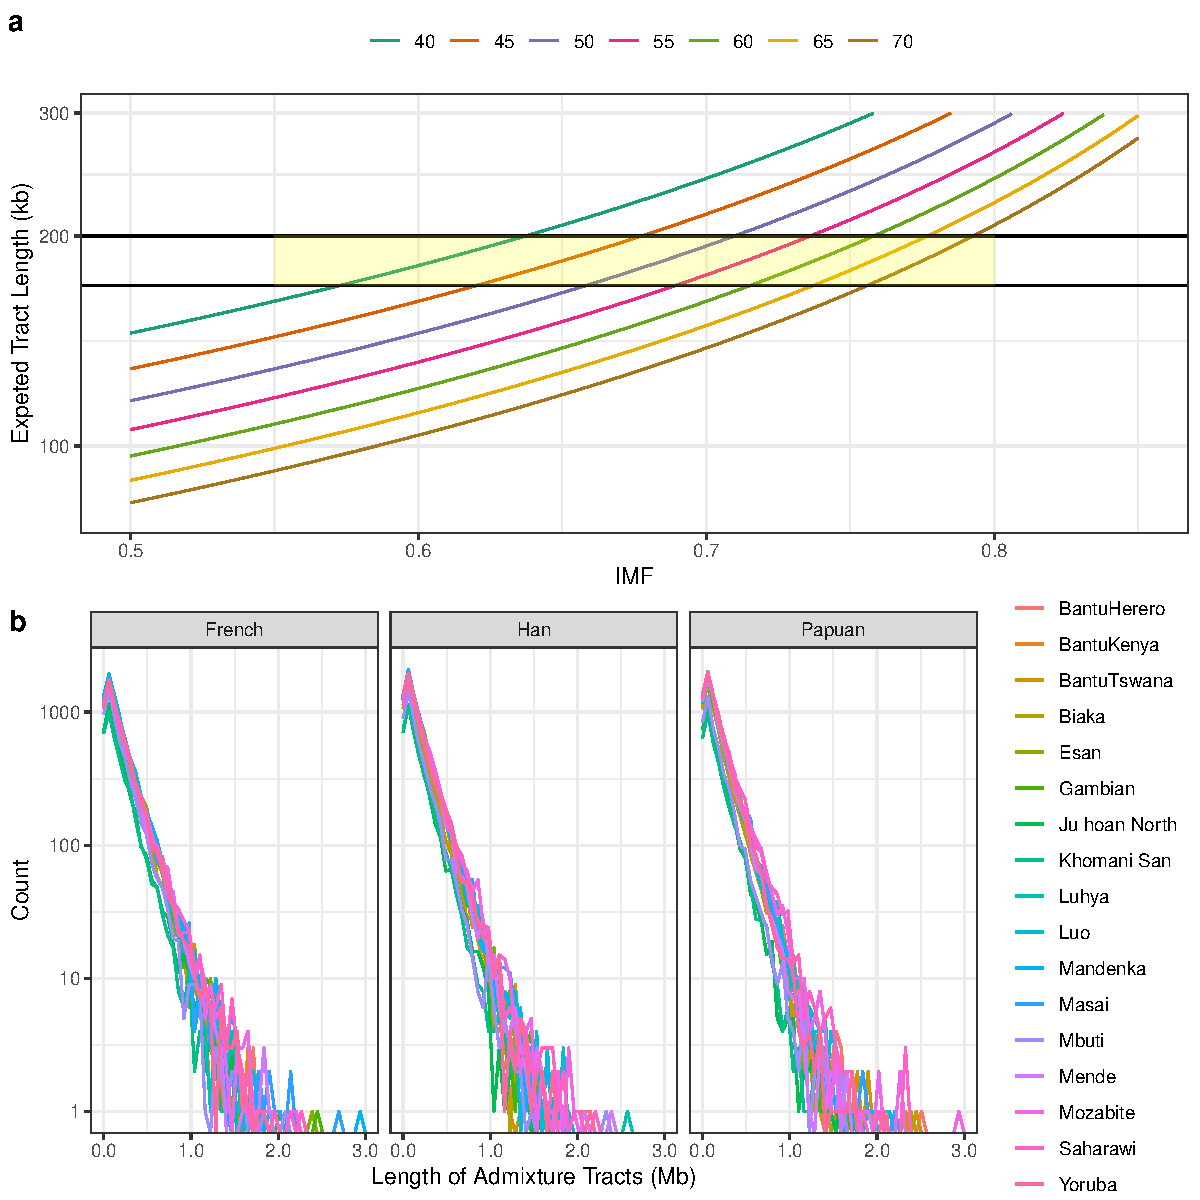
\includegraphics[width=\textwidth]{plot/both_length.pdf}
  \slcaption{Analysis of the length of putatively migrated segments. {\bf a.} Theoretical length distribution of admixture tract rate parameter under varying migration and admixture timing assuming that $L = ((1-m)r(T-1))^-1$, given $L$ length, $m$ symmetrical migration rate, $r$ recombination rate in events per nucleotide, and $T$ time in generations \cite{Liang953}. Shaded region denotes empirical range (with San at the bottom end, and Yoruban at the top end, \Cref{table:lengths}) of fragments observed in the Simons Genome Diversity Panel. {\bf b.} Following the reconstruction of the ancestral recombination graph using different African and non-African individuals using the {\tt SMCSMC} particle filter, we use a sample of the posterior distribution of marginal trees to reconstruct putatively migrated segments (see Methods). We plot the length distribution of admixture tracts between individuals in the SGDP using 50 bins. Length is given in megabases (Mb). Isolated from {\tt SMCSMC} estimated ancestral recombination graphs. Migration rate is given in terms of proportion of the sink population replaced per generation. }
  \label{fig:length}
\end{figure}


The assumption that migration has occurred in a single wave is largely unrealistic. We used expectation maximization to investigate if a mixture of exponential distributions explained the observed tract lengths better than a single distribution. We found that in some cases, two or three exponential distributions were better supposed by the data, however the differences in log likelihoods was negligible and the support for the different distributions was approximately inversely proportional to their number (data not shown). We found no strong support for multiple waves of migration from this analysis.


As expected, we found that these African segments with putative Eurasian ancestry tend to be more closely related to a Eurasian sample than another representative of the same African population (\Cref{dstats:a1}, \Cref{fig:f3}, \Cref{fig:f3_admix}) in a global dataset of modern and ancient individuals compiled by the Reich group (see URLs). Within these African segments that are likely enriched for material with Eurasian ancestry, we then used $D$ statistics \cite{Patterson2012} to identify enrichment for Neanderthal material compared to an African background. 

We first use $f_3$ statistics to look for evidence of admixture between the African and various Eurasian groups. Thus, we calculate $f_3$(Yoruba-1, Eurasian group, Yoruba-2) for Papuans, French, Han Chinese, and the Vindija Neanderthal. We calculate this statistic in all available markers, and additionally for the segments isolated from the three Eurasians separately (\Cref{fig:f3}). These statistics show, firstly, that ascertaining in a particular group influences the shared drift with that group. This is exemplified by the non-significant shared drift with Papuans in French and Han ascertained segments. Secondly, these statistic show significant levels ($|Z|>2$) of drift between the test individual and Eurasian populations, while also showing no increase in Neanderthal allele sharing ($f_3$ = 0). To find statistical evidence of admixture, we compute $f_3$(Yoruba-2, Eurasian, Yoruba-1) for the same Eurasian groups. We find statistical evidence for admixture in each of the groups examined, for all ascertainment schemes (\Cref{fig:f3_admix}). 


\begin{figure}
  \centering
  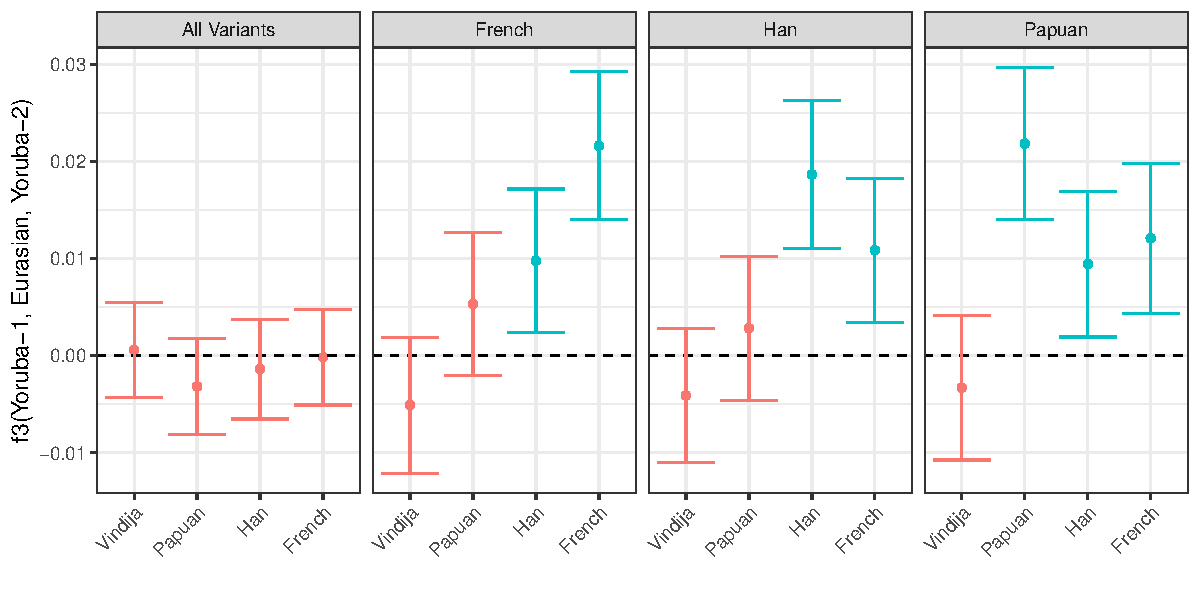
\includegraphics[width = \textwidth]{plot/f3.pdf}
  \slcaption{ $f_3$ statistics show evidence for shared drift with Eurasians. Following the reconstruction of putatively migrated segments from the inferred ancestral recombination graph, we use the Reich Human Origins data set to investigate admixture using drift statistics using {\tt ADMIXTOOLS} and {\tt admixr} (see URLs). Tests are separated into all markers, and those ascertained through {\tt SMCSMC} runs with the French, Han, and Papuans as a comparison Eurasian group. The $f_3$ statistics estimate is plotted, along with 95\% C.I. computed via a block jackknife. Statistics which are significantly larger than zero are coloured blue, indicating shared drift.}
  \label{fig:f3}
\end{figure}


\begin{figure}
  \centering
  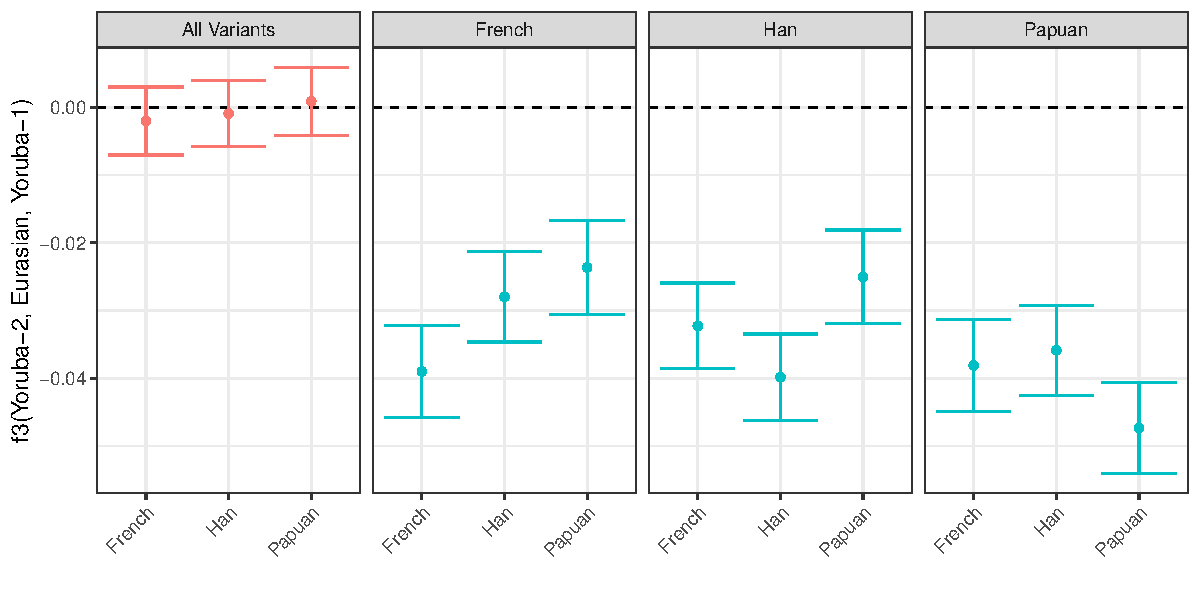
\includegraphics[width=\textwidth]{plot/f3_admix.pdf}
  \slcaption{$f_3$ statistics show evidence for Eurasian admixture. Following the reconstruction of putatively migrated segments from the inferred ancestral recombination graph, we use the Reich Human Origins data set to investigate admixture using drift statistics using {\tt ADMIXTOOLS} and {\tt admixr} (see URLs). Tests are separated into all markers, and those ascertained through {\tt SMCSMC} runs with the French, Han, and Papuans as a comparison Eurasian group. The $f_3$ statistics estimate is plotted, along with 95\% C.I. computed via a block jackknife. Statistics which are significantly less than zero indicate statistical evidence for admixture, and are coloured blue.}
  \label{fig:f3_admix}
\end{figure}

We use $D$ statistics to examine more nuanced scenarios. We find that the two Yorubans share more alleles than other groups in Africa (D(African group, Yoruba-1; Yoruba-2, Chimp) is significantly negative with $|Z|>3$), but the individual of interest is closer to Out of Africa (OoA) groups such as the Han, French, and Papauns (D(OoA, Yoruba-2; Yoruba-1, Chimp) is significantly negative with $|Z|<3$) than to its partner Yoruban (\Cref{dstats:a1}). This implies that SMCSMC has identified segments of the African Genome which are more closely related to OoA populations than to fellow Africans.   


In summary, we find no evidence for gene flow with a Vindija Neanderthal on the Mbuti baseline, or when compared to a different Yoruban (\Cref{dstats:a5}, \Cref{dstats:a4}). We additionally find no evidence for increased affinity to the Vindija Neanderthal when compared to the Altai, as would be expected if the material were descended from admixing Eurasians (\Cref{dstats:a6}). However, we find that restricted to the identified segments, $D$ statistics have power to detect evidence for the known admixture from Vindija into a French individual (\Cref{dstats}), suggesting that lack of power does not explain the lack of evidence we find for Neanderthal admixture into Africans.  In addition, we find no differences in affinity to Neanderthals or Denisovans between the variants which fall in segments and the whole genome (\Cref{dstats}d). Taken together, this suggests that Eurasian-derived segments of the African genomes are not enriched with Neanderthal material.


\begin{figure}
	\centering
	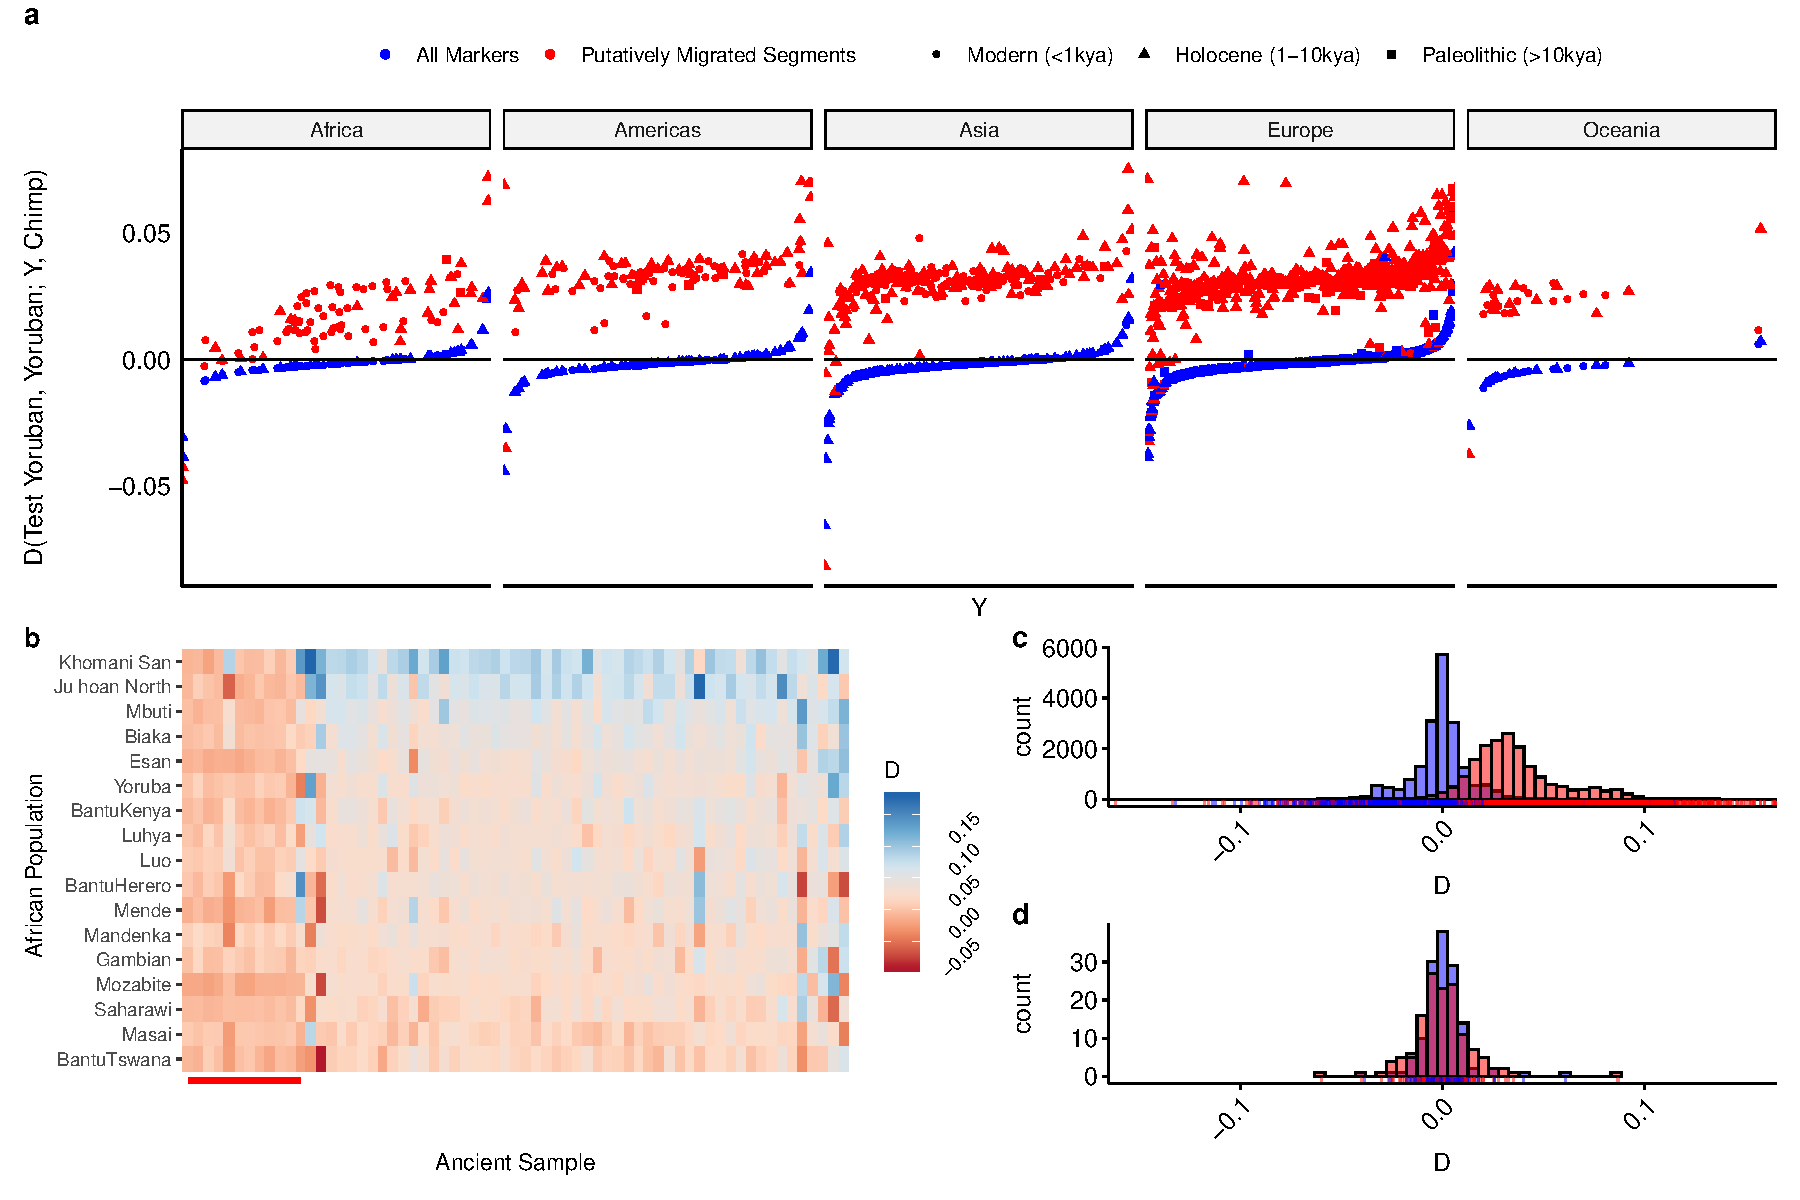
\includegraphics[width=\textwidth]{plot/new_dstats.pdf}
	\slcaption{African introgressed segments are more similar to Eurasians but show no Neanderthal or Denisovan enrichment. {\bf a.} $D$(Test Yoruban, Comparison Yoruban; Test population, Chimpanzee) calculated for all populations in the Reich Human Origins dataset (see URLs). $D$ statistics in the putatively migrated segments are higher across the board in 3589 ancient, 6472 present day individuals. {\bf b.} The same $D$ statistic but computed for all African populations and individuals sampled from the Paleolithic. Neanderthal and Denisovan samples (marked with red bar) show low affinity to a Yoruban in putatively migrated segments. {\bf c.} Histogram of $D$ statistics computed in a. showing clear inflation of statistics calculated in segments (red) versus all markers (blue). {\bf d.} Subset of individuals from a. involving Neanderthal ($n = 6$),  Denisovan ($n=1$), and a unique mixture individual ($n=1$) with statistics calculated in segments (red) and all markers (blue) for all $n=17$ African individuals indicating no difference in this population.} 
	\label{dstats}
\end{figure}



% latex table generated in R 3.6.2 by xtable 1.8-4 package
% Thu Jan 30 15:10:56 2020
\begin{table}[ht]
  \centering
  \begin{tabular}{lrr}
    \hline
  Statistic & D & Z \\ 
    \hline
  D(KhomaniSan-1, Yoruba-1, Yoruba-2, Chimp) & -0.181 & -28.403 \\ 
    D(Mbuti-1, Yoruba-1, Yoruba-2, Chimp) & -0.135 & -19.554 \\ 
    D(Papuan-1, Yoruba-1, Yoruba-2, Chimp) & -0.026 & -3.422 \\ 
    D(French-1, Yoruba-1, Yoruba-2, Chimp) & -0.006 & -0.866 \\ 
    D(Han-1, Yoruba-1, Yoruba-2, Chimp) & 0.001 & 0.072 \\ 
    D(KhomaniSan-1, Yoruba-2, Yoruba-1, Chimp) & -0.187 & -28.109 \\ 
    D(Mbuti-1, Yoruba-2, Yoruba-1, Chimp) & -0.130 & -19.323 \\ 
    D(Papuan-1, Yoruba-2, Yoruba-1, Chimp) & -0.008 & -1.003 \\ 
    D(French-1, Yoruba-2, Yoruba-1, Chimp) & 0.030 & 4.355 \\ 
    D(Han-1, Yoruba-2, Yoruba-1, Chimp) & 0.056 & 8.037 \\ 
     \hline
  \end{tabular}
  \slcaption{Putatively migrated segments of a Yoruban are closer to Out of Africa groups than a comparable Yoruban.} 
  \label{dstats:a1}
  \end{table}
  
  % latex table generated in R 3.6.2 by xtable 1.8-4 package
  % Thu Jan 30 15:10:56 2020
  \begin{table}[ht]
  \centering
  \begin{tabular}{lrr}
    \hline
  Statistic & D & Z \\ 
    \hline
  D(Mbuti-1, Yoruba-1, Vindija, Chimp) & -0.001 & -0.141 \\ 
    D(Mbuti-1, Yoruba-2, Vindija, Chimp) & -0.003 & -0.306 \\ 
     \hline
  \end{tabular}
  \slcaption{No difference in allele sharing with Vindija Neanderthal over Mbuti baseline.} 
  \label{dstats:a5}
  \end{table}
  
  % latex table generated in R 3.6.2 by xtable 1.8-4 package
  % Thu Jan 30 15:10:56 2020
  \begin{table}[ht]
  \centering
  \begin{tabular}{lrr}
    \hline
  Statistic & D & Z \\ 
    \hline
  D(Yoruba-2, Yoruba-1, Vindija, Chimp) & 0.000 & 0.012 \\ 
     \hline
  \end{tabular}
  \slcaption{No difference in allele sharing with Vindija Neanderthal.} 
  \label{dstats:a4}
  \end{table}
  
  % latex table generated in R 3.6.2 by xtable 1.8-4 package
  % Thu Jan 30 15:10:56 2020
\begin{table}[ht]
\centering
\begin{tabular}{lrr}
  \hline
Statistic & D & Z \\ 
  \hline
D(Vindija, Altai, Yoruba-1, Chimp) & 0.024 & 1.095 \\ 
  D(Vindija, Altai, Yoruba-2, Chimp) & 0.034 & 1.526 \\ 
  D(Vindija, Altai, Mbuti-1, Chimp) & 0.002 & 0.103 \\ 
  D(Vindija, Altai, KhomaniSan-1, Chimp) & 0.023 & 1.008 \\ 
    \hline
\end{tabular}
\slcaption{No increased affinity to Vindija Neanderthal over Altai, as would be expected if the source of any Neanderthal ancestry was Eurasian.} 
\label{dstats:a6}
\end{table}



\section{Discussion}
We have developed an approach for estimating demographic parameters and ARGs from whole genome sequence data, which can handle inference in complex demographic models, and implemented this in the software program SMCSMC \cite{Henderson2018}. We used SMCSMC to investigate ancient migration rates and population substructure, and found evidence for a substantial admixture from ancestors of present-day Eurasian populations into African populations in the Late Middle Paleolithic.

Our analysis suggests that a population ancestral to present-day Eurasians contributed as much as a third of the genetic material in many modern African populations. We find no difference in inferred admixture proportions when using French Europeans or Han Chinese as extant representatives of the donor population, indicating that the admixing population must have split from the out-of-Africa population before the East/West Eurasian divergence, implying a lower bound on the timing of the admixture of approximately 40kya \cite{Mathieson2014}. It appears that our results suggest that the migrating population was more similar to present-day French and Chinese populations than to Papuans.  However, up to 5\% of the genomes of some present-day Papuans have been suggested to derive from archaic introgressions \cite{Sankararaman2016}, and these contributions will have reduced the inferred levels of admixture into Africans when using Papuans as a representative of the Eurasian ancestors.
The alternative explanation, of an earlier divergence of Papuans and Eurasian ancestors, is possible but contested; in light of documented Eurasian admixture into Oceania, the effects of this early isolation are likely to be small relative to the large confounding effects of Denisovan admixture \cite{Malaspinas2016, Nielsen2017a}.

The proposed period of admixture has biased previous inferences of the African population sizes. We show that including directional migration into the model resolves previously unexplained high inferred $N_e$ in the period $80$ to $300$kya. It is well known that effective population size estimates are biased in the presence of population substructure and migration \cite{Chikhi2018, Li2011}. We use simulations to show that the proposed admixture event indeed causes an increase in estimated $N_e$ in analyses that do not explicitly model migration.  Correctly modeling of directional migration recovers the correct $N_e$, and allows us to infer a more recent split time between the two populations than indicated by previous analyses, although we did not attempt to formally estimate this time of divergence.

We found that not all populations in Africa have been equally affected by the proposed migration event. While the ancestors of Niger-Kordofanian and Nilo-Saharan populations show evidence of similar levels of Eurasian admixture, the ancestors of Central African and South African hunter-gatherer populations show markedly lower levels.  The date of genetic diversification of both the Central Hunter Gatherers and Khoe-San (SAHG) is contested \cite{Lipson2019}, but a date of $100$kya has been proposed \cite{Schlebusch2012}, providing a putative upper bound on the main admixture event.  Our simulations indicate that SMCSMC has little power to detect the impact of migration events occurring more than $70$kya, providing an additional upper bound on the time of the migration episode, or the fraction of it that left a sufficiently distinct imprint on extant genetic material.

Compared to the remainder of the Niger-Kordofanians and Nilo-Saharans on the one hand, and the SAHG populations on the other, the Mbuti and Biaka show intermediate levels of admixture. Of these populations, the Biaka show slightly higher levels of admixture than the Mbuti, which is likely due to the well-documented admixture from Western African groups not shared with the Mbuti \cite{Batini2011}. The lower levels of admixture in Mbuti and Biaka compared to Niger-Kordofian and Nilo-Saharan populations imply at least partial diversification of the former at the time of the migration, placing an upper bound on the timing. However, dating the diversification of these groups is difficult. Recent estimates using $f$ statistics place the split concurrent with the San in a large-scale early expansion 200-250kya \cite{Lipson2019}, while older data consistently report an earlier split time between 50 and 90 kya \cite{Patin2018}. Further clarity on the early structure and diversification of hunter-gatherer populations are necessary to interpret their interactions with Eurasian migrants. The  Afroasiatic populations on the other hand show high levels of admixture, which also appears to be of much more recent origin, and it appears likely that this is the result of extensive admixture from Eurasian populations during the Holocene \cite{Busby2016, Fan2019}. 

It has previously been suggested that Eurasian back-migration may be responsible for Neanderthal material in Africans \cite{Chen2020}; however, we find no evidence for enrichment of Neanderthal-like material in putatively Eurasian-derived genomic segments in Africans based on a sample from the posterior distribution of \glspl{arg}. We expect that this sample \gls{arg} is representative of the underlying demographic process across the whole genome; we find no evidence of shared drift between African populations and representative Neanderthal samples in isolated admixture segments across the entire genome. This observation indicates that Neanderthal introgression into Eurasians occurred after the African introgression event we study here, or that further population structure in the Eurasian ancestral population precluded substantial transmission of Neanderthal material into Africa.

Our findings are consistent with several other published observations. Migration rate estimates using {\tt MSMC-IM} revealed high levels of admixture at times comparable to our results \cite{Wang2019a}. The coalescent intensity function additionally shows similar histories between sub-Saharan African and Eurasian groups with high coalescent intensity in epochs consistent with our inference and those of {\tt MSMC-IM}, supporting both an early split between the groups and a substantial replacement of genetic material more recently than $\sim100$kya \cite{Albers2019}. Evidence has been mounting for multiple migrations into the Eurasian continent, possibly mediated by climatic drivers \cite{Timmermann2016, Pagani2016}. Eurasian backflow during the Holocene has been well established \cite{Lopez2015, GallegoLlorente2015}, but earlier migrations have also been proposed before based on observations of the spatial distribution of Y chromosome and mitochondrial haplogroups \cite{Altheide1997, Hammer1998, Cruciani2002, Chandrasekar2007, Cabrera2018, Hervella2016, Haber2019}. At the same time, evidence has been mounting for extreme heterogeneity in the history of sub-Saharan Africans, with several unsampled populations theorised to have contributed at various points in the past \cite{Lipson2019, Durvasula2019, Speidel2019}. In light of these recent studies, the observations in this paper add to a growing body of evidence for complex population structure and migration surrounding the Out of Africa event leading to a substantial replacement of the African population in the Late Middle Paleolithic.  

\section{Acknowledgments}

The SMCSMC project began in 2013, more than four years before I began my DPhil with Gerton Lunter. At that time, Sha (Joe) Zhu and Gerton Lunter developed the core of the analytical method and derived many of the mathematical innovations presented in the article (deriving waypoints, the extension of particle filters for continuous Markov jump processes). Donna Henderson devoted the majority of her DPhil to fine-tuning the method and performing many core aspects of quality control and validation. She mainly applied her work to an understanding of Neanderthal introgressions throughout history. My place in this project comes after Donna and Joe both completed their DPhils and postdoctoral fellowships respectively. I contributed substantially to the software implementation of the SMC2 project as well as validation of the method, as well as the work presented in this thesis describing its application to inferring directional migration rates.